\documentclass[envcountsame,envcountchap, openany, 14pt]{mysvmono2}
% \documentclass[14pt]{report}
\usepackage{blindtext}
\usepackage[paperheight=29.7cm,paperwidth=21.0cm, top=2.5cm, bottom=2cm, left=3.5cm, right=2cm]{geometry}
\usepackage[ddmmyyyy]{datetime}
%!TEX root = book_ML.tex
% \usepackage[margin=1in]{geometry}
\usepackage[T5]{fontenc}
% \setcounter{secnumdepth}{3}
\setcounter{tocdepth}{2} %% depth level of table of content with 0 - chapter only 
\usepackage[utf8]{inputenc}
\usepackage{amsmath}
\usepackage{amssymb}
% \usepackage{amssymb,amsbsy}
% \setlength{\parindent}{0em}
\setlength{\parskip}{1em}
% choose options for [] as required from the list
% in the Reference Guide, Sect. 2.2

% ******************************************************************************
%% force table caption to top 
%https://tex.stackexchange.com/questions/22751/how-to-force-table--on-top
\usepackage{floatrow}
\floatsetup[table]{capposition=top}
\usepackage[font={sf,  }, tableposition=top]{caption}
\usepackage{subcaption}
\DeclareCaptionFormat{rule}{#1#2#3\rule{\textwidth}{.0pt}}
% \DeclareCaptionFormat{norule}{}
\DeclareCaptionLabelFormat{mylabel}{#1 #2.\hspace{1.5ex}}
\captionsetup[figure]{labelformat=mylabel, labelfont = bf, justification=justified, labelsep=none}
%%% change name Table and Figure
\captionsetup[table]{name=Bảng}
\captionsetup[figure]{name=Hình}
% \captionsetup[listing]{name=Code}

% caption on side
\usepackage{floatrow}
\usepackage{sidecap}

% ******************************************************************************


\usepackage{graphicx}        % standard LaTeX graphics tool
                             % when including figure files
\usepackage{multicol}        % used for the two-column index
\usepackage[bottom]{footmisc}% places footnotes at page bottom
% etc.
% see the list of further useful packages
% in the Reference Guide, Sects. 2.3, 3.1-3.3
% rule after figure
% \usepackage{caption}
% \usepackage[tableposition=top]{caption}

\usepackage{xcolor}
\def\myrule{\textcolor{gray}{\rule{\textwidth}{.1pt}}}
% \def\myrulethin{\rule{\textwidth}{.01pt}}

\usepackage{multirow}
%%%%%%%%%%
\usepackage{makeidx}         % allows index generation
\makeindex             % used for the subject index
                       % please use the style svind.ist with
                       % your makeindex program


\usepackage{silence}
\WarningFilter{latex}{Composite letter}
\WarningFilter{latex}{Package hyperref Warning: Composite letter}


\usepackage{cite,url,bm}
% \usepackage{hyperref}
% \urlstyle{rm}
% \usepackage[unicode]{hyperref}
\usepackage[unicode, pdftex,
            pdfauthor={Pham Hong Thai},
            pdftitle={Phan tich thanh phan chinh}]{hyperref}
\renewcommand\UrlFont{\sffamily}
\hypersetup{
    colorlinks=black,
    linkcolor=black,
    filecolor=magenta,
    urlcolor=blue,
}

%%%%%%%%%%%%%%%%%%%5
% \usepackage{listings}
% \usepackage{color}
% \usepackage{textcomp}
% %New colors defined below
% \definecolor{codegreen}{rgb}{0,0.6,0}
% \definecolor{codegray}{rgb}{0.5,0.5,0.5}
% \definecolor{codepurple}{rgb}{0.58,0,0.82}
% \definecolor{backcolour}{rgb}{0.95,0.95,0.92}


% \makeatletter
% \expandafter\let\csname active@char\string?\endcsname\relax
% \expandafter\let\csname active@char\string!\endcsname\relax
% \expandafter\let\csname active@char\string:\endcsname\relax


% \initiate@active@char{?}
% \initiate@active@char{!}
% \initiate@active@char{:}
% \makeatletter



\usepackage{courier}

\usepackage{listings}
\renewcommand{\lstlistingname}{Code}
% \usepackage[T1]{fontenc}
\usepackage{xcolor}
\usepackage{textcomp}
%Code listing style named "mystyle"
% \lstdefinestyle{mystyle}{
%   backgroundcolor=\color{backcolour},   commentstyle=\color{codegreen},
%   keywordstyle=\color{magenta},
%   stringstyle=\color{codepurple},
%   basicstyle=\footnotesize,
%   frame = single,
%   breakatwhitespace=false,
%   breaklines=true,
%   captionpos=b,
%   keepspaces=true,
%   numbers=none,
%   numbersep=5pt,
%   showspaces=false,
%   showstringspaces=false,
%   showtabs=false,
%   tabsize=2,
%   basicstyle=\footnotesize\ttfamily,
%   % columns = flexible, 
%   keepspaces = true,
% }

\definecolor{codegreen}{rgb}{0,0.6,0}
\definecolor{codegray}{rgb}{0.5,0.5,0.5}
\definecolor{codepurple}{rgb}{0.58,0,0.82}

\definecolor{codegreen}{rgb}{1, 1, 1}
\definecolor{codegray}{rgb}{.2, .2, .2}
\definecolor{codepurple}{rgb}{0, 0, 0}
\definecolor{codekey}{rgb}{0, 0, 0}
\definecolor{backcolour}{rgb}{1, 1, 1}


\usepackage{courier}

\lstdefinestyle{mystyle}{
  backgroundcolor=\color{backcolour},  
  commentstyle=\color{codegray} \itshape,
  keywordstyle=\color{codekey} \bfseries,
  numberstyle=\tiny\color{codekey},
  stringstyle=\color{codepurple},
  basicstyle=\ttfamily\footnotesize\color{codekey},
  % basewidth  = {.5em,0.5em},
  % basicstyle=\ttfamily,
  breakatwhitespace=false,         
  breaklines=true,                 
  captionpos=b,                    
  keepspaces=true,                 
  numbers=none,                    
  numbersep=5pt,                  
  showspaces=false,                
  showstringspaces=false,
  showtabs=false,                  
  tabsize=4, 
  frame = single,
  framesep = 7pt,
  % columns = flexible, 
  % keepspaces = false
}

%"mystyle" code listing set
\lstset{style=mystyle}





\lstset{style=mystyle}
\lstset{basicstyle=\footnotesize\ttfamily,breaklines=true}


% Default fixed font does not support bold face
\DeclareFixedFont{\ttb}{T1}{txtt}{bx}{n}{11} % for bold
\DeclareFixedFont{\ttm}{T1}{txtt}{m}{n}{10}  % for newtcbtheoremal

% Custom colors
% \usepackage{color}
\definecolor{deepblue}{rgb}{0,0,0}
\definecolor{deepred}{rgb}{0,0,0}
\definecolor{deepgreen}{rgb}{0,0,0}


% % Python style for highlighting
\newcommand\pythonstyle{\lstset{
language=Python,
basicstyle=\ttm,
otherkeywords={self},             % Add keywords here
keywordstyle=\ttb\color{deepblue},
emph={MyClass,__init__},          % Custom highlighting
emphstyle=\ttb\color{deepred},    % Custom highlighting style
stringstyle=\color{deepgreen},
frame=tb,                         % Any extra options here
showstringspaces=false            %
}}


\usepackage{colortbl}

% \include{myenv}
\usepackage{tcolorbox}
\usepackage{wrapfig}
\newtcolorbox{mybox}[3][]
{
  colframe = #2!25,
  colback  = #2!10,
  coltitle = blue,  
  title    = \textbf{#3},
  #1,
}



%% ========= long bar notation ==============================
\makeatletter
\newsavebox\myboxA
\newsavebox\myboxB
\newlength\mylenA
\newcommand*\lbar[2][.75]{%
    \sbox{\myboxA}{$\m@th#2$}%
    \setbox\myboxB\null% Phantom box
    \ht\myboxB=\ht\myboxA%
    \dp\myboxB=\dp\myboxA%
    \wd\myboxB=#1\wd\myboxA% Scale phantom
    \sbox\myboxB{$\m@th\overline{\copy\myboxB}$}%  Overlined phantom
    \setlength\mylenA{\the\wd\myboxA}%   calc width diff
    \addtolength\mylenA{-\the\wd\myboxB}%
    \ifdim\wd\myboxB<\wd\myboxA%
       \rlap{\hskip 0.5\mylenA\usebox\myboxB}{\usebox\myboxA}%
    \else
        \hskip -0.3\mylenA\rlap{\usebox\myboxA}{\hskip 0.3\mylenA\usebox\myboxB}%
    \fi}
\makeatother

%%%%%%%%%%%% wide hat 
\def\what{\widehat}



% ******************************************************************************
% custom environments
\tcbuselibrary{theorems}
\tcbuselibrary{skins,raster}
\newtcbtheorem[number within=chapter]{mytheo}{Định lý}{colback=white,colframe=gray,fonttitle=\bfseries}{th}

\newtcbtheorem[number within=chapter]{mydef}{Định nghĩa}{colback=white,colframe=gray,fonttitle=\bfseries}{def}

\newtcbtheorem[number within=chapter]{myalg}{Thuật toán}{colback=white,colframe=gray,fonttitle=\bfseries, fontupper = \itshape}{alg}

% \newenvironment{myalg}
    % {
    % \begin{tcolorbox}[colback = blue!5, colframe=gray, title = Thuật toán,fonttitle=\bfseries]
    % \it
    % }
    % {
    % \end{tcolorbox}
    % }

\newenvironment{mydeff}
    {
    \begin{tcolorbox}[colback=white,colframe=gray, title = Chú ý,fonttitle=\bfseries]
    \it
    }
    {
    \end{tcolorbox}
    }
 
\newenvironment{mynote}
    {
    \begin{tcolorbox}[colback = white!5, colframe=gray, title =,fonttitle=\bfseries]
    \it
    }
    {
    \end{tcolorbox}
    }

\newcommand{\newnote}[2]{
    % 1: title, 2: content 
    \begin{tcolorbox}[colback = white, leftrule = .3mm, rightrule = .3mm, toprule = .3mm, bottomrule = .3mm, colframe=black, title =#1,fonttitle=\bfseries]
    \it
    #2    
    \end{tcolorbox}
}

\newcommand{\myeqnbox}[1]{
    % 1: content 
    \begin{tcolorbox}[toptitle = 0mm, leftrule = .3mm, rightrule = .3mm, toprule = .3mm, bottomrule = .3mm, colback = white, colframe=black, sharp corners]    
    \abovedisplayskip=-10pt
    \belowdisplayskip=-30pt
    #1
    \end{tcolorbox}
}


\newenvironment{myfr}
    {\begin{center} \it
    \begin{tcolorbox}[colback = yellow!20, colframe=yellow!45!black]
    % \includegraphics[width = 2cm]{logo.png}
    \begin{wrapfigure}{L}{0.1\textwidth}
    \vspace{-100pt}
    \href{https://google.com}{
    \includegraphics[width=\textwidth]{pgfs/logofundaml.pdf}}
    \vspace{-30pt}
    \end{wrapfigure}
    }
    {
    \end{tcolorbox}
    \end{center}
    }
% END custom environments
% ******************************************************************************

% ******************************************************************************
% definitions 
\def\etal{\textit{et al.}}

\def\ba{\mathbf{a}}
\def\bb{\mathbf{b}}
\def\bd{\mathbf{d}}
\def\be{\mathbf{e}}
\def\bm{\mathbf{m}}
\def\bK{\mathbf{K}}
\def\bk{\mathbf{k}}
\def\bM{\mathbf{M}}
\def\bp{\mathbf{p}}
\def\bq{\mathbf{q}}
\def\bx{\mathbf{x}}
\def\by{\mathbf{y}}
\def\bz{\mathbf{z}}
\def\bu{\mathbf{u}}
\def\bv{\mathbf{v}}
\def\bw{\mathbf{w}}

\def\bbx{\bar{\mathbf{x}}}
\def\bbX{\bar{\mathbf{X}}}
\def\bbw{\bar{\mathbf{w}}}

\def\bE{\mathbf{E}}
\def\bX{\mathbf{X}}
\def\bY{\mathbf{Y}}
\def\bZ{\mathbf{Z}}
\def\bA{\mathbf{A}}
\def\bB{\mathbf{B}}
\def\bC{\mathbf{C}}
\def\bP{\mathbf{P}}
\def\bQ{\mathbf{Q}}
\def\bI{\mathbf{W}}
\def\bS{\mathbf{S}}
\def\bT{\mathbf{T}}
\def\bW{\mathbf{W}}
\def\bI{\mathbf{I}}
\def\bL{\mathbf{L}}
\def\bU{\mathbf{U}}
\def\bzero{\mathbf{0}}
\def\bone{\mathbf{1}}
\def\R{\mathbb{R}}
\def\L{\mathcal{L}} 
\def\S{\mathcal{S}} 


\def\bmt{\left[\begin{matrix}}
\def\bmt{\end{matrix}\right]}

\def\diag{\text{diag}}

\def\bmt{\left[\begin{matrix}}
\def\emt{\end{matrix}\right]}

\def\blambda{\boldsymbol{\lambda}}
\def\bxi{\boldsymbol{\xi}}
\def\bSigma{\mathbf{\Sigma}}
\def\bLambda{\boldsymbol{\Lambda}}
\def\bnu{\boldsymbol{\nu}}
\def\bmu{\boldsymbol{\mu}}

% \def\dpcm{\hfill $\square$} % Điều phải chứng minh. 
\def\dpcm{} % Điều phải chứng minh. 
\def\tcr{\textcolor{red}}
\def\tcb{\textcolor{blue}}
\def\trace{\text{trace}}
\def\rank{\text{rank}}
\def\sgn{\text{sgn}}
\def\assign{\leftarrow}
\def\imply{\Rightarrow}
\def\dom{\textbf{dom}}

\def\lg{\textit{\textbf{Lời giải}}:}
\def\vd{\textbf{Ví dụ}: }
\def\kq{{{Kết quả:}}}
% ******************************************************************************

% ******************************************************************************
% Python environment
\lstnewenvironment{python}[1][]
{
\pythonstyle
\lstset{#1}
}
{}
% Python for external files
\newcommand\pythonexternal[2][]{{
\pythonstyle
\lstinputlisting[#1]{#2}}}
% Python for inline
\newcommand\pythoninline[1]{{\color{deepred}\pythonstyle\lstinline!#1!}}

\newcommand{\bi}[1]{\textit{\textbf{{#1}}}} % bold and italic 
% ******************************************************************************

% ******************************************************************************
%%%%%%%%% Header and {Footer}
\usepackage{fancyhdr}
\pagestyle{fancy}
\fancyhf{}
\fancyhead[LE,RO]{\nouppercase\leftmark}
% \fancyhead[RE,LO]{\thepage}
% \fancyfoot[RE,LO]{}
% \fancyfoot[LE,RO]{Trang \thepage}

\rfoot{Trang \thepage}

\fancypagestyle{plain}{%
\fancyhf{}
\renewcommand{\headrulewidth}{0pt}
}



\renewcommand{\headrulewidth}{.2pt}
\renewcommand{\footrulewidth}{.1pt}
% ******************************************************************************

\DeclareMathOperator*{\argmin}{argmin}
\DeclareMathOperator*{\argmax}{argmax}



%%%%%% definition

% ******************************************************************************
%%%%%% chapter
\makeatletter
\def\thickhrulefill{\leavevmode \leaders \hrule height 1.2ex \hfill \kern \z@}
\def\@makechapterhead#1{
  \vspace*{10\p@}%
  {\parindent \z@ \centering \reset@font
        \thickhrulefill\quad
        \scshape\bfseries\textit{\@chapapp{}  \thechapter}
        % \scshape\bfseries{\Large CHƯƠNG  \thechapter}
        \quad \thickhrulefill
        \par\nobreak
        \vspace*{10\p@}%
        \interlinepenalty\@M
        \hrule
        \vspace*{10\p@}%
        \Huge \bfseries #1 \par\nobreak
        \par
        \vspace*{10\p@}%
        \hrule
        \vskip 100\p@
  }}
% ******************************************************************************



% ******************************************************************************
% title 
\title{
% {\centering \bf Machine Learning cơ bản}\\
\\

\\
% {\small First Edition}
% Lần cập nhật gần nhất:
\vspace{-1.2cm}
}




\usepackage[compact]{titlesec}
\titlespacing{\section}{0pt}{*0}{*0}
\titlespacing{\subsection}{0pt}{*0}{*0}
\titlespacing{\subsubsection}{0pt}{*0}{*0}
% ******************************************************************************

%% for book cover 
\usepackage{incgraph,tikz}
\usetikzlibrary{patterns}
\newlength{\hatchspread}
\newlength{\hatchthickness}
\newlength{\hatchshift}
\newcommand{\hatchcolor}{}
% declaring the keys in tikz
\tikzset{hatchspread/.code={\setlength{\hatchspread}{#1}},
         hatchthickness/.code={\setlength{\hatchthickness}{#1}},
         hatchshift/.code={\setlength{\hatchshift}{#1}},% must be >= 0
         hatchcolor/.code={\renewcommand{\hatchcolor}{#1}}}
% setting the default values
\tikzset{hatchspread=6pt,
         hatchthickness=0.15pt,
         hatchshift=0pt,% must be >= 0
         hatchcolor=black}
% declaring the pattern
\pgfdeclarepatternformonly[\hatchspread,\hatchthickness,\hatchshift,\hatchcolor]% variables
   {custom north west lines}% name
   {\pgfqpoint{\dimexpr-2\hatchthickness}{\dimexpr-2\hatchthickness}}% lower left corner
   {\pgfqpoint{\dimexpr\hatchspread+2\hatchthickness}{\dimexpr\hatchspread+2\hatchthickness}}% upper right corner
   {\pgfqpoint{\dimexpr\hatchspread}{\dimexpr\hatchspread}}% tile size
   {% shape description
    \pgfsetlinewidth{\hatchthickness}
    \pgfpathmoveto{\pgfqpoint{0pt}{\dimexpr\hatchspread+\hatchshift}}
    \pgfpathlineto{\pgfqpoint{\dimexpr\hatchspread+0.15pt+\hatchshift}{-0.15pt}}
    \ifdim \hatchshift > 0pt
      \pgfpathmoveto{\pgfqpoint{0pt}{\hatchshift}}
      \pgfpathlineto{\pgfqpoint{\dimexpr0.15pt+\hatchshift}{-0.15pt}}
    \fi
    \pgfsetstrokecolor{\hatchcolor}
%    \pgfsetdash{{1pt}{1pt}}{0pt}% dashing cannot work correctly in all situation this way
    \pgfusepath{stroke}
   }


\tikzstyle{shaded}=[pattern = custom north west lines]

% ******************************************************************************
% section number too close to headers in table of content
% Source: https://tex.stackexchange.com/questions/219160/toc-spacing-between-number-and-header
%
% \usepackage{titletoc}

% \titlecontents{chapter}[0em]{\vspace{.25\baselineskip}}
% {\eqparbox{ch}{\bfseries\thecontentslabel}\enspace}{}
% {\hspace{.5em}\hfill\contentspage}

% \titlecontents{section}[1.8em]{\vspace{.25\baselineskip}}
% {{\thecontentslabel}\enspace}{}
% {\hspace{.5em}\titlerule*[10pt]{$\cdot$}\contentspage}

% \titlecontents{subsection}[4.5em]{\vspace{.25\baselineskip}}
% {\eqparbox{Ss}{\thecontentslabel}\enspace}{}
% {\hspace{.5em}\titlerule*[10pt]{$\cdot$}\contentspage}

% \newcommand*\l@section{\@dottedtocline{1}{1.5em}{2.3em}}
% \newcommand*\l@subsection{\@dottedtocline{2}{3.8em}{3.2em}}
% \newcommand*\l@subsubsection{\@dottedtocline{3}{7.0em}{4.1em}}
% \newcommand*\l@paragraph{\@dottedtocline{4}{10em}{5em}}
% \newcommand*\l@subparagraph{\@dottedtocline{5}{12em}{6em}}

% ******************************************************************************

%%%%%%%%%%%%%
%% Blank page 
%%%%%%%%%%%
\usepackage{afterpage}

\newcommand\blankpage{%
    \null
    \thispagestyle{empty}%
    \addtocounter{page}{-1}%
    \newpage}


%%%%%%%%%%%%%%%%%%%%%%%%%%%%%%%%%%%%%%%%%%%%%%%%%5
% boxed around eqnarray
% source: https://tex.stackexchange.com/questions/109900/how-can-i-box-multiple-aligned-equations

% \newcommand*\widefbox[1]{\fbox{\hspace{2em}#1\hspace{2em}}}

% \usepackage{amsmath}
% \usepackage{empheq}
% \usepackage[theorems,skins]{tcolorbox}

% \newtcolorbox{mymathbox}[1][]{colback=white, sharp corners, #1}

% \usepackage{amsmath}
% add (.) into section number. E.g: 1.1., 1.2., 
\usepackage{titlesec}
\titlelabel{\thetitle.~}
% continous footnote numbering.
\usepackage{chngcntr}
\counterwithout{footnote}{chapter}

\usepackage{enumitem}
% \usepackage{enumerate}
\def\myenum{label=\alph*)}
\setenumerate[0]{label=\alph*.}      

%%%%%% format subsubsection to bold italic
\usepackage{titlesec}
\titleformat*{\subsubsection}{\bfseries\itshape}


\usepackage{natbib}
% \setlength{\bibsep}{5.0pt}
\usepackage{indentfirst}
\usepackage{makecell}
% \usepackage{pbox}
\begin{document}
\frontmatter%%%%%%%%%%%%%%%%%%%%%%%%%%%%%%%%%%%%%%%%%%%%%%%%%%%%%%
\mainmatter%%%%%%%%%%%%%%%%%%%%%%%%%%%%%%%%%%%%%%%%%%%%%%%%%%%%%%%

% %% cover
% \incgraph[documentpaper, overlay={\node[red] at (page.center) {};}][width=\paperwidth]{Chapters/cover/cover1.png}

\section*{\centering Lời cảm ơn}

Lời đầu tiên, em xin bày tỏ sự cảm ơn chân thành đối với Cô giáo, TS.
Nguyễn Thị Mỹ Bình – giáo viên hướng dẫn trực tiếp em.

Em cũng xin gửi lời cảm ơn tới các thầy cô trong khoa Công nghệ thông tin,
trường Đại học Công Nghiệp Hà Nội đã hướng dẫn, chỉ bảo và tạo điều kiện cho em
học tập cũng như nghiên cứu trong thời gian qua.

Cảm ơn Câu lạc bộ HIT, Đội Olympic Tin học khoa Công nghệ thông tin đã đồng hành
cùng em trong suốt quãng thời gian học tập, làm việc tại trường.

Mặc dù đã cố gắng hoàn thành báo cáo đồ án tốt nghiệp này nhưng chắc chắn
sẽ không tránh khỏi những sai sót, em kính mong nhận được sự thông cảm và chỉ
bảo của các thầy cô và các bạn.

\tableofcontents

%!TEX root = ../book_ML.tex
% \addtocontents{toc}{\protect\newpage}
\chapter{Lời nói đầu}
\label{part:dimred}


\index{giảm chiều dữ liệu -- dimensionality reduction}
\index{dimensionality reduction -- giảm chiều dữ liệu}
\index{lựa chọn đặc trưng -- feature selection}
\index{feature selection -- lựa chọn đặc trưng}
\index{trích chọn đặc trưng -- feature extraction}
\index{feature extraction -- trích chọn đặc trưng}

\chapter*{MỞ ĐẦU}
\markboth{Mở đầu}{}
\addcontentsline{toc}{chapter}{MỞ ĐẦU}
\label{part:dimred}

\section{Lý do chọn đề tài}

Với sự phát triển không ngừng của khoa học và công nghệ, đặc biệt là với những
chiếc điện thoại thông minh (smartphone) ngày càng hiện đại và được sử dụng
phổ biến trong đời sống con người đã làm cho lượng thông tin thu được bằng hình ảnh
ngày càng tăng. Theo đó, lĩnh vực xử lý ảnh cũng được chú trọng phát triển, ứng dụng
rộng rãi trong đời sống xã hội hiện đại. Không chỉ dừng lại ở việc chỉnh sửa, tăng
chất lượng hình ảnh mà với công nghệ xử lý ảnh hiện nay chúng ta có thể giải quyết
các bài toán nhận dạng chữ viết, nhận dạng dấu vân tay, nhận dạng khuôn mặt...
Một trong những bài toán được nhiều người quan tâm nhất của lĩnh vực xử lý ảnh hiện nay
đó là nhận dạng khuôn mặt (Face Recognition). Như chúng ta đã biết, khuôn mặt đóng
vai trò quan trọng trong quá trình giao tiếp giữa người với người, nó mang một lượng
thông tin giàu có, chẳng hạn như từ khuôn mặt chúng ta có thể xác định giới tính, tuổi tác,
chủng tộc, trạng thái cảm xúc, đặc biệt là xác định mối quan hệ với đối tượng (có quen biết
hay không).


Do đó,bài toán nhận dạng khuôn mặt đóng vai trò quan trọng trong nhiều lĩnh vực
đời sống hằng ngày của con người như các hệ thống giám sát, quản lý vào
ra, tìm kiếm thông tin một người nổi tiếng,...đặc biệt là an ninh, bảo mật.
Có rất nhiều phương pháp nhận dạng khuôn mặt để nâng cao hiệu suất tuy nhiên dù ít hay
nhiều những phương pháp này đang vấp phải những thử thách về độ sáng, hướng nghiêng,
kích thước ảnh, hay ảnh hưởng của tham số môi trường. Bài toán
Nhận diện khuôn mặt (Face Recognition) bao gồm nhiều bài toán khác nhau như:
phát hiện mặt người (face detection), đánh dấu (facial landmarking), trích chọn(rút) đặc trưng
(feature extration), gán nhãn, phân lớp (classification).
Trong thực tế, nhận dạng khuôn mặt người (Face Recognition) là một hướng nghiên cứu được
nhiều nhà khoa học quan tâm, nghiên cứu để ứng dụng trong thực tiễn.
Vì thế có những cải tiến nghiên cứu về bài toán phát hiện khuôn mặt người trong
những môi trường phức tạp hơn, có nhiều khuôn mặt người trong ảnh hơn,
và có nhiều tư thế thay đổi trong ảnh... Trong bài này tôi sẽ tìm hiểu về trích rút đặc
trưng sử dụng học sâu (Deep learning) và áp dụng vào bài toán nhận diện khuôn mặt .

% Chúng ta sẽ xem xét các phương pháp giảm chiều dữ liệu phổ biến
% nhất: \textit{phân tích thành phần chính} ({principle component analysis}) cho bài toán giảm chiều dữ liệu
% vẫn giữ tối đa lượng thông tin, và \textit{linear discriminant analysis}
% cho bài toán giữ lại những đặc trưng quan trọng nhất cho việc phân loại. Trước
% hết, chúng ta cùng tìm hiểu một phương pháp phân tích ma trận vô
% cùng quan trọng  --  \textit{phân tích giá trị suy biến} ({singular value decomposition}).

\section{Mục đích của đề tài}

\begin{itemize}
    \item Xây dựng, tìm kiếm các mô hình học sâu để trích xuất thông tin khuôn mặt
          người dùng 1 cách chính xác, hiệu quả.
    \item Tìm hiểu sử dụng thành thạo các phương pháp làm giàu dữ liệu,
          ứng dụng cho bài toán nhận diện với dữ liệu là các ảnh khuôn mặt
    \item Xây dựng các phương pháp thu thập dữ liệu
    \item Tìm hiểu ứng dụng các thuật toán phân loại trong học máy để
          áp dụng vào bài toàn nhận diện khuôn mặt
\end{itemize}

\section{Đối tượng và phạm vi nghiên cứu của đề tài}
\subsection{Đối tượng}
\begin{itemize}
    \item Các mô hình học sâu nổi tiếng về nhận dạng khuôn mặt được các nhà khoa học huấn luyện trước với nhưng bộ dữ liệu
          cực lớn và chuẩn xác.
    \item Các mô hình, phương pháp phát hiện khuôn mặt trong ảnh với độ chính xác cao
    \item Các phương pháp làm giàu dữ liệu, đặc biệt là với dữ liệu khuôn mặt.
    \item Các phương pháp phân loại dữ liệu trong học máy và học sâu
    \item Các phương pháp đánh giá mất mát thương dùng để huấn luyện các mô hình học máy, học sâu
\end{itemize}

\subsection{Phạm vi nghiên cứu}
\begin{itemize}
    \item Tập trung sử dụng bộ dữ liệu tự tạo của các sinh viên trong trường đại học Công nghiệp Hà Nội
    \item Huấn luyện mô hình theo phương pháp đánh giá bộ ba (triplet loss)
    \item Sử dụng các đánh giá cơ bản để đánh giá tính chính xác của mô hình
\end{itemize}

\newpage
\section{Kết cấu của đồ án}
Gồm 4 chương:

Chương 1 : Nghiên cứu tổng quan

Chương 2 : Cơ sở lý thuyết

Chương 3 : Thiết kế và xây dựng hệ thống

Chương 4 : Kết luận và hướng phát triển


\section{Lời cảm ơn}

Lời đầu tiên, em xin bày tỏ sự cảm ơn chân thành đối với Cô giáo, ThS.
Nguyễn Thị Mỹ Bình – giáo viên hướng dẫn trực tiếp em.

Em cũng xin gửi lời cảm ơn tới các thầy cô trong khoa Công nghệ thông tin,
trường Đại học Công Nghiệp Hà Nội đã hướng dẫn, chỉ bảo và tạo điều kiện cho em
học tập cũng như nghiên cứu trong thời gian qua.

Cảm ơn Câu lạc bộ HIT, Đội Olympic Tin học khoa Công nghệ thông tin đã đồng hành
cùng em trong suốt quãng thời gian học tập, làm việc tại trường.

Mặc dù đã cố gắng hoàn thành Báo cáo thực tập tốt nghiệp nhưng chắc chắn
sẽ không tránh khỏi những sai sót, em kính mong nhận được sự thông cảm và chỉ
bảo của các thầy cô và các bạn.

%!TEX root = ../book_ML.tex

\def\R{\mathbb{R}}
\newpage
\section{Bảng các ký hiệu}
Các ký hiệu sử dụng trong sách được liệt kê trong Bảng~\ref{tab:notation}.

\begin{table}[h]
    \caption{Các quy ước ký hiệu và tên gọi được sử dụng trong báo cáo}
    \label{tab:notation}
    \centering
    \begin{tabular}{|c|l|}
    \hline 
    Ký hiệu & Ý nghĩa  \\ \hline 
    \hline 
    $x, y, N, k$ & in nghiêng, thường hoặc hoa, là các số vô hướng \\ \hline
    $\bx, \by$ & in đậm, chữ thường, là các vector  \\ \hline
    $\bX, \bY$ & in đậm, chữ hoa, là các ma trận  \\ \hline
    $\R$ & tập hợp các số thực \\ \hline 
    $\mathbb{N}$ & tập hợp các số tự nhiên \\ \hline 
    $\mathbb{C}$ & tập hợp các số phức \\ \hline 
    $\R^{m}$ & tập hợp các vector thực có $m$ phần tử \\ \hline 
    $\R^{m\times n}$ &tập hợp các ma trận thực có $m$ hàng, $n$ cột \\ \hline
    $\mathbb{S}^n$ & tập hợp các ma trận vuông đối xứng bậc $n$ \\ \hline 
    $\mathbb{S}^n_{+}$ & tập hợp các ma trận nửa xác định dương bậc $n$ \\
    \hline 
    $\mathbb{S}^n_{++}$ & tập hợp các ma trận xác định dương bậc $n$ \\ \hline 
    $ \in $ & phần tử thuộc tập hợp \\ \hline 
    $ \exists $ & tồn tại \\ \hline 
    $ \forall $ & mọi \\ \hline 
    $ \triangleq$ & ký hiệu là/bởi. Ví dụ $a\triangleq f(x)$ nghĩa là ``ký hiệu
    $f(x)$ bởi $a$''. \\ \hline 
    $x_i$ & phần tử thứ $i$ (tính từ 1) của vector $\bx$ \\ \hline 
    $\sgn(x)$ & hàm xác định dấu. Bằng 1 nếu $x \geq 0$, bằng -1 nếu $x < 0$. \\ \hline
    $\exp(x)$ & $e^x$ \\ \hline
    $\log(x)$ & logarit \textit{tự nhiên} của số thực dương $x$ \\ \hline
    $\displaystyle \argmin_xf(x)$ & giá trị của $x$ để hàm $f(x)$ đạt giá trị nhỏ nhất \\ \hline 
    $\displaystyle \argmax_xf(x)$ & giá trị của $x$ để hàm $f(x)$ đạt giá trị lớn nhất \\ \hline 
    % $a_{ij}$ & phần tử hàng thứ $i$, cột thứ $j$ của ma trận $\bA$ \\ \hline 
    % $\bA^T$ & chuyển vị của ma trận $\bA$ \\ \hline 
    % $\bA^H$ & chuyển vị liên hợp (Hermitian) của ma trận phức $\bA$ \\ \hline 
    % $\bA^{-1}$ & nghịch đảo của ma trận vuông $\bA$, nếu tồn tại \\ \hline 
    % $\bA^{\dagger}$ & giả nghịch đảo của ma trận không nhất thiết vuông $\bA$ \\
    % \hline 
    % $\bA^{-T}$ & chuyển vị của nghịch đảo của ma trận $\bA$, nếu tồn tại \\ \hline 
    % $\|\bx\|_p$ & $\ell_p$ norm của vector $\bx$ \\ \hline  
    % $\|\bA\|_F$ &  Frobenius norm của ma trận $\bA$ \\ \hline 
    % $ \diag(\bA)$ & đường chéo chính của ma trận $\bA$ \\ \hline 
    % $\trace(\bA)$ & trace của ma trận $\bA$ \\ \hline 
    % $\det(\bA)$ & định thức của ma trận vuông $\bA$ \\ \hline 
    % $\text{rank}(\bA)$ & hạng của ma trận $\bA$ \\ \hline 
    o.w & \textit{otherwise}  --  trong các trường hợp còn lại \\ \hline 
    $\displaystyle\frac{\partial f}{\partial x}$ & đạo hàm của hàm số $f$ theo $x \in \R$ \\ \hline
    $\nabla_{\bx}f$ & gradient của hàm số $f$ theo $\bx$ ($\bx$ là vector hoặc ma trận) \\ \hline 
    $\nabla^2_{\bx}f$ & gradient bậc hai của hàm số $f$ theo $\bx$, còn được gọi là \textit{Hesse} \\ \hline 
    $\odot$ & \makecell{Hadamard product (elemenwise product). Phép nhân từng phần tử \\ của hai vector hoặc ma trận cùng kích thước.} \\ \hline 
    $\propto$ & tỉ lệ với \\ \hline 
    % v.v. & vân vân \\ \hline 
    %%%%%%%
    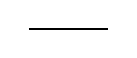
\begin{tikzpicture}
    \draw [thick] (0, 0) -- (1, 0); 
    \end{tikzpicture}
    & đường nét liền \\ \hline 

    %%%%%%%
    \begin{tikzpicture}
    \draw [very thick, dashed] (0, 0) -- (1, 0); 
    \end{tikzpicture}
    & đường nét đứt \\ \hline 

    %%%%%%%
    \begin{tikzpicture}
    \draw [very thick, dotted] (0, 0) -- (1, 0); 
    \end{tikzpicture}
    & đường nét chấm (đường chấm chấm)\\ \hline 

    %%%%%%%
    \begin{tikzpicture}
    \draw [very thick, dash pattern={on 7pt off 2pt on 1pt off 3pt}] (0,0) -- (1,0);
    \end{tikzpicture}
    & đường chấm gạch\\ \hline 
    %%%%%%%
    % \\[-3mm]
    % \vspace{1em}
    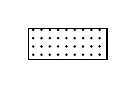
\begin{tikzpicture}[yshift = -1cm]
    \draw [pattern = dots] (0,0) rectangle (1,.4);
    \end{tikzpicture}
    & nền chấm\\\hline 
    %%%%%%%
    % \\[-1em]
    % \vspace{1em}
    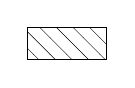
\begin{tikzpicture}
    \draw [pattern = custom north west lines] (0,0) rectangle (1,.4);
    \end{tikzpicture}
    & nền sọc chéo\\ \hline 



    \end{tabular}
 \end{table} 

%!TEX root = ../../book_ML.tex
\chapter{Nghiên cứu tổng quan}
\label{cha: chap1}
% \index{principal component analysis}
% \index{PCA -- \textit{xem} principle component analysis}
% \index{PCA}

% \index{phân tích thành phần chính -- principle component analysis}
% \index{principle component analysis -- phân tích thành phần chính}
% \index{PCA}
\section{Các phương pháp nghiên cứu}

\begin{itemize}
    \item Hiện nay có 2 phương pháp nhận diện khuôn mặt được sử dụng rộng rãi nhất là:
          \begin{itemize}
              \item Nhận dạng dựa trên các đặc trưng của các phần tử trên khuôn mặt
                    (Feature base face recognition)
              \item Nhận dạng dựa trên xét tổng thể khuôn mặt (Appearance based face
                    recognition)
          \end{itemize}

    \item Ngoài ra còn một số phương pháp về loại sử dụng mô hình về khuôn mặt:
          \begin{itemize}
              \item Nhận dạng 2D: Elastics Bunch Graph, Active Appearance Model.
              \item Nhận dạng 3D: 3D Morphale Model
          \end{itemize}
\end{itemize}

\section{Ưu nhược điểm của các phương pháp}
\subsection{Nhận dạng dựa trên các đặc trưng của các phần tử trên khuôn mặt: }

Đây là phương pháp nhận dạng khuôn mặt dựa trên viện xác định các đặc trưng hình
học của các chi tiết trên một khuôn mặt (vị trí, diện tích, hình dạng của mắt,
mũi, miệng, ...) và mối quan hệ giữa chúng (khoảng cách của hai mắt, khoảng cách
của hai lông mày, ...).

Ưu điểm của phương pháp này là nó gần với cách mà con người sử dụng để nhận biết
khuôn mặt. Hơn nữa với việc xác định đặc tính cà mối quan hệ, phương pháp này có
thể cho kết quả tốt trong các trường hợp ảnh có nhiều nhiễu như bị nghiêng, bị
xoay hoặc ánh sáng thay đổi.

Nhược điểm của phương pháp này là cài đặt thuật toán phức tạp do việc xác định
mối quan hệ giữa các đặc tính sẽ khó phân biệt. Mặt khác, với các ảnh kích thước
bé thì các đặc tính sẽ khó phân biệt.


\subsection{Nhận dạng dựa trên xét tổng thể khuôn mặt:}

Đây là phương pháp xem mỗi ảnh có kích thước RxC là một vector trong không gian
RxC chiều. Ta sẽ xây dựng một không gian mới có chiều nhỏ hơn sao chi khi biểu diễn
trong không gian có các đặc điểm chính của một khuôn mặt không bị mất đi.
Trong không gian đó, các ảnh cùng một người sẽ được tập trung lại một nhóm
gần nhau và cách xa các nhóm khác.

Ưu điểm của phương pháp này là tìm được các đặc tính tiêu biểu của đối tượng cần nhận
dạng mà không cần phải xác định các thành phần và mối quan hệ giữa các thành phần đó.
Phương pháp sử dụng thuật toán có thể thực hiện tốt với các ảnh có độ phân giải cao,
thu gọn ảnh thành một ảnh có kích thước nhỏ hơn. Có thể kết hợp các phương pháp khác
như mạng Nơ-ron, Support Vector Machine.

Nhược điểm của phương pháp này phân loại theo chiều phân bố lớn nhất của vector.
Tuy nhiên, chiều phân bố lớn nhất không phải lúc nào cũng mang lại hiệu qua
tốt nhất cho bài toán nhận dạng và đặc biệt là phương pháp này rất nhạy với nhiễu.

\subsection{Kết luận}

Vì kết quả nghiên cứu cuối cùng là ứng dụng với yêu cầu về độ chính xác cao, 
khả năng thích ứng linh hoạt, hoạt động ổn định trong môi trường thực tế và 
hoạt động với các camera với độ phân giải thấp. Tôi quyết định chọn phương pháp 
nhận dạng dựạ trên xét tổng thể khuôn mặt (Appearance based face recognition).


%!TEX root = ../../book_ML.tex
\chapter{Cơ sở lý thuyết}
\label{cha: chap2}
% \index{principal component analysis}
% \index{PCA -- \textit{xem} principle component analysis}
% \index{PCA}

% \index{phân tích thành phần chính -- principle component analysis}
% \index{principle component analysis -- phân tích thành phần chính}
% \index{PCA}
\section{Tổng quan về nhận diện khuôn mặt}

Nhận diện khuôn mặt (Face recogintion) đang được ứng dụng trong nhiều lĩnh vực.
Hệ thống nhận dạng khuôn mặt là một ứng dụng cho phép máy tính tự động xác định
hoặc nhận dạng một người nào đó từ một bức hình ảnh kỹ thuật số hoặc một khung
hình.

Nhận diện khuôn mặt là một bài toán phức tạp, đòi hỏi cần phải xử lý một
loạt các vấn đề.

Mỗi khuôn mặt đều có nhưng điểm mốc, những phần lồi lõm, hình dáng của các
bộ phận trên khuôn mặt như mắt, mũi, miệng,... Các hệ thống nhận diện định
nghĩa những điểm này là những điểm nút, và mỗi khuôn mặt có khoảng 80 nút như thế.

Ngày nay các mô hình học sâu đã phát triển một cách vượt trội, việc trích rút các đặc trưng của một
khuôn mặt ngày một đơn giản và trở lên vô cùng chính xác. Mặc dù chúng ta không thể biết các đặc trưng đấy
là những đặc trưng gì bởi cơ chế tự động học của các mô hình học sâu rất phức tạp. Nhưng chúng ta vẫn có thể
kiểm tra độ chính xác bằng cách đưa những đặc trưng này vào các mô hình phân loại, xác nhận, ... sau đó
tính toán độ chính xác trên những dữ liệu có được.


\section{Tìm hiểu về OpenCV và ngôn ngữ lập trình Python}

OpenCV (Open Source Computer Vision Library) là một thư viện các chức năng lập
trình chủ yếu nhắm vào tầm nhìn máy tính thời gian thực. OpenCV hỗ trợ nhiều ngôn
ngữ lập trình như C++, Python, Java,… và có sẵn trên các nền tảng khác nhau bao
gồm Windows, Linux, Mac OS, Android và iOS. Các giao diện cho các hoạt động
GPU tốc độ cao dựa trên CUDA và OpenCL cũng đang được phát triển tích cực.

Cấu trúc tổng quan của OpenCV bao gồm 5 phần chính. 4 trong 5 phần đó được chỉ ra
trong hình vẽ dưới.

\begin{figure}
    \begin{subfigure}{0.7\textwidth}
        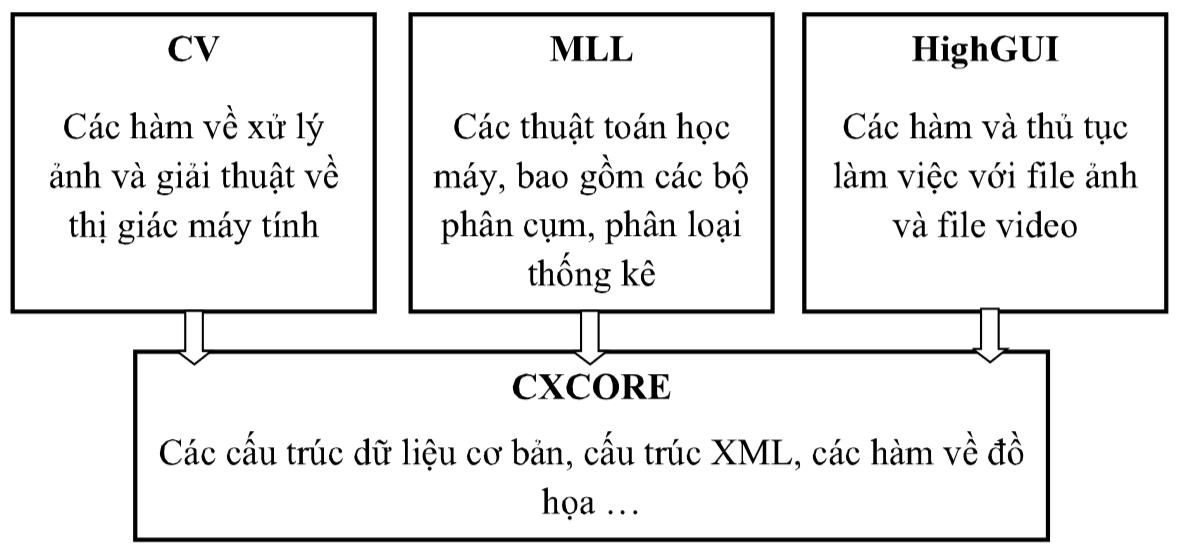
\includegraphics[width=0.99\linewidth]{Chapters/items/chap2_1.jpg}
        \caption{}
        \label{fig: chap2_1}
    \end{subfigure}
    \caption{Cấu trúc các phần của OpenCV.}
\end{figure}

Phần CV bao gồm các thư viện cơ bản về xử lý ảnh và các giải thuật về xử lý ảnh.
MLL là bộ thư viện về các thuật toán học máy, bao gồm rất nhiều bộ phân cụm và phân
loại thống kê. HighGUI chứa đựng những thủ tục vào ra, các chức năng về lưu trữ cũng
như đọc các file ảnh và video. Phần thứ 4, Cxcore chứa đựng các cấu trúc dữ liệu
cơ bản (ví dụ như cấu trúc XML, các cây dữ liệu …). Phần cuối cùng là CvAux, phần này
bao gồm các thư viện cho việc phát hiện, theo dõi và nhận dạng đối tượng (khuôn mặt, mắt …).

OpenCV - Python là một thư viện các ràng buộc Python được thiết kế để giải quyết các vấn đề
về xử lý ảnh và thị giác máy tính.

Python là ngôn ngữ lập trình có mục đích chung được bắt đầu bởi Guido van Rossum,
nó trở nên rất phổ biến rất nhanh trong thời gian gần đây, chủ yếu vì tính đơn giản
và khả năng đọc mã của nó. Nó cho phép lập trình viên thể hiện ý tưởng trong ít dòng
mã hơn mà không làm giảm khả năng đọc.

So với các ngôn ngữ như C/C++, Python chậm hơn. Điều đó nói rằng, Python có thể dễ dàng
được mở rộng với C/C++, cho phép chúng ta viết mã chuyên sâu tính toán trong C/C++
và tạo các trình bao bọc Python có thể được sử dụng làm mô-đun Python.
Điều này mang lại cho chúng ta hai lợi thế: thứ nhất, mã nhanh như mã C/C++ gốc
(vì đây là mã C++ thực tế hoạt động ở chế độ nền) và thứ hai, mã dễ dàng hơn trong
Python so với C/C++. OpenCV - Python là một trình bao bọc Python để thực hiện OpenCV C++
ban đầu.

OpenCV - Python sử dụng Numpy, một thư viện được tối ưu hóa cao cho các hoạt động số với
cú pháp kiểu MATLAB. Tất cả các cấu trúc mảng OpenCV được chuyển đổi sang và từ các mảng
Numpy. Điều này cũng giúp tích hợp dễ dàng hơn với các thư viện khác sử dụng Numpy
như SciPy và Matplotlib.



\section{Mô hình mạng neural tích chập (CNN - Convolutional neural network)}

Mạng neural tích chập (CNN) là một trong những mô hình học sâu\cite{repec} tiên tiến phổ biến nhất và
có ảnh hưởng nhất với cộng đồng thị giác máy tính (Computer vision). CNN thường được dùng
trong các bài toán nhận dạng ảnh, phân tích ảnh, xử lý ngôn ngữ tự nhiên dưới dạng ảnh các bước sóng.
Và hầu hết đều cho hiệu quả tốt đến rất tốt.

CNN là một kiến trúc mạng neural sinh ra để xử lý các dữ liệu phi cấu trúc dạng ảnh. Có 2 loại lớp
chính trong CNN: lớp tích chập (Convolutional layer) và lớp gộp (Pooling layer)

\begin{figure}
    \begin{subfigure}{1.\textwidth}
        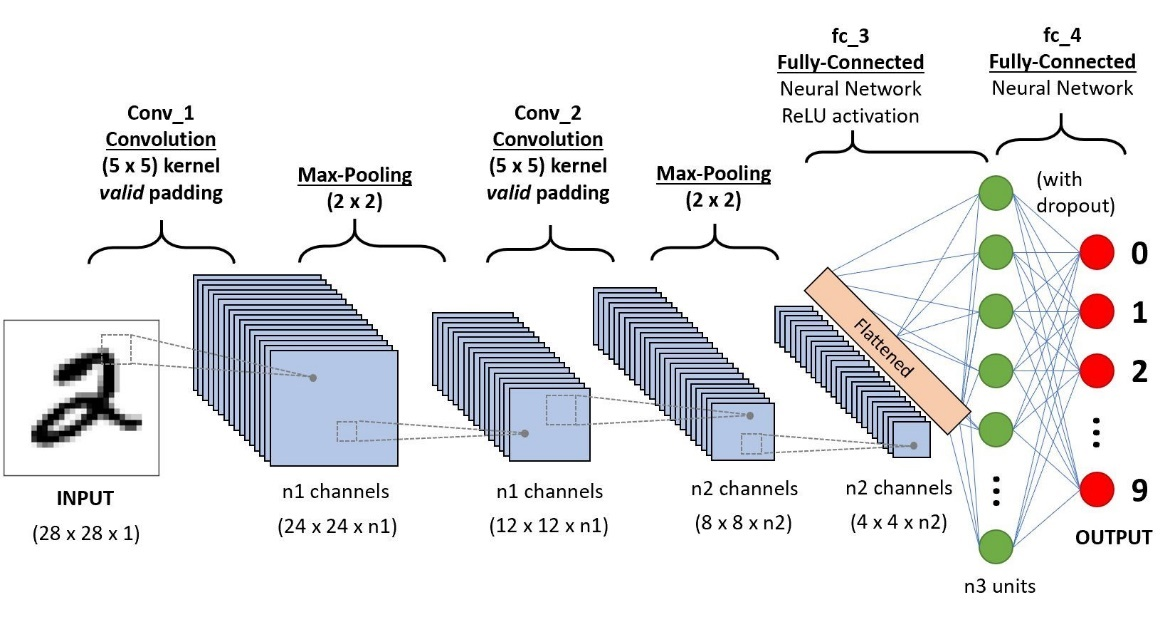
\includegraphics[width=1.\linewidth]{Chapters/items/cnn2_1.jpg}
        \label{fig: chap2_2}
    \end{subfigure}
    \caption{CNN cho bài toán nhận diện chữ số.}
\end{figure}
\subsection{Lớp tích chập}

Lớp tích chập là lớp quan trọng nhất và thường cũng là lớp đầu tiên của của mô hình CNN.
Lớp này có chức năng chính là phát hiện các đặc trưng có tính không gian hiệu quả.
Trong tầng này có 4 đối tượng chính là: ma trận đầu vào, bộ lọc (filters) và trường thụ cảm,
bản đồ đặc trưng (feature map). Lớp tích chập nhận đầu vào là một ma trận 3 chiều và một bộ lọc cần phải học.
Bộ lọc này sẽ trượt qua từng vị trí trên bức ảnh để tính tích chập (convolution)
giữa bộ lọc và phần tương ứng trên bức ảnh. Phần tương ứng này trên bức ảnh gọi là
trường thục cảm (receptive field), tức là vùng mà một neuron có thể nhìn thấy để đưa
ra quyết định, và mà trận cho ra bởi quá trình này được gọi là bản đồ đặc trưng (feature map).

Để hình dung, có thể tưởng tượng, bộ filters giống như các tháp canh trong nhà tù quét
lần lượt qua không gian xung quanh để tìm kiếm tên tù nhân bỏ trốn.
Khi phát hiện tên tù nhân bỏ trốn, thì chuông báo động sẽ reo lên, giống như các bộ lọc
tìm kiếm được đặc trưng nhất định thì tích chập đó sẽ cho giá trị tương ứng.

\begin{enumerate}
    \item Lớp tích chập được coi như xác định đặc trưng
          \begin{itemize}
              \item Lớp tích chập có chức năng chính là phát hiện đặc trưng cụ thể của bức ảnh.
                    Những đặc trưng này bao gồm đặc trưng cơ bản là góc, cạnh, màu sắc, hoặc đặc trưng
                    phức tạp hơn như texture của ảnh. Vì bộ lọc quét qua toàn bộ bức ảnh, nên những
                    đặc trưng này có thể nằm ở vị trí bất kì trong bức ảnh, cho dù ảnh bị xoáy trái/phải
                    thì những đặc trưng này vẫn bị phát hiện.
              \item Ở minh họa dưới, có một bộ lọc 5x5 dùng để phát hiện góc/cạnh, với bộ lọc này
                    chỉ có giá trị một tại các điểm tương ứng một góc cong.
                    \begin{figure}
                        \begin{subfigure}{0.6\textwidth}
                            \begin{center}
                                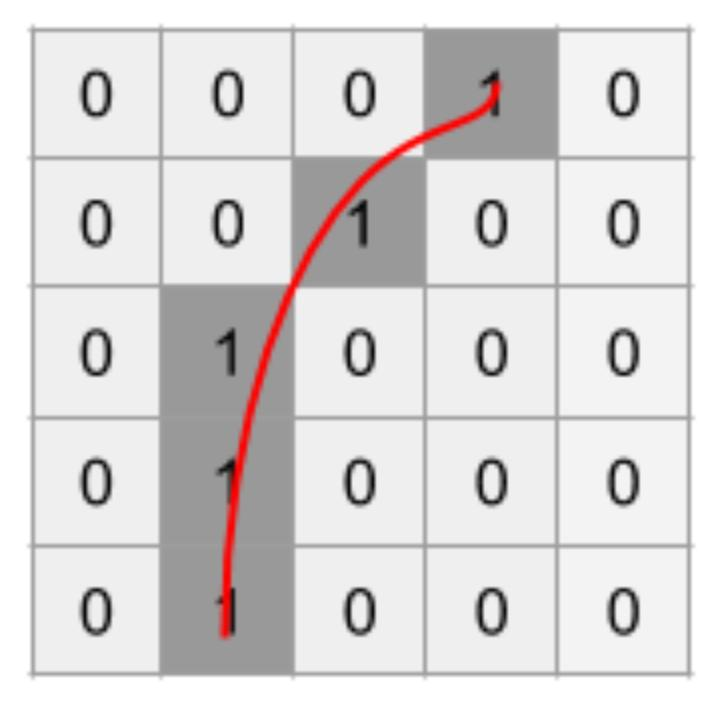
\includegraphics[width=0.6\linewidth]{Chapters/items/chap2_3.jpg}
                            \end{center}
                            \label{fig: chap2_3}
                        \end{subfigure}
                        \caption{Bộ lọc phát hiện cạnh}
                    \end{figure}
              \item Dùng bộ lọc ở trên trược qua ảnh của nhân vật Olaf trong trong bộ phim Frozen.
                    Chúng ta thấy rằng, chỉ ở những vị trí trên bức ảnh có dạng góc như đặc trưng ở
                    bộ lọc thì mới có giá trị lớn trên bản đồ đặc trưng, những vị trí còn lại sẽ cho giá trị
                    thấp hơn. Điều này có nghĩa là, bộ lọc đã phát hiện thành công một dạng góc/cạnh
                    trên dự liệu đầu vào. Tập hơn nhiều bộ lọc sẽ cho phép các bạn phát hiện được
                    nhiều loại đặc trưng khác nhau,và giúp định danh được đối tượng.
                    \begin{figure}
                        \begin{subfigure}{1.\textwidth}
                            \begin{center}
                                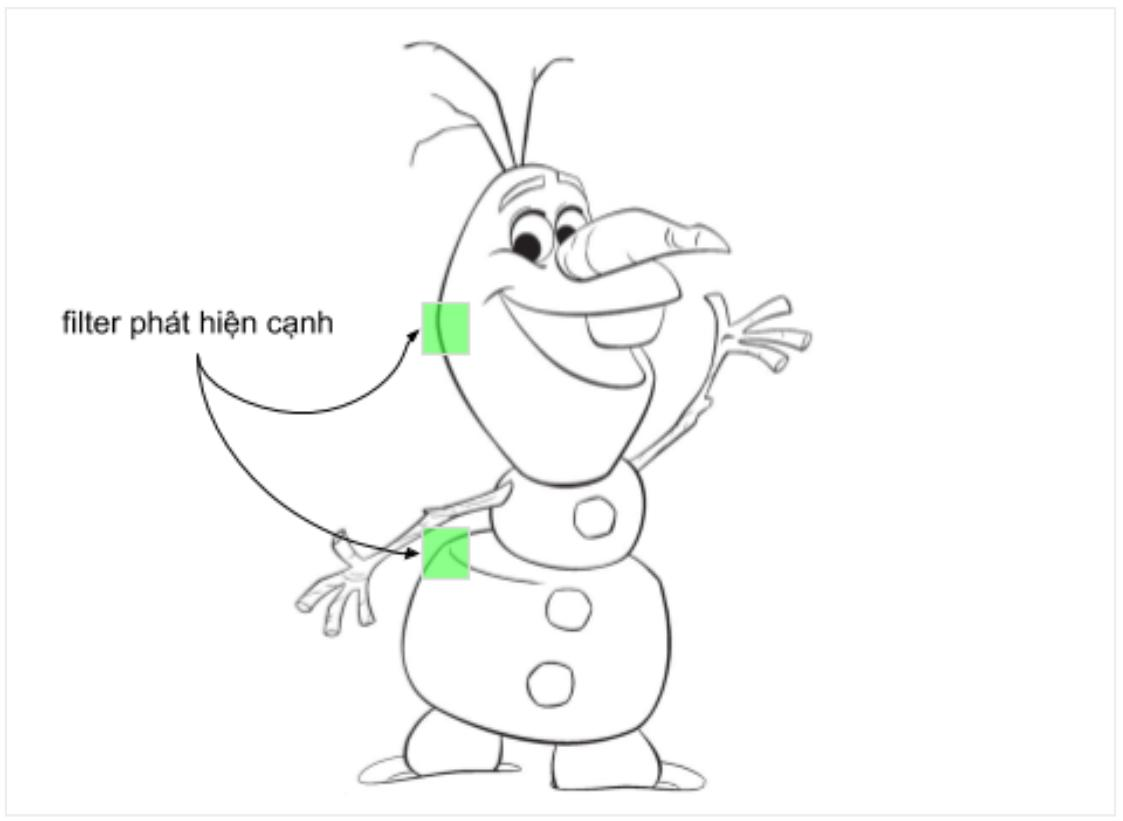
\includegraphics[width=1.\linewidth]{Chapters/items/chap2_4.jpg}
                            \end{center}
                            \label{fig: chap2_4}
                        \end{subfigure}
                        \caption{Bộ lọc phát hiện cạnh}
                    \end{figure}
          \end{itemize}
    \item Các tham số: Kích thước bộ lọc, bước nhảy, lề
          \begin{itemize}
              \item Kích thước bộ lọc là một trong những tham số quan trọng nhất của lớp tích chập.
                    Kích thước này tỉ lệ thuận với số tham số cần học tại mỗi lớp tích chập và
                    là tham số quyết định trường thụ cảm của tầng này. Kích thước phổ biến nhất của bộ lọc
                    là 3x3.
                    \begin{figure}
                        \begin{subfigure}{1.\textwidth}
                            \begin{center}
                                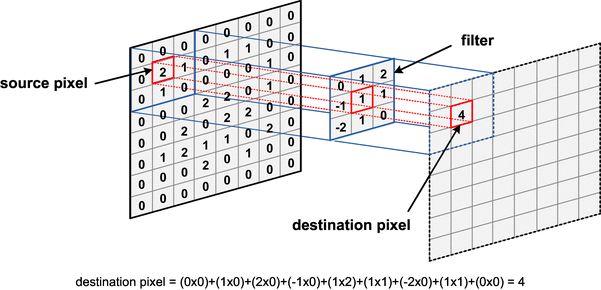
\includegraphics[width=1.\linewidth]{Chapters/items/chap2_5.jpg}
                            \end{center}
                            \label{fig: chap2_5}
                        \end{subfigure}
                        \caption{Cách hoạt động của bộ lọc (filter)}
                    \end{figure}
              \item Kích thước bộ lọc nhỏ được ưu tiên lựa chọn thay kích thước lớn vì những lý do sau đây:
                    \begin{itemize}
                        \item Cho phép nhìn được các vùng nhỏ
                        \item Trích rút được những đặc trưng có tính cục bộ cao
                        \item Phát hiện đặc trưng nhỏ
                        \item Đặc trưng được trích rút sẽ nhiều, đa dạng
                        \item Giảm kích thước ảnh chậm, cho phép mạng sâu hơn
                        \item Chia sẻ trọng số tốt hơn
                    \end{itemize}
              \item Kích thước của bộ lọc sẽ là những số lẻ để kết quả của phép tích chập sẽ nằm ở giữa ma trận
          \end{itemize}
\end{enumerate}

\subsection{Lớp phi tuyến}

Để các mô hình học sâu tìm được mối quan hệ phức tạp giữa các đặc trưng, cũng như tìm được những đặc trưng quan trọng
(là sự kết hợp phi tuyến giữa các đặc trưng cơ bản khác) thì các mối quan hệ đó khó có thể được biểu diễn dưới các hàm tuyến tính
mà cần sự kết hợp phi tuyến tính, chính vì vậy các hàm kích hoạt phi tuyến ra đời nhằm phá vỡ sự tuyến tính của giữa các đặc trưng từ đó tìm
ra các đặc trưng mới quan trọng hơn.

Hiện nay hàm kích hoạt được sử dụng phổ biến nhất là hàm ReLU (Rectified Linear Units). Hàm ReLU được ưa chuộm vì tính đơn giản và cho kết quả tốt hơn
ReLU cũng như những hàm kích hoạt khác, được đặt ngay sau tầng convolution, ReLU sẽ gán những giá trị âm bằng 0 và giữ nguyên giá trị của đầu vào khi lớn hơn 0.

ReLU cũng có một số vấn đề tiềm ẩn như không có đạo hàm tại điểm 0, giá trị của hàm ReLU có thể lớn đến vô cùng và
nếu chúng ta không khởi tạo trọng số cẩn thận, hoặc khởi tạo tỉ lệ học (learning rate) quá lớn thì những neuron ở tầng này sẽ rơi vào trạng thái chết, tức là luôn có giá trị < 0.

\begin{figure}
    \begin{subfigure}{1.\textwidth}
        \begin{center}
            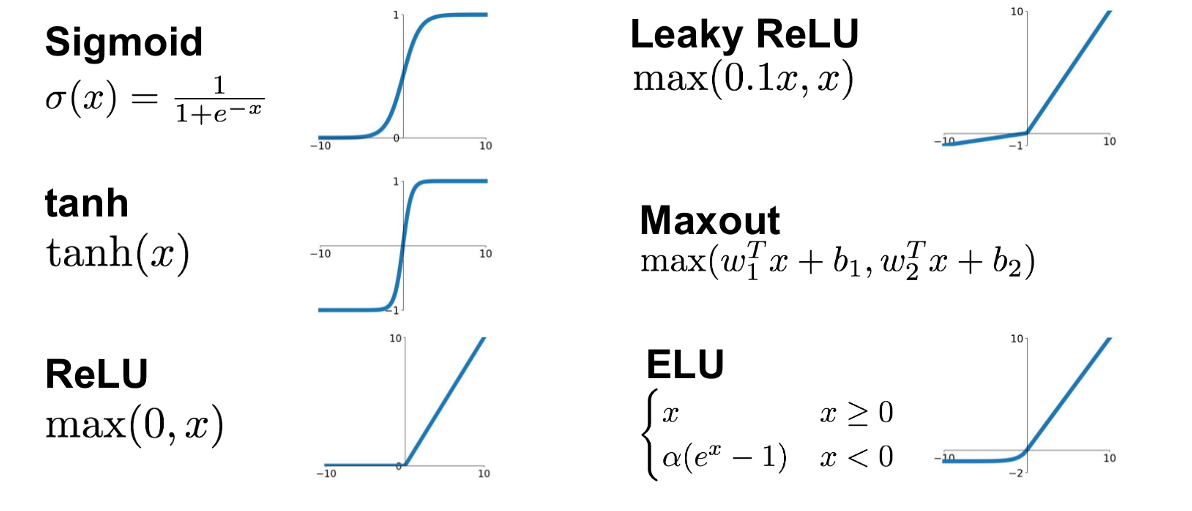
\includegraphics[width=1.\linewidth]{Chapters/items/chap2_6.jpg}
        \end{center}
        \label{fig: chap2_6}
    \end{subfigure}
    \caption{Một số hàm kích hoạt thường được sử dụng}
\end{figure}

\newpage
\subsection{Lớp gộp}

Sau hàm kích hoạt, thông thường chúng ta sử dụng lớp gộp. Một số loại lớp gộp phổ biến như là max-pooling, average pooling,
với chức năng chính là giảm chiều của tầng trước đó. Với một lớp gộp có kích thước 2x2,
các bạn cần phải trượt bộ lọc 2x2 này trên những vùng ảnh có kích thước tương tự rồi sau đó tính giá trị lớn nhất,
hay trung bình cho vùng ảnh đó.

\begin{figure}
    \begin{subfigure}{1.\textwidth}
        \begin{center}
            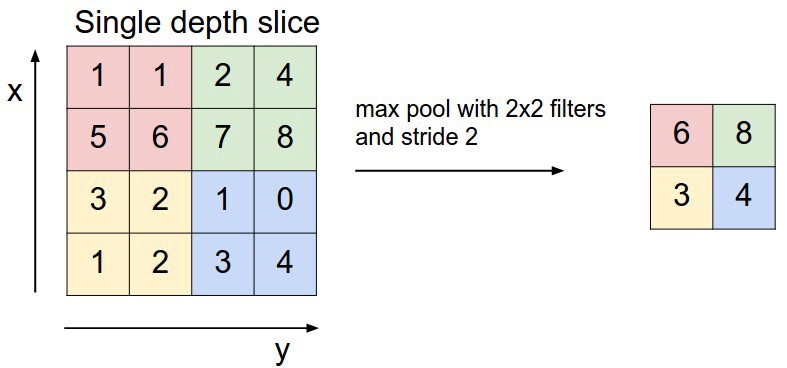
\includegraphics[width=1.\linewidth]{Chapters/items/chap2_7.jpg}
        \end{center}
        \label{fig: chap2_7}
    \end{subfigure}
    \caption{Ví dụ về max-pooling}
\end{figure}

Ý tưởng đằng sau lớp gộp là vị trí tuyết đối của những đặc trưng trong không gian ảnh không
còn cần cần thiết, thay vào đó vị trí tương đối giữ các đặc trưng đã đủ để phân loại đối tượng.
Hơn giảm tầng pooling có khả năng giảm chiều cực kì nhiều, làm hạn chế overfit,
và giảm thời gian huấn luyện tốt.

\newpage
\subsection{Lớp kết nối đầy đủ}

Lớp cuối cùng của mô hình CNN trong bài toán phân loại ảnh là lớp kết nối đầy đủ.
Lớp này có chức năng chuyển ma trận đặc trưng ở tầng trước thành các vector chứa xác suất của các
đối tượng cần được dự đoán.

Quá trình huấn luyện mô hình CNN cho bài toán phân loại ảnh cũng tương tự như huấn luyện các
mô hình khác. Cần có hàm đánh giá mất mát để tính sai số giữa dự đoán của mô hình và nhãn chính xác,
để sử dụng cơ chế của thuật toán lan truyền ngược (backprobagation) cho quá trình cập nhật trọng số.

\begin{figure}
    \begin{subfigure}{1.\textwidth}
        \begin{center}
            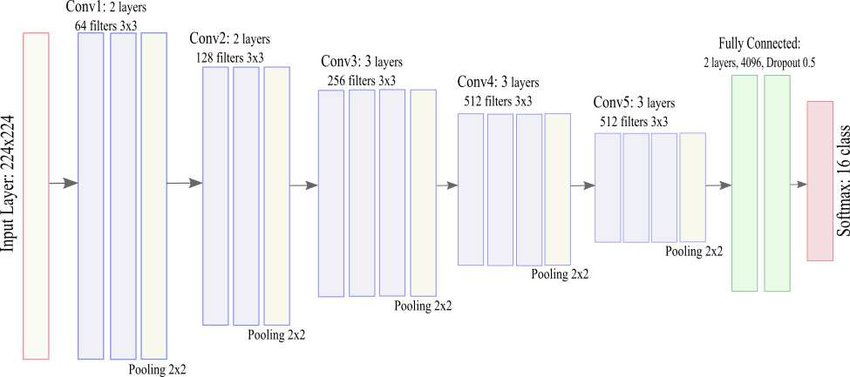
\includegraphics[width=1.\linewidth]{Chapters/items/chap2_8.jpg}
        \end{center}
        \label{fig: chap2_8}
    \end{subfigure}
    \caption{Một CNN đơn giản với đầy đủ các lớp}
\end{figure}

\newpage
\section{Máy dò khuôn mặt (Face detector)}

Để xác định các khuôn mặt\cite{detectface} trong các ảnh chứa nhiều yếu tố ngoại cảnh, và trích xuất các khuôn mặt đưa vào các
mô hình học sâu tiến hành trích xuất các đặc trưng của các khuôn mặt này thì phải dùng các máy dò khuôn mặt.

Hiện này có rất nhiều các máy dò khuôn mặt\cite{detectface1} được thiết kế bằng các mô hình học sâu khác nhau, ngay cả những máy dò được
thiết kế bằng các thuật toán xử lý ảnh thông thường cũng đã được phát triển và đạt hiệu quả tốt.
Ví dụ như các máy dò được tích hợp trong OpenCV (máy dò 5 điểm, 9 điểm, 68 điểm trên khuôn mặt). Nhưng để đạt được hiệu quả
tốt nhất có thể thì tôi sử dụng 1 máy dò có tên MTCNN (Multi-task Cascaded Convolutional Networks) được sử dụng phố biến
trong các hệ thống đòi hỏi sự chính xác cao.

\begin{figure}
    \begin{subfigure}{1.\textwidth}
        \begin{center}
            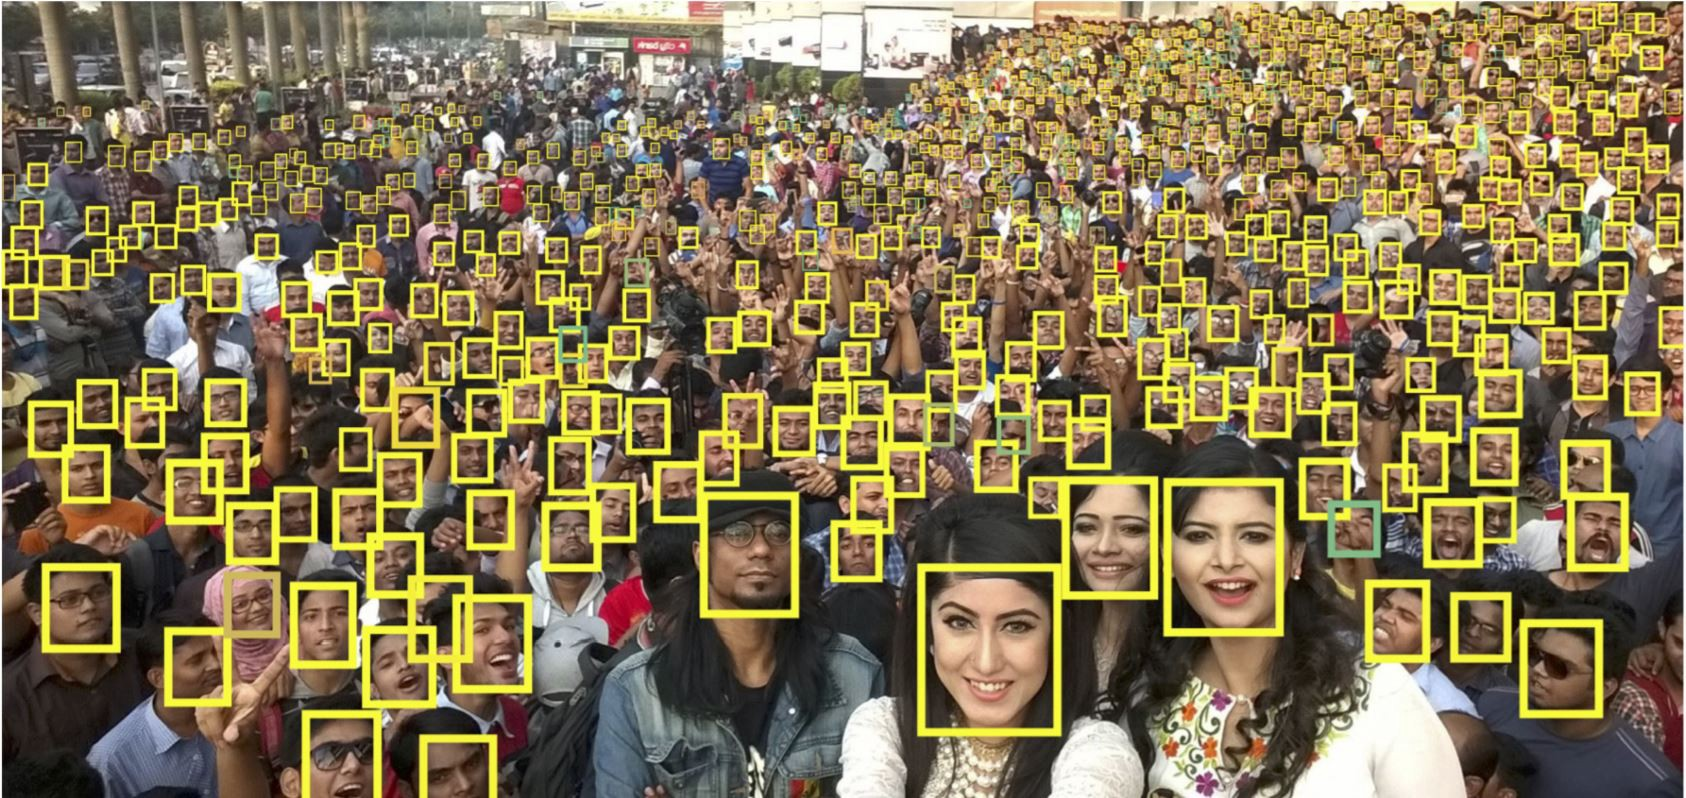
\includegraphics[width=1.\linewidth]{Chapters/items/chap2_test.jpg}
        \end{center}
        \label{fig: chap2_test}
    \end{subfigure}
    \caption{Ví dụ máy dò khuôn mặt}
\end{figure}

\newpage
\subsection{MTCNN}

MTCNN\cite{mtcnn} là viết tắt của Multi-task Cascaded Convolutional Networks (Mạng đa năng xếp tầng đa tác vụ).
Nó là bao gồm 3 mạng CNN xếp chồng và đồng thời hoạt động khi detect khuôn mặt.
Mỗi mạng có cấu trúc khác nhau và đảm nhiệm vai trò khác nhau trong task.
Đầu ra của MTCNN là vị trí khuôn mặt và 5 điểm trên mặt: mắt, mũi, miệng…

MTCNN hoạt động theo 3 bước, mỗi bước có một mạng neural riêng lần lượt là: P-Net, R-Net và O-net

\begin{figure}
    \begin{subfigure}{1.\textwidth}
        \begin{center}
            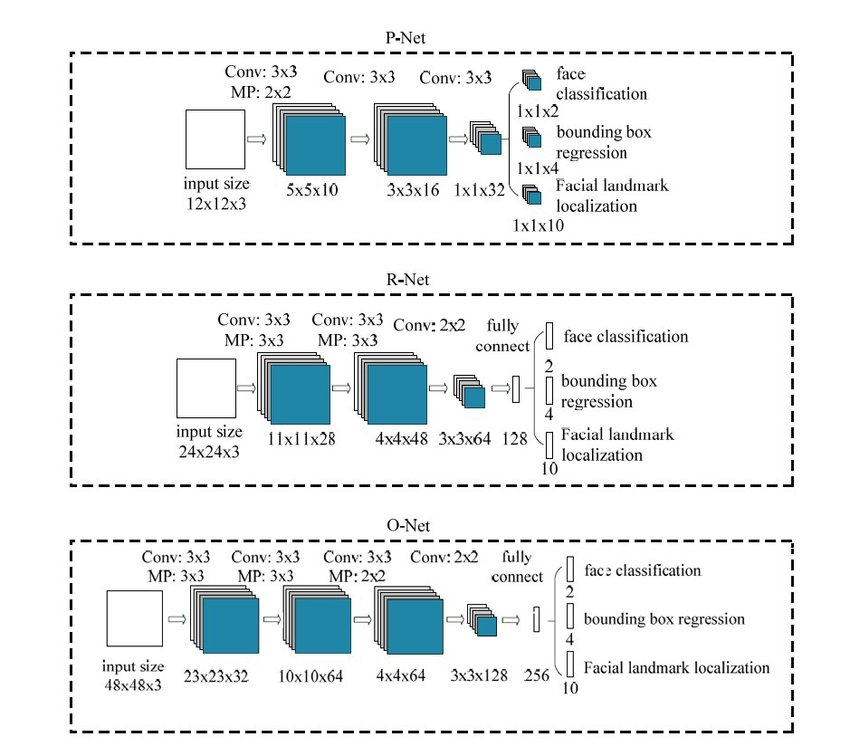
\includegraphics[width=1.\linewidth]{Chapters/items/chap2_9.jpg}
        \end{center}
        \label{fig: chap2_9}
    \end{subfigure}
    \caption{Các mạng neural trong MTCNN}
\end{figure}

\newpage
Với mỗi bức ảnh đầu vào, nó sẽ tạo ra nhiều bản sao của hình ảnh đó với các kích thước khác nhau.

Tại P-Net, thuật toán sử dụng 1 kernel 12x12 chạy qua mỗi bức hình để tìm kiếm khuôn mặt.

\begin{figure}
    \begin{subfigure}{1.\textwidth}
        \begin{center}
            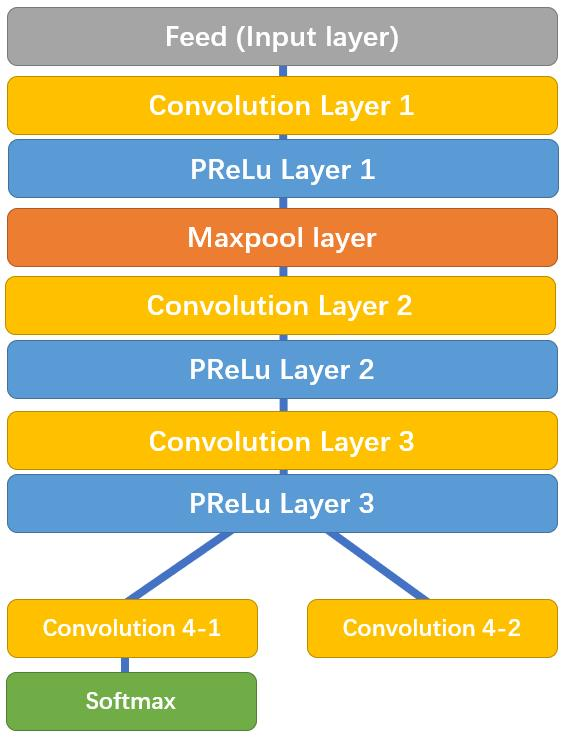
\includegraphics[width=0.6\linewidth]{Chapters/items/chap2_10.jpg}
        \end{center}
        \label{fig: chap2_10}
    \end{subfigure}
    \caption{Mô hình P-Net}
\end{figure}

\newpage
Sau lớp convolution thứ 3, mạng chia thành 2 lớp. Convolution 4-1 đưa ra xác suất của một khuôn mặt
nằm trong mỗi bounding boxes, và Convolution 4-2 cung cấp tọa độ của các bounding boxes.

R-Net có cấu trúc tương tự vói P-Net. Tuy nhiên sử dụng nhiều layer hơn.
Tại đây, network sẽ sử dụng các bounding boxes được cung cấp từ P-Net và tinh chỉnh là tọa độ.

\begin{figure}
    \begin{subfigure}{1.\textwidth}
        \begin{center}
            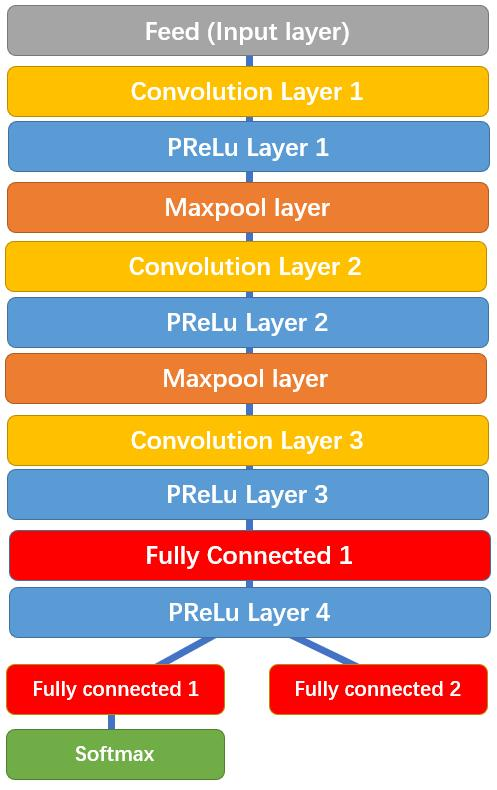
\includegraphics[width=0.6\linewidth]{Chapters/items/chap2_11.jpg}
        \end{center}
        \label{fig: chap2_11}
    \end{subfigure}
    \caption{Mô hình R-Net}
\end{figure}

\newpage
Tương tự R-Net chia ra làm 2 layers ở bước cuối, cung cấp 2 đầu ra đó là tọa độ
mới của các bounding boxes, cùng độ tin tưởng của nó.

O-Net lấy các bounding boxes từ R-Net làm đầu vào và đánh dấu các tọa độ của các mốc trên khuôn mặt.

\begin{figure}
    \begin{subfigure}{1.\textwidth}
        \begin{center}
            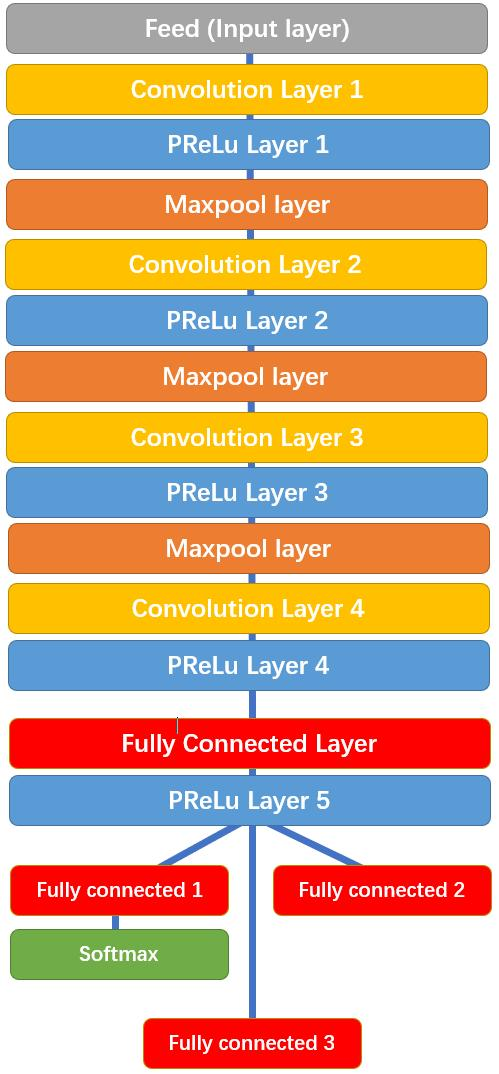
\includegraphics[width=0.55\linewidth]{Chapters/items/chap2_12.jpg}
        \end{center}
        \label{fig: chap2_12}
    \end{subfigure}
    \caption{Mô hình O-Net}
\end{figure}


Ở bước này, thuật toán đưa ra 3 kết quả đầu ra khác nhau bao gồm:
xác suất của khuôn mặt nằm trong bounding box, tọa độ của bounding box và
tọa độ của các mốc trên khuôn mặt (vị trí mắt, mũi, miệng)

\begin{figure}
    \begin{subfigure}{1.\textwidth}
        \begin{center}
            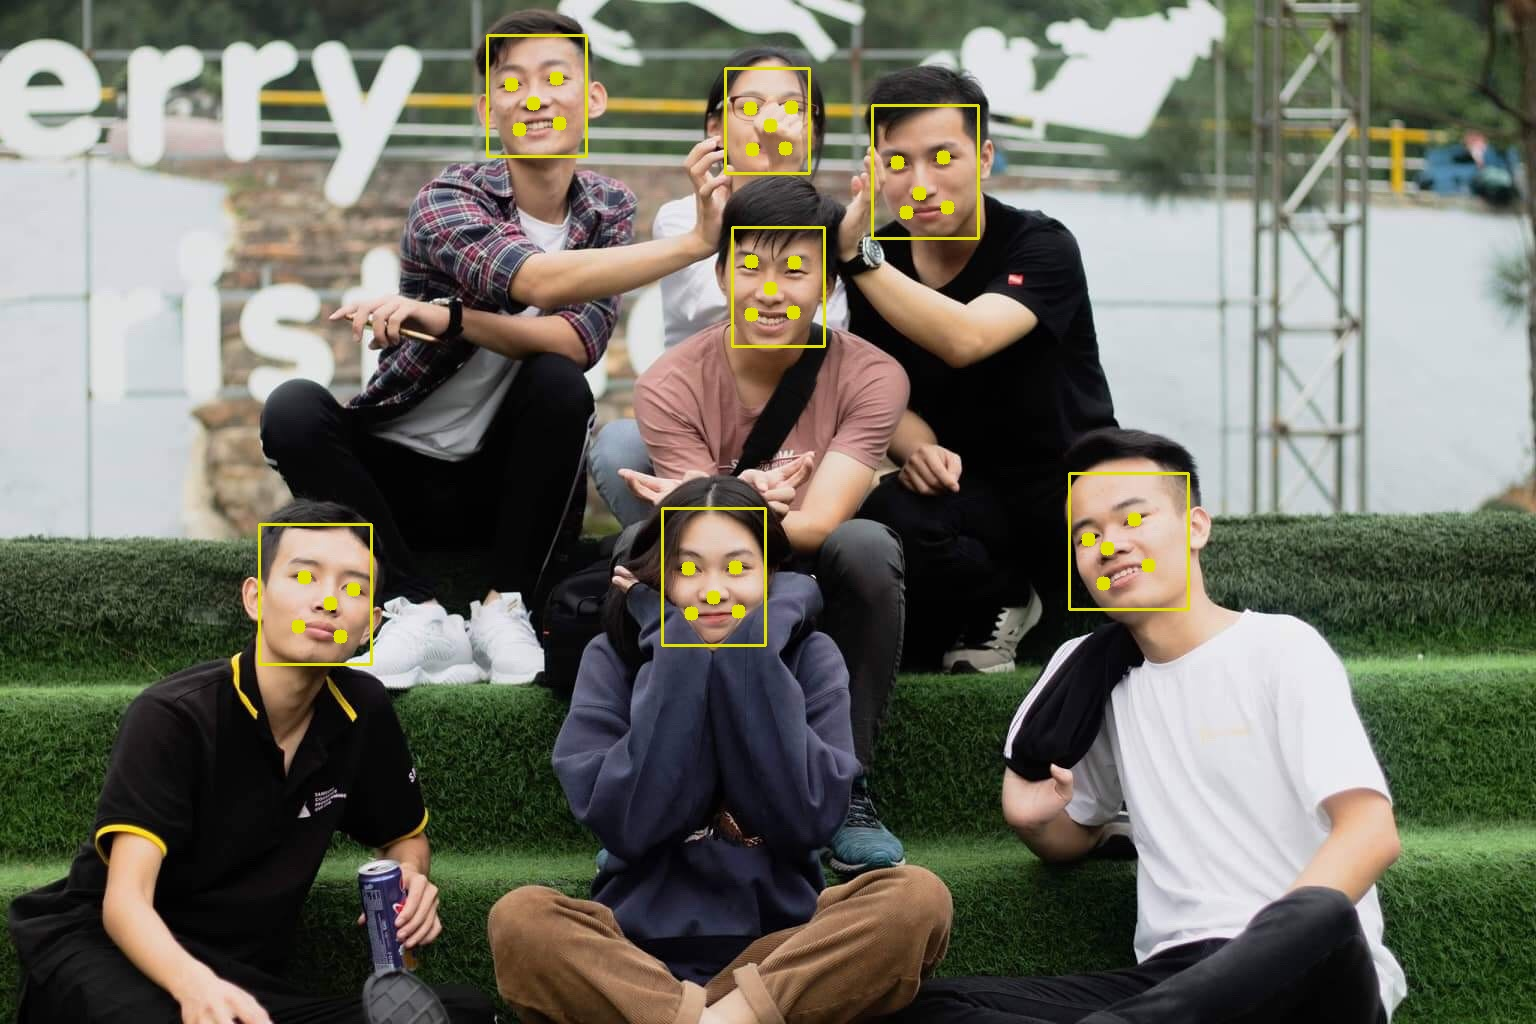
\includegraphics[width=1.\linewidth]{Chapters/items/chap2_14.jpg}
        \end{center}
        \label{fig: chap2_14}
    \end{subfigure}
    \caption{MTCNN xác định các khuôn mặt}
\end{figure}

\newpage
\section{Các kĩ thuật làm giàu dữ liệu (Data agumentation)}

Hiện nay các kĩ thuật làm giàu dữ liệu\cite{Augmentation} đang ngày các phát triển và phổ biến, khiến cho dữ liệu tăng lên
mạnh mẽ mà vẫn dữ được tính đặc trưng

Các kĩ thuật thường được sử dụng phổ biến là: Lật, xoay, phóng to, thu nhỏ, gây nhiễu, cắt, ...

Ngoài ra còn có các kĩ thuật nâng cao khác như là: sử dụng phép nội suy, GAN, đối xứng, bọc, ...

Còn rất nhiều những kĩ thuật phức tạp khác nhau và học sâu lại được sử dụng để giải quyết vấn đề này


\begin{figure}
    \begin{subfigure}{1.\textwidth}
        \begin{center}
            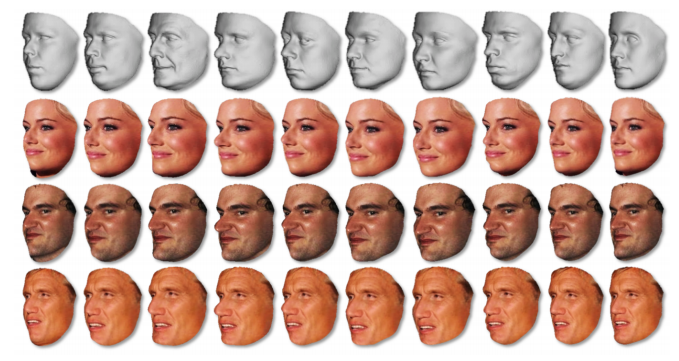
\includegraphics[width=1.\linewidth]{Chapters/items/chap3_6.jpg}
        \end{center}
        \label{fig: chap3_6}
    \end{subfigure}
    \caption{Làm giàu dữ liệu 3D sử dụng học sâu}
\end{figure}


\newpage
\section{Các thuật toán học sâu sử dụng trong nhận diện khuôn mặt}
\subsection{One-shot learning}

One-shot learning là thuật toán học có giám sát mà mỗi một người chỉ cần 1 vài,
rất ít hoặc thậm chí chỉ 1 bức ảnh duy nhất (để khỏi tạo ra nhiều biến thể).
Từ đầu vào là bức ảnh của một người, chúng ta sử dụng một kiến trúc CNN
đơn giản để dự báo người đó là ai.
Tuy nhiên nhược điểm của phương pháp này là chúng ta phải huấn luyện lại thuật
toán thường xuyên khi xuất hiện thêm một người mới vì số lượng của đầu ra thay đổi tăng lên 1.
Rõ ràng là không tốt đối với các hệ thống nhận diện khuôn mặt của một công ty vì số lượng người luôn biến động theo thời gian.

\subsection{Learning similarity}

Phương pháp này dựa trên một phép đo khoảng cách giữa 2 bức ảnh, thông thường là các định
mức chuẩn L1 hoặc L2 sao cho nếu 2 bức ảnh thuộc cùng một người thì khoảng cách là
nhỏ nhất và nếu không thuộc thì khoảng cách sẽ lớn hơn.

\begin{figure}
    \begin{subfigure}{0.8\textwidth}
        \begin{center}
            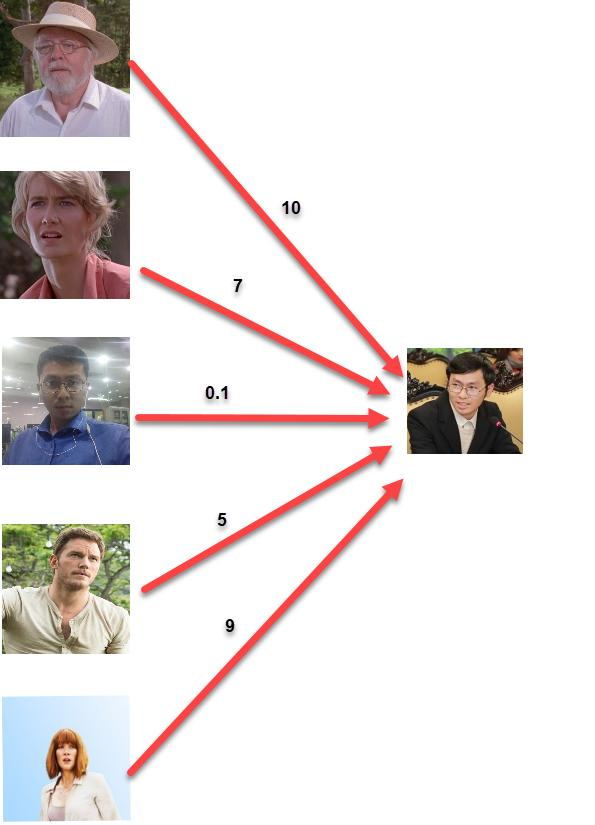
\includegraphics[width=0.5\linewidth]{Chapters/items/chap2_15.jpg}
        \end{center}
        \label{fig: chap2_15}
    \end{subfigure}
    \caption{Learning similarity}
\end{figure}
\newpage
Learning similarity có thể trả ra nhiều hơn một ảnh là cùng loại với ảnh đầu vào tùy theo ngưỡng (threshold).

Ngoài ra phương pháp này không bị phụ thuộc vào số lượng lớp (classes).
Do đó không cần phải huấn luyện lại khi xuất hiện class mới.
Điểm mấu chốt là cần xây dựng được một mô hình mã hóa (model encoding) đủ tốt để chiếu các bức
ảnh lên một không gian eucledean n chiều. Sau đó sử dụng khoảng cách để quyết
định nhãn của chúng.

Như vậy learning similarity có ưu điểm hơn so với one-shot learning khi không phải
huấn luyện lại model khi mà vẫn tìm ra được ảnh tương đồng.
Vậy làm thế nào để học được biểu diễn của ảnh trong không gian euledean n chiều?
Kiến trúc siam network sẽ giúp chúng ta thực hiện điều này một cách dễ dàng.

\subsection{Siam learning}

Những kiến trúc mạng mà khi bạn đưa vào 2 bức ảnh và mô hình sẽ trả lời chúng thuộc về
cùng 1 người hay không được gọi chung là Siam network.

Kiến trúc của Siam network dựa trên mạng cơ sở (base network) là một mạng neural tích chập (Convolutional neural network)
đã được loại bỏ các lớp đầu ra (output layer) có tác dụng mã hóa (encoding) ảnh thành vector nhúng (embedding).
Đầu vào của mạng siam network là 2 bức ảnh bất kì được lựa chọn ngẫu nhiên từ dữ liệu ảnh.
Output của Siam network là 2 vector tương ứng với biểu diễn của 2 ảnh đầu vào.
Sau đó đưa 2 vector vào hàm đánh giá mấy mát (loss function) để đo lường sự khác biệt giữa chúng.
Thông thường hàm đánh giá mất mát là một hàm chuẩn bậc 2.

\begin{figure}
    \begin{subfigure}{1.\textwidth}
        \begin{center}
            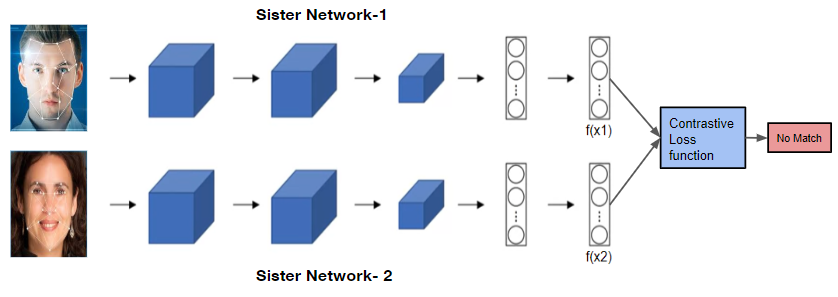
\includegraphics[width=1.\linewidth]{Chapters/items/chap2_16.jpg}
        \end{center}
        \label{fig: chap2_16}
    \end{subfigure}
    \caption{Siam learing}
\end{figure}

\newpage
Từ mô hình CNN, mô hình trả ra 2 vector mã hóa (encoding) là x1 và x2
biểu diễn cho lần lượt ảnh 1 và 2. x1 và x2 có cùng số chiều.
Hàm f(x) có tác dụng tương tự như một phép biến đổi qua lớp kết nối đầy đủ (layer fully connected)
trong mạng neural để tạo tính phi tuyến và giảm chiều dữ liệu về các kích thước nhỏ.
Thông thường là 128 đối đối với các mô hình đã được các nhà khoa học huấn luyện từ trước.

\begin{figure}
    \begin{subfigure}{1.\textwidth}
        \begin{center}
            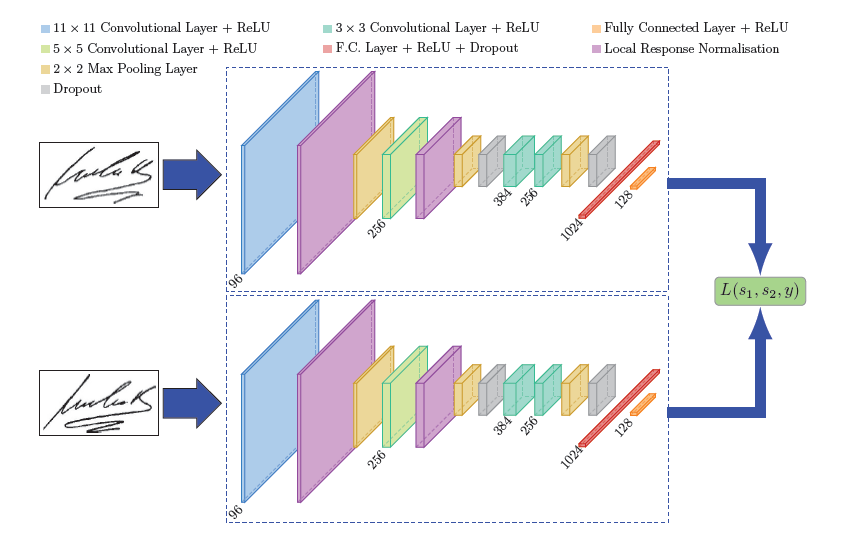
\includegraphics[width=1.\linewidth]{Chapters/items/siam.png}
        \end{center}
        \label{fig: siam}
    \end{subfigure}
    \caption{Siam network trong bài toán nhận dạng chữ ký}
\end{figure}


\newpage
\section{Mô hình học sâu được huấn luyện trước (Pre-train model)}
\subsection{Sử dụng mô hình được huấn luyện trước}

Mô hình huấn luyện trước là một mô hình được đào tạo bởi một người khác để giải quyết
một vấn đề tương tự. Thay vì xây dựng một mô hình từ đầu để giải quyết một vấn đề tương tự,
ta sử dụng mô hình được đào tạo về vấn đề khác làm điểm khởi đầu.
Thường thì những mô hình này là những mô hình rất lớn khó khăn trong việc huấn luyện
một mô hình được đào tạo trước có thể không chính xác 100\%,
nhưng nó giúp tiết kiệm rất nhiều thời gian và công sức.

\subsection{Giới thiệu Facenet}

FaceNet\cite{FaceNet} là một mạng lưới thần kinh sâu được sử dụng để trích xuất các tính năng từ
hình ảnh của một mặt người. Nó được xuất bản vào năm 2015 bởi các nhà nghiên cứu của Google.

\begin{figure}
    \begin{subfigure}{1.\textwidth}
        \begin{center}
            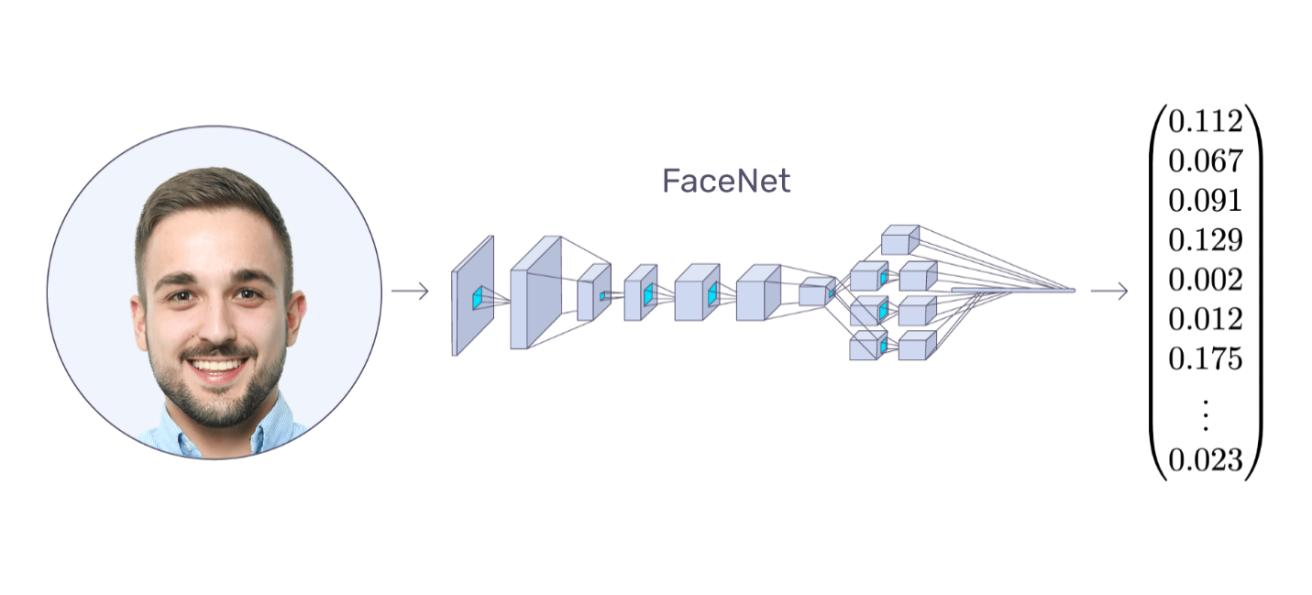
\includegraphics[width=1.\linewidth]{Chapters/items/chap2_17.jpg}
        \end{center}
        \label{fig: chap2_17}
    \end{subfigure}
    \caption{Facenet mã hóa hình ảnh khuôn mặt thành vector 128 chiều}
\end{figure}

FaceNet lấy hình ảnh của mặt người làm đầu vào và xuất ra một vector 128 chiều,
đại diện cho các tính năng quan trọng nhất của khuôn mặt.
Trong học máy, vector này được gọi là nhúng (embeddings).
Tại sao phải nhúng? Bởi vì tất cả các thông tin quan trọng từ một hình ảnh được nhúng
vào vector này. Về cơ bản, FaceNet lấy một mặt người và nén nó thành một vector gồm 128 số.
Khuôn mặt cần định danh cũng có nhúng tương tự.

Facenet chính là một dạng siam network có tác dụng biểu diễn các bức ảnh trong một không
gian eucledean n chiều (thường là 128) sao cho khoảng cách giữa các vector nhúng(embedding)
càng nhỏ, mức độ tương đồng giữa chúng càng lớn.

Hầu hết các thuật toán nhận diện khuôn mặt trước facenet đều tìm cách biểu diễn
khuôn mặt bằng một vector nhúng (embedding) thông qua một layer bottle neck có tác dụng
giảm chiều dữ liệu:

\begin{itemize}
    \item Tuy nhiên hạn chế của các thuật toán này đó là số lượng chiều vector nhúng (embedding)
          tương đối lớn (thường >= 1000) và ảnh hưởng tới tốc độ của thuật toán.
          Thường chúng ta phải áp dụng thêm thuật toán PCA để giảm chiều dữ liệu để giảm
          tốc độ tính toán.
    \item Hàm đánh giá mất mát (loss function) chỉ đo lường khoảng cách giữa 2 bức ảnh.
          Như vậy trong một đầu vào huấn luyện chỉ học được một trong hai khả năng
          là sự giống nhau nếu chúng cùng 1 lớp hoặc sự khác nhau nếu chúng khác
          lớp mà không học được cùng lúc sự giống nhau và khác nhau trên cùng một
          lượt huấn luyện.
\end{itemize}

Facenet đã giải quyết cả 2 vấn đề trên bằng các hiệu chỉnh nhỏ nhưng mang lại hiệu quả lớn:

\begin{itemize}
    \item Mạng cơ sở áp dụng một mạng neural tích chập và giảm chiều dữ
          liệu xuống chỉ còn 128 chiều. Do đó quá trình suy diễn và dự báo nhanh hơn và
          đồng thời độ chính xác vẫn được đảm bảo.
    \item Sử dụng hàm đánh giá mất mát là hàm đánh giá bộ ba (triplet loss) có khả năng học được đồng thời
          sự giống nhau giữa 2 bức ảnh cùng nhóm và phân biệt các bức ảnh không cùng nhóm.
          Do đó hiệu quả hơn rất nhiều so với các phương pháp trước đây.
\end{itemize}

\newpage
\subsection{Giới thiệu Mạng InceptionResnetV1}

Mạng InceptionResnetV1\cite{resnet} có là sự kết hợp giữa 2 mạng cơ sở là InceptionNet hay còn gọi là GoogLe Net và ResNet.

Nó được giới thiệu năm 2016 bởi các kĩ sư của Google, và cho thấy hiệu quả mạnh mẽ trên những tập dữ liệu ảnh lớn
tiêu biểu là tập dữ liệu ImageNet.

\begin{figure}
    \begin{subfigure}{1.\textwidth}
        \begin{center}
            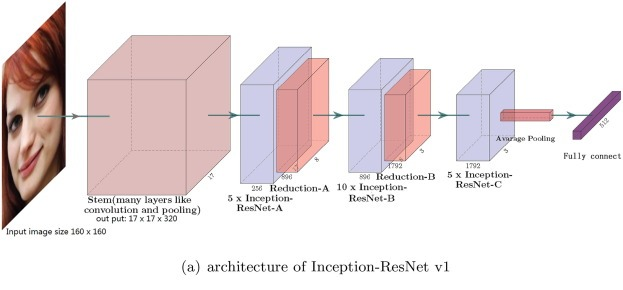
\includegraphics[width=1.\linewidth]{Chapters/items/chap2_19.jpg}
        \end{center}
        \label{fig: chap2_19}
    \end{subfigure}
    \caption{Cấu trúc tổng quan của InceptionResnetV1}
\end{figure}

InceptionResnetV1 là một mạng CNN kết hợp giữa các cấu trúc lớn với khoảng 23 triệu tham số trong mạng đồng nghĩa với
mỗi khi cho ảnh đi qua mạng này phải thực hiện 23 triệu phép tính, còn chưa kể trong quá trình huẩn luyện
mạng này phải thực hiện rất nhiều phép tính để thay đổi các tham số.

Chính vì sự khổng lồ của nó nên đã gây ra sự khó khăn trong quá trình huấn luyện, với những điều kiện như:
lượng dữ liệu cho huấn luyện phải thật sự lớn (lên tới hàng chục triệu ảnh với hàng triệu khuôn mặt),
phần cứng hỗ trợ tính toán tốn kém, tài nguyên lưu trữ lớn, ...

Rất may mắn rằng có các tổ chức với lợi thế về dữ liệu, tài nguyên phần cứng đã huấn luyện thành công
các mạng này với những kết quả có độ chính xác cực cao.

Nên tôi đã sử dụng InceptionResnetV1 làm mạng cơ sở cho hệ thống này

\newpage
\subsection{Kĩ thuật đánh giá bộ ba (Triplet loss)}
Trong Facenet, quá trình mã hóa của CNN đã giúp ta mã hóa bức ảnh về 128 chiều.
Sau đó những vector này sẽ làm đầu vào cho hàm đánh giá bộ ba để đánh giá khoảng
cách giữa các vector.

\begin{figure}
    \begin{subfigure}{1.\textwidth}
        \begin{center}
            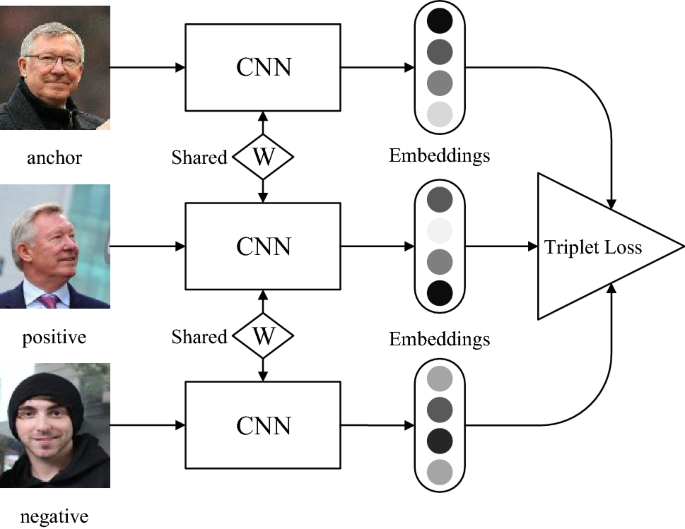
\includegraphics[width=1.\linewidth]{Chapters/items/chap2_18.jpg}
        \end{center}
        \label{fig: chap2_18}
    \end{subfigure}
    \caption{Mô hình sử dụng hàm đánh giá bộ ba}
\end{figure}

Mục tiêu của triplet loss là đảm bảo rằng:
\begin{itemize}
    \item Hai ví dụ có cùng nhãn có các phần nhúng của chúng gần nhau trong không gian nhúng.
    \item Hai ví dụ với các nhãn khác nhau có các nhúng của chúng ở xa nhau.
\end{itemize}

Để áp dụng triple loss, chúng ta cần lấy ra 3 bức ảnh trong đó có một bức ảnh là anchor.
Trong 3 ảnh thì ảnh anchor được cố định trước.
Chúng ta sẽ lựa chọn 2 ảnh còn lại sao cho một ảnh là negative
(của một người khác với anchor) và một ảnh là positive (cùng một người với anchor).


Mục tiêu của hàm triplet loss là tối thiểu hóa khoảng cách giữa 2 ảnh khi chúng là
negative và tối đa hóa khoảng cách khi chúng là positive.
Như vậy chúng ta cần lựa chọn các bộ 3 ảnh sao cho:
\begin{itemize}
    \item Ảnh Anchor và Positive khác nhau nhất: cần lựa chọn để khoảng cách d(A,P) lớn.
          Điều này cũng tương tự như bạn lựa chọn một ảnh của mình hồi nhỏ so với hiện tại để
          thuật toán học khó hơn. Nhưng nếu nhận biết được thì nó sẽ thông minh hơn.
    \item Ảnh Anchor và Negative giống nhau nhất: cần lựa chọn để khoảng cách d(A,N)
          d(A,N) nhỏ. Điều này tương tự như việc thuật toán phân biệt được ảnh của một người
          anh em giống bạn.
\end{itemize}

\begin{figure}
    \begin{subfigure}{0.8\textwidth}
        \begin{center}
            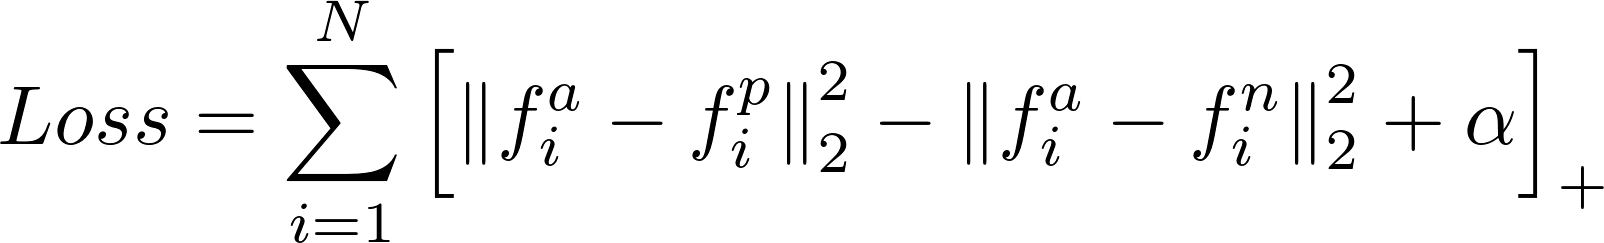
\includegraphics[width=1.\linewidth]{Chapters/items/fomura.png}
        \end{center}
        \label{fig: fomura}
    \end{subfigure}
    \caption{Công thức của hàm đánh giá bộ ba}
\end{figure}



%!TEX root = ../../book_ML.tex
\chapter{Thiết kế và xây dựng hệ thống}
\label{cha:chap3}
% \index{principal component analysis}
% \index{PCA -- \textit{xem} principle component analysis}
% \index{PCA}

% \index{phân tích thành phần chính -- principle component analysis}
% \index{principle component analysis -- phân tích thành phần chính}
% \index{PCA}
\section{Phân tích}
Về cơ bản một hệ thống điểm danh bằng khuôn mặt gồm các bước sau:
\begin{itemize}
    \item Thu thập dữ liệu khuôn mặt
    \item Phát hiện khuôn mặt dựa trên ảnh đầu vào và gán nhãn dữ liệu
    \item Làm giàu dữ liệu
    \item Trích xuất các đặc trưng (sử dụng học sâu)
    \item Đưa các đặc trưng đã được gán nhãn vào thuật toán phân loại
    \item Lưu trữ các thông tin và kết quả phân loại đã được học
    \item Nhận dạng khuôn mặt
\end{itemize}

\section{Xây dựng}
%!TEX root = ../../book_ML.tex
\chapter{Kết luận và hướng phát triển}
\label{cha:chap4}

\section{Kết luận}
Trên cơ sở tìm hiểu về bài toán nhận diện mặt người trong ảnh, sử dụng pre-trained
model FaceNet được huấn luyện trước trên mạng cơ sở là InceptionResnetV1 do
tiến sĩ khoa học máy tính David Sandberg cung cấp, tôi đã xây dựng thành công hệ
thống điểm danh thông qua hình ảnh khuôn mặt.

Về khả năng phát hiện khuôn mặt, kết quả phát hiện khá tốt hầu hết các trường hợp,
kể cả trong điều kiện thiếu sáng, góc nghiêng, hay có vật che khuất như kính mắt,…

Về khả năng nhận dạng, hệ thống đạt kết quả từ 96-98\% đối với các khuôn mặt thẳng
và điều kiện ánh sáng thích hợp, đạt 92-95\% đối với các khuôn mặt nghiêng hoặc
thiếu sáng.

Về khả năng loại trừ các khuôn mặt “unknown face”, kết quả đạt khoảng 85-90\% khuôn mặt lạ
được phát hiện trong quá trình thử nghiệm.
Hệ thống điểm danh hoạt động ổn định và mượt mà nhờ máy chủ viết bằng Python.
Giao diện được xây dựng trên nền Web là một lợi thế vì tính đơn giản và tiện lợi.

\section{Hướng phát triển}

Dựa trên những cơ sở sẵn có này thệ thống có thể được cải tiến trong
tương lai bằng những phương pháp sau:
\begin{itemize}
    \item Cải thiện thời gian chạy của hệ thống, nâng cấp lên có thể chạy trong thời gian thực
    \item Để cải thiện độ chính xác cho hệ thống, đầu tiên ta cần cải thiện bộ dữ liệu dựa trên các tiêu chí như tư thế chụp, góc chụp, hạn chế sự che khuất các bộ phận trên mặt, biểu cảm khuôn mặt, điều kiện ánh sáng, tuổi tác…
    \item Thử nghiệm với nhiều mô hình được huấn luyện trước và thuật toán huấn luyện khác nhau cho bộ dữ liệu của hệ thống.
    \item Thay thế phương pháp loại bỏ khuôn mặt lạ, thử nghiệm và chọn ra ngưỡng cho phép phù hợp hơn.
\end{itemize}

Không chỉ dừng lại ở việc điểm danh, của hệ thống nhận dạng khuôn mặt có thể được sử dụng trong các 
hệ thống mở khóa, thanh toán, hay truy tìm tội phạm,…




% %!TEX root = ../../book_ML.tex
\chapter{Phân tích thành phần chính}
\label{cha:pca}
% \index{principal component analysis}
% \index{PCA -- \textit{xem} principle component analysis}
\index{PCA}

\index{phân tích thành phần chính -- principle component analysis}
\index{principle component analysis -- phân tích thành phần chính}
\index{PCA}
\section{Phân tích thành phần chính}
\subsection{Ý tưởng} % (fold)


% subsection ý_tưởng (end)
%%%%%%% Three subfigures with bottom caption%%%%%%%%%%%%%%
\begin{figure}[t]
    \begin{subfigure}{0.59\textwidth}
        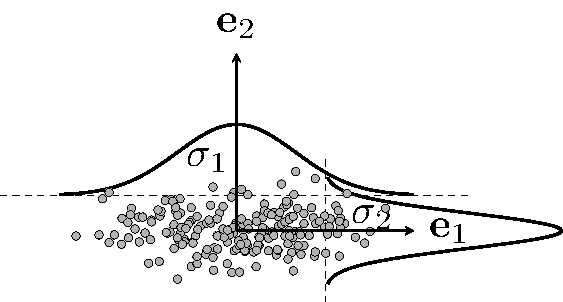
\includegraphics[width=0.99\linewidth]{Chapters/content/27_pca/latex/pca_diagvar.pdf}
        \caption{}
        \label{fig:pca_2a}
    \end{subfigure}
    \begin{subfigure}{0.33\textwidth}
        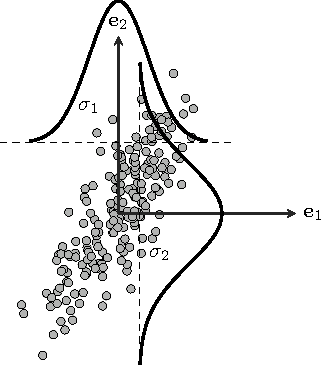
\includegraphics[width=0.99\linewidth]{Chapters/content/27_pca/latex/pca_var0.pdf}
        \caption{}
        \label{fig:pca_2b}
    \end{subfigure}
    \caption{Ví dụ về phương sai của dữ liệu trong không gian hai chiều. (a)
        Phương sai của chiều thử hai (tỉ lệ với độ rộng của đường hình chuông) nhỏ
        hơn phương sai của chiều thứ nhất. (b) Cả hai chiều có phương sai đáng kể. Phương sai của
        mỗi chiều là phương sai của thành phần tương ứng được lấy trên toàn bộ dữ
        liệu. Phương sai tỉ lệ thuận với độ phân tán của dữ liệu.}
    \label{fig:pca_2}
\end{figure}

Giả sử vector dữ liệu ban đầu $\bx \in \R^{D}$ được giảm chiều trở thành $\bz
    \in \R^K$ với $K < D$. Một cách đơn giản để giảm chiều dữ liệu từ $D$ về $K < D$ là chỉ giữ lại $K$ phần tử {quan trọng nhất}. Có hai câu hỏi lập tức
được đặt ra. Thứ nhất, làm thế nào để xác định {tầm quan trọng} của
mỗi phần tử? Thứ hai, nếu tầm quan trọng của các phần tử là như
nhau, ta cần bỏ đi những phần tử nào?

Để trả lời câu hỏi thứ nhất, hãy quan sát Hình~\ref{fig:pca_2a}. Giả sử các
điểm dữ liệu có thành phần thứ hai (phương đứng) giống hệt nhau hoặc sai khác
nhau không đáng kể (phương sai nhỏ). Khi đó, thành phần này hoàn toàn có thể được lược
bỏ, và ta ngầm hiểu rằng nó sẽ được xấp xỉ bằng kỳ vọng của thành phần đó
trên toàn bộ dữ liệu. Ngược lại, nếu áp dụng phương pháp này lên chiều thứ nhất (phương ngang), {lượng thông tin} bị mất đi đáng kể do sai số xấp xỉ quá lớn. Vì vậy, lượng thông tin theo mỗi thành phần có thể được đo bằng phương sai của dữ liệu trên thành phần đó. Tổng lượng
thông tin là tổng phương sai trên toàn bộ các thành phần. Lấy
một ví dụ về việc có hai camera được đặt dùng để chụp cùng một người, một camera
phía trước và một camera đặt trên đầu. Rõ ràng, hình ảnh thu được từ
camera đặt phía trước mang nhiều thông tin hơn so với hình ảnh nhìn từ
phía trên đầu. Vì vậy, bức ảnh chụp từ phía trên đầu có thể được bỏ qua mà không
làm mất đi quá nhiều thông tin về hình dáng của người đó.

Câu hỏi thứ hai tương ứng với trường hợp Hình~\ref{fig:pca_2b}. Trong cả hai
chiều, phương sai của dữ liệu đều lớn; việc bỏ đi một trong hai chiều đều khiến
một lượng thông tin đáng kể bị mất đi. Tuy nhiên, nếu xoay trục toạ độ đi một
góc phù hợp, một trong hai chiều dữ liệu có thể được lược bở vì dữ liệu có xu
hướng phân bố xung quanh một đường thẳng.

\textit{Phân tích thành phần chính} (principle component analysis, PCA) là
phương pháp đi tìm một phép xoay trục toạ độ để được một hệ trục toạ độ mới sao
cho trong hệ mới này, thông tin của dữ liệu chủ yếu tập trung ở một vài thành
phần. Phần còn lại chứa ít thông tin hơn có thể được lược bỏ.

Phép xoay trục toạ độ có liên hệ chặt chẽ tới hệ trực chuẩn và ma trận trực giao
.Giả sử hệ cơ sở trực chuẩn mới là $\bU$ (mỗi cột của $\bU$ là một vector đơn vị cho
một chiều) và ta muốn giữ lại $K$ toạ độ trong hệ
cơ sở mới này. Không mất tính tổng quát, giả sử đó là $K$ thành phần đầu tiên.
% ******************************************************************************
\begin{figure}[t]
    \centering
    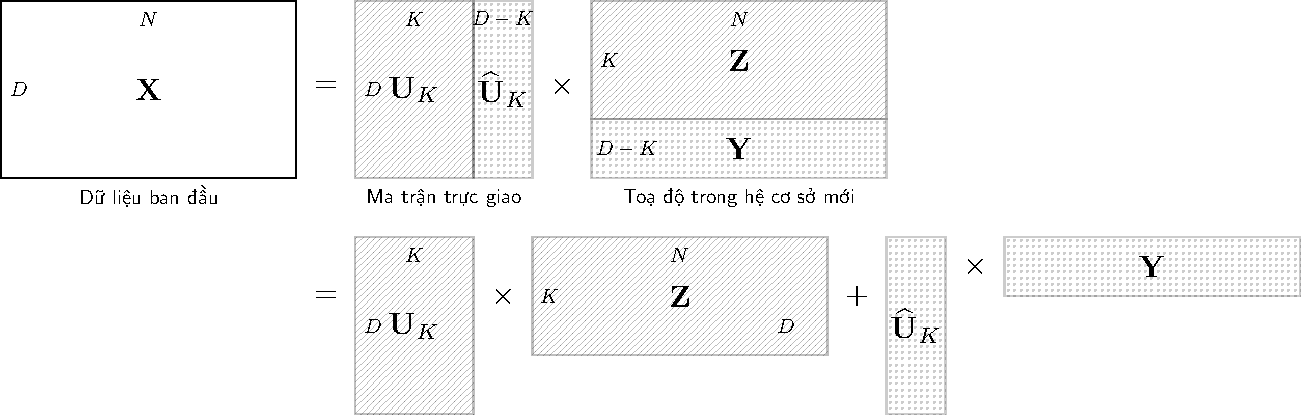
\includegraphics[width = \textwidth]{Chapters/content/27_pca/latex/pca_idea.pdf}
    \caption[]{Ý tưởng chính của PCA: Tìm một hệ trực chuẩn mới sao cho trong hệ này, các thành phần quan trọng nhất nằm trong $K$ thành phần đầu tiên.}
    \label{fig:27_3}
\end{figure}
% ******************************************************************************
Quan sát Hình~\ref{fig:27_3} với cơ sở mới $\bU =
    [\bU_K, \what{\bU}_K]$ là một hệ trực chuẩn với $\bU_K$ là ma trận con tạo bởi $K$ cột đầu tiên của $\bU$. Trong hệ cơ sở mới này, ma trận dữ liệu có thể được viết thành
\begin{equation}
    \label{eqn:27_8}
    \bX = \bU_K \mathbf{Z} + \widehat{\bU}_K \mathbf{Y}
\end{equation}
Từ đây ta cũng suy ra
\begin{eqnarray}
    \label{eqn:27_9}
    \left[\begin{matrix} \mathbf{Z} \\\ \mathbf{Y} \end{matrix} \right] =
    \left[\begin{matrix} \bU_K^T \\\ \what{\bU}_K^T \end{matrix} \right]\bX \Rightarrow
    \begin{matrix}
        \mathbf{Z} = \bU_K^T \bX \\\
        \mathbf{Y} = \what{\bU}_K^T\bX
    \end{matrix}
\end{eqnarray}
Mục đích của PCA là đi tìm ma trận trực giao $\bU$ sao cho phần lớn thông tin
nằm ở $\bU_K \mathbf{Z}$, phần nhỏ thông tin nằm ở $\what{\bU}_K\mathbf{Y}$.
Phần nhỏ này sẽ được lược bỏ và xấp xỉ bằng một ma trận có các
cột như nhau. Gọi mỗi cột đó là
$\mathbf{b}$, khi đó, ta sẽ xấp xỉ $\mathbf{Y} \approx
    \mathbf{b1}^T$ với $\mathbf{1}^T\in \mathbb{R}^{1
        \times N}$ là một vector hàng có toàn
bộ các phần tử bằng một. Giả sử đã tìm được $\bU$, ta cần tìm $\mathbf{b}$ thoả mãn:
\begin{equation}
    \mathbf{b} = \text{argmin}_{\bb} \|\mathbf{Y} - \mathbf{b1}^T\|_F^2 =
    \text{argmin}_{\mathbf{b}} \|\what{\bU}_K^T\bX - \mathbf{b1}^T\|_F^2
\end{equation}
Giải phương trình đạo hàm theo $\mathbf{b}$ của hàm mục tiêu bằng $\bzero$:
\begin{equation}
    (\mathbf{b1}^T - \what{\bU}_K^T\bX)\mathbf{1} = 0 \Rightarrow N\mathbf{b} = \what{\bU}_K^T \mathbf{X1} \Rightarrow \mathbf{b} = \what{\bU}_K^T \lbar{\mathbf{x}}.
\end{equation}
Ở đây ta đã sử dụng $\bone^T\bone = N$ và $\lbar{\bx} = \frac{1}{N}\bX\bone$ là
vector trung bình các cột của $\bX$.
Với giá trị $\mathbf{b}$ tìm được này, dữ liệu ban đầu sẽ được xấp xỉ bởi
\begin{equation}
    \label{eqn:27_10}
    \bX = \bU_K \bZ + \what{\bU}_k\bY \approx \bU_K\bZ + \what{\bU}_k \bb\bone^T
    = \bU_K \mathbf{Z} + \what{\bU}_K \what{\bU}_K^T\bar{\mathbf{x}}\mathbf{1}^T
    \triangleq \tilde{\bX}
    % \bX \approx \tilde{\bX} = \bU_K \mathbf{Z} + \what{\bU}_K \what{\bU}_K^T\bar{\mathbf{x}}\mathbf{1}^T
\end{equation}
\subsection{Hàm mất mát}
Hàm mất mát của PCA được coi như sai số của phép xấp xỉ, được định
nghĩa là
\begin{eqnarray}
    \nonumber
    \frac{1}{N}\|\bX - \tilde{\bX}\|_F^2 &=&
    \frac{1}{N}\|\what{\bU}_K \bY-  \what{\bU}_K
    \what{\bU}_K^T\lbar{\bx}\bone^T\|_F^2 =
    \frac{1}{N}\|\what{\bU}_K \what{\bU}_K^T \bX -  \what{\bU}_K
    \what{\bU}_K^T \bar{\mathbf{x}}\mathbf{1}^T\|_F^2\\
    \label{eqn:27_11}
    &=& \frac{1}{N} \|\what{\bU}_k \what{\bU}_k^T(\bX - \lbar{\bx}\bone^T)\|_F^2
    \triangleq J(\bU)
\end{eqnarray}
Chú ý rằng, nếu các cột của một ma trận $\mathbf{V}$ tạo thành một hệ
trực chuẩn thì với một ma trận $\mathbf{W}$ bất kỳ, ta luôn có
\begin{equation}
    \|\mathbf{VW}\|_F^2 = \text{trace} (\mathbf{W}^T\mathbf{V}^T\mathbf{V} \mathbf{W}) = \text{trace}(\mathbf{W}^T\mathbf{W}) = \|\mathbf{W}\|_F^2
\end{equation}
Đặt $\what{\bX} = \bX - \lbar{\bx}\bone^T$. Ma trận này có được bằng cách trừ
mỗi cột của $\bX$ đi trung bình các cột của nó. Ta gọi $\what{\bX}$ là {ma trận dữ liệu đã
được chuẩn hoá}. Có thể thấy $\hat{\mathbf{x}}_n = \mathbf{x}_n -
    \bar{\mathbf{x}},~\forall n = 1, 2, \dots, N$.

% Ta tạm gọi
% $\what{\bX}$ là ma trận dữ liệu chuẩn hoá.

Vì vậy hàm mất mát trong~\eqref{eqn:27_11} có thể được viết lại thành:
\begin{eqnarray}
    J(\bU) &=&  \frac{1}{N} \|\what{\bU}_K^T\what{\bX} \|_F^2 = \frac{1}{N}
    \|\what{\bX}^T \what{\bU}_K \|_F^2 =
    \frac{1}{N}\sum_{i = K+1}^D \|\what{\bX}^T\mathbf{u}_i \|_2^2 \\\
    \label{eqn:27_12}
    &=& \frac{1}{N} \sum_{i=K+1}^D \mathbf{u}_i^T\what{\bX}\what{\bX}^T \mathbf{u}_i
    = \sum_{i=K+1}^D \mathbf{u}_i^T\mathbf{S} \mathbf{u}_i
\end{eqnarray}
với $\mathbf{S} = \frac{1}{N}\what{\bX}\what{\bX}^T$ là ma trận hiệp phương sai
của dữ liệu và luôn là một ma trận nửa xác định dương.
% (xem Mục~\ref{sub:expectaion_covariance}).

Công việc còn lại là tìm các $\mathbf{u}_i$ để mất mát là nhỏ nhất.

Với ma trận $\bU$ trực giao bất kỳ, thay $K = 0$ vào \eqref{eqn:27_12} ta có
\begin{eqnarray}
    L &=& \sum_{i=1}^D \mathbf{u}_i^T\mathbf{Su}_i = \frac{1}{N} \|\what{\bX}^T\bU\|_F^2 =\frac{1}{N} \text{trace}(\what{\bX}^T\bU \bU^T \what{\bX})  \\\
    \label{eqn:27_13}
    &=& \frac{1}{N} \text{trace} (\what{\bX}^T \what{\bX})  = \frac{1}{N} \text{trace} (\what{\bX} \what{\bX}^T) =\text{trace} (\mathbf{S}) = \sum_{i=1}^D \lambda_i
\end{eqnarray}
Với $\lambda_1 \geq \lambda_2 \geq \dots \geq \lambda_D \geq 0$ là các trị riêng
của ma trận nửa xác định dương $\mathbf{S}$. Chú ý rằng các trị riêng này là
thực và không âm\footnote{Tổng các trị riêng của một ma trận vuông bất kỳ luôn
    bằng vết của ma trận đó.}.


\textit{Như vậy $L$ không phụ thuộc vào cách chọn ma trận trực giao $\bU$} và
bằng tổng các phần tử trên đường chéo của $\mathbf{S}$. Nói cách khác, $L$ chính
là tổng các phương sai theo từng thành phần của dữ liệu ban
đầu\footnote{Mỗi thành phần trên đường chéo chính của ma trận hiệp phương sai
    chính là phương sai của thành phần dữ liệu tương ứng.}.

Vì vậy, việc tối thiểu hàm mất mát $J$ được cho bởi \eqref{eqn:27_12} tương
đương với việc tối đa biểu thức
\begin{equation}
    F  = L - J = \sum_{i=1}^K \mathbf{u}_i \mathbf{S} \mathbf{u}_i^T
\end{equation}
\subsection{Tối ưu hàm mất mát}
Nghiệm của bài toán tối ưu hàm mất mát PCA được tìm dựa trên khẳng định sau
đây:
\newnote{}{
    Nếu $\bS$ là một ma trận nửa xác định dương, bài toán tối ưu
    \begin{eqnarray}
        \max_{\bU_K} \sum_{i=1}^K \bu_i^T\bS\bu_i \\
        \text{thoả mãn:}~ \bU_K^T\bU_K = \bI
    \end{eqnarray}
    có nghiệm $\bu_1, \dots, \bu_K$ là các vector riêng ứng với $K$ trị riêng (kể
    cả lặp) lớn
    nhất của $\bS$. Khi đó, giá trị lớn nhất của hàm mục tiêu là $\sum_{i=1}^K\lambda_i$, với
    $\lambda_1 \geq \lambda_2 \geq \dots \geq \lambda_D$ là các trị riêng của $\bS$.
}

% \textbf{Định lý 1:} $F$ đạt giá trị lớn nhất bằng $\sum_{i=1}^K \lambda_i$ khi $\mathbf{u}_i$ là các vector riêng có norm 2 bằng 1 ứng với các trị riêng này. Tất nhiên, chúng ta không quên điều kiện trực giao giữa các $\mathbf{u}_i$.

% Chú ý rằng $\lambda_i, i = 1, \dots, K$ chính là $K$ trị riêng lớn nhất của ma trận hiệp phương sai $\mathbf{S}$.
Khẳng định này có thể được chứng minh bằng quy nạp
% \footnote
% {Xin được bỏ qua
% phần chứng minh. Bạn đọc có thể xem Excercise 12.1 trong tài liệu tham
% khảo~\cite{bishop2006pattern} với lời giải tại \url{https://goo.gl/sM32pB}.}.

Trị riêng lớn nhất $\lambda_1$ của ma trận hiệp phương sai $\bS$ còn được gọi
là \textit{thành
    phần chính thứ nhất} ({the first principal component}), trị riêng thứ hai
$\lambda_2$ được gọi là \textit{thành phần chính thứ hai},... Tên gọi
\textit{phân tích thành phần chính} ({principal component analysis}) bắt
nguồn từ đây. Ta chỉ giữ lại $K$ thành phần chính đầu tiên khi giảm chiều dữ
liệu dùng PCA.

% ******************************************************************************
\begin{figure}[t]
    % caption on side


    \floatbox[{\capbeside\thisfloatsetup{capbesideposition={right,top},capbesidewidth=7.5cm}}]{figure}[\FBwidth]
    {\caption{ PCA có thể được coi là phương pháp đi tìm một hệ cơ sở trực chuẩn
            đóng vai trò một phép xoay, sao cho trong hệ cơ sở mới này, phương sai theo
            một số chiều nào đó là không đáng kể và có thể lược bỏ. Trong hệ cơ sở ban đầu
            $\mathbf{O}\be_1\be_2$, phương sai theo mỗi chiều (độ rộng của các đường
            hình chuông nét liền) đều lớn. Trong không gian mới với hệ cơ sở
            $\mathbf{O}\bu_1\bu_2$, phương sai theo hai chiều (độ rộng của các đường
            hình chuông nét đứt) chênh lệch nhau đáng kể. Chiều dữ liệu có phương sai nhỏ
            có thể được lược bỏ vì dữ liệu theo chiều này ít phân tán. }
        \label{fig:27_4}}
    { % figure here

        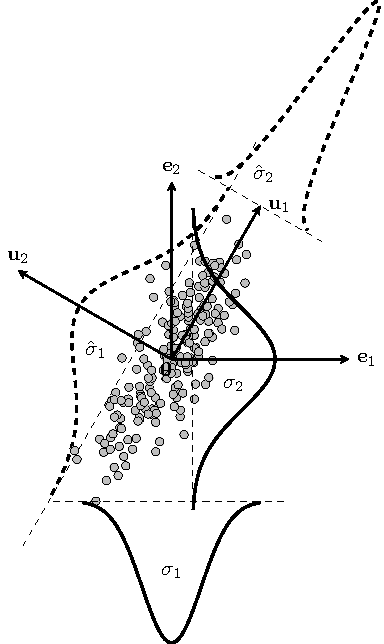
\includegraphics[width=.4\textwidth]{Chapters/content/27_pca/latex/pca_var.pdf}
    }
\end{figure}
% ******************************************************************************
Hình~\ref{fig:27_4} minh hoạ các thành phần chính với dữ liệu hai chiều.
Trong không gian ban đầu với các vector cơ sở $\mathbf{e}_1,
    \mathbf{e}_2$, phương sai theo mỗi chiều dữ liệu (tỉ lệ với độ rộng của các hình chuông
nét liền) đều lớn. Trong hệ cơ sở mới $\mathbf{O}\mathbf{u}_1\mathbf{u}_2$,
phương sai theo chiều thứ hai $\hat{\sigma}_2^2$ nhỏ so với
$\hat{\sigma}_1^2$. Điều này chỉ ra rằng khi chiếu dữ liệu lên $\mathbf{u}_2$, ta
được các điểm rất gần nhau và gần với giá trị trung bình theo chiều đó. Trong
trường hợp này, vì giá trị trung bình theo mọi chiều bằng 0, ta có thể thay thế
toạ độ theo chiều $\mathbf{u}_2$ bằng 0. Rõ ràng là nếu dữ liệu có phương sai
càng nhỏ theo một chiều nào đó thì khi xấp xỉ chiều đó bằng một hằng số, sai số
xấp xỉ càng nhỏ. PCA thực chất là đi tìm một phép xoay tương ứng với một ma trận
trực giao sao cho trong hệ toạ độ mới, tồn tại các chiều có phương sai nhỏ
có thể được bỏ qua; ta chỉ cần giữ lại các chiều/thành phần khác quan trọng hơn. Như
đã khẳng định ở trên, tổng phương sai theo toàn bộ các chiều chiều trong một hệ cơ sở bất kỳ là
như nhau và bằng tổng các trị riêng của ma trận hiệp phương sai. Vì vậy, PCA còn
được coi là phương pháp giảm số chiều dữ liệu sao tổng phương sai còn lại là lớn
nhất.


% Tôi sẽ bỏ qua phần chứng minh của Định lý 1. Tuy nhiên, cũng nêu một vài ý để bạn đọc có thể hình dung:

% Khi $K = 1$. Ta cần giải bài toán:
% \begin{eqnarray}
%     \max_{\mathbf{u}_1} &\mathbf{u}_1^T\mathbf{S} \mathbf{u}_1 \\\
%     \text{thoả mãn:} &\|\mathbf{u}_1\|_2 = 1
% \end{eqnarray}

% Như đã đề cập ở phía trên, hàm mục tiêu đạt giá trị lớn nhất bằng $\lambda_1$ khi $\mathbf{u}_1$ là một vector riêng của ma trận hiệp phương sai $\mathbf{S}$ tương ứng với trị riêng $\lambda_1$. Vậy định lý đúng với $K = 1$

% Giả sử $\mathbf{u}_1$ đã là vector riêng ứng với trị riêng lớn nhất của $\mathbf{S}$ thế thì nghiệm $\mathbf{u}_2$ của bài toán tối ưu:
% \begin{equation}
%     \label{27_21}
%     \begin{aligned}
%     \max_{\mathbf{u}_2} &\mathbf{u}_2^T\mathbf{S} \mathbf{u}_2 \\\
%     \text{thoả mãn:}~ &\|\mathbf{u}_2\|_2 = 1\\\
%     & \mathbf{u}_2^T \mathbf{u}_1 = 0 &
%     \end{aligned}
% \end{equation}
% là một vector riêng của $\mathbf{S}$ ứng với trị riêng lớn thứ hai $\lambda_2$ của nó. Chú ý rằng $\lambda_2$ có thể bằng $\lambda_1$ nếu không gian riêng ứng với $\lambda_1$ có số rank lớn hơn 1.

% Nhận định này có thể được chứng minh bằng phương pháp nhân tử Lagrange. Thật vậy, Lagrangian của bài toán $(21)$ là:
% \begin{equation}
% \mathcal{L}( \mathbf{u}_2, \nu_1, \nu_2) = \mathbf{u}_2^T\mathbf{S} \mathbf{u}_2 + \nu_1\mathbf{u}_1^T\mathbf{u}_2 + \nu_2(1 - \mathbf{u}_2^T\mathbf{u}_2)
% \end{equation}

% Ta cần giải hệ phương trình đạo hàm của $\mathcal{L}$ theo từng biến bằng 0:
% \begin{eqnarray}
%     \label{eqn:27_22}
%     \frac{\partial \mathcal{L}}{\partial \mathbf{u}_2} &=& 2 \mathbf{Su}_2 + \nu_1 \mathbf{u}_1 - 2\nu_2\mathbf{u}_2 = 0\\\
%     \label{eqn:27_23}
%     \frac{\partial \mathcal{L}}{\partial \nu_1} &=& \mathbf{u}_1^T \mathbf{u}_2 = 0 \\\
%     \label{eqn:27_24}
%     \frac{\partial \mathcal{L}}{\partial \nu_2} &=& 1 - \mathbf{u}_2^T \mathbf{u}_2 = 0 \\\
% \end{eqnarray}


% Nhân cả hai vế của \eqref{eqn:27_22} với $\mathbf{u}_1^T$ vào bên trái ta có:
% \begin{equation}
% 2\mathbf{u}_1^T\mathbf{Su}_2 + \nu_1 = 0
% \end{equation}
% Vì $\mathbf{Su}_1 = \lambda_1 \mathbf{u}_1 \Rightarrow \mathbf{u}_1^T\mathbf{Su}_2 = \lambda_1 \mathbf{u}_1^T\mathbf{u}_2 = 0$. Từ đó suy ra $\nu_1 = 0$ và \eqref{eqn:27_22} lúc này tương đương với:
% \begin{equation}
% \mathbf{Su}_2 = \nu_2\mathbf{u}_2 \Rightarrow \mathbf{u}_2^T\mathbf{S} \mathbf{u}_2 = \nu_2
% \end{equation}
% Vậy $\mathbf{u}_2$ là một vector riêng của $\mathbf{S}$ ứng với $\nu_2$. Và để hàm mục tiêu đạt giá trị lớn nhất, $\nu_2$ cần càng lớn càng tốt. Điều này dẫn đến $\nu_2$ phải là trị riêng thứ hai của $\mathbf{S}$.

% Lập luận tương tự, ta có thể chứng minh được: Nếu $\mathbf{u}_i, i = 1, 2, \dots, k-1$ là các vector riêng ứng với trị riêng lớn thứ $i$ của ma trận nửa xác định dương $\mathbf{S}$, hơn nữa, $k-1$ vector riêng này tạo thành một hệ trực chuẩn, thế thì:

% \begin{eqnarray}
%     \max_{\mathbf{u}_k} & \mathbf{u}_k^T\mathbf{Su}_k \\\
%     \text{thoả mãn:}~ & \mathbf{u}_k^T\mathbf{u}_k = 1; \\\
%     & \mathbf{u}_k^T\mathbf{u}_i = 1, i = 1,\dots, k -1
% \end{eqnarray}
% bằng đúng với trị riêng tiếp theo $\lambda_k$ tại $\mathbf{u}_k$ là vector riêng ứng với trị riêng này.



\section{Các bước thực hiện phân tích thành phần chính}
Từ các suy luận trên, ta có thể tóm tắt lại các bước trong PCA như sau:
\begin{itemize}
    \item[1)] Tính vector trung bình của toàn bộ dữ liệu:
          \begin{math}
              \bar{\mathbf{x}} = \frac{1}{N} \sum_{n=1}^N \mathbf{x}_n
          \end{math}.
    \item[2)] Trừ mỗi điểm dữ liệu đi vector trung bình của toàn bộ dữ liệu để được dữ
          liệu chuẩn hoá:
          \begin{equation}
              \hat{\mathbf{x}}_n = \mathbf{x}_n - \bar{\mathbf{x}}
          \end{equation}
    \item[3)] Đặt $\what{\bX} = [\what{\bx}_1, \what{\bx}_2, \dots,
              \what{\bx}_D]$ là ma trận dữ liệu chuẩn hoá, tính ma trận hiệp phương sai:
          \begin{equation}
              \mathbf{S} = \frac{1}{N}\what{\bX}\what{\bX}^T
          \end{equation}
    \item[4)] Tính các trị riêng và vector riêng tương ứng có $\ell_2$ norm bằng 1
          của ma trận này, sắp xếp chúng theo thứ tự giảm dần của trị riêng.
    \item[5)] Chọn $K$ vector riêng ứng với $K$ trị riêng lớn nhất để xây dựng ma trận $\bU_K$ có các cột tạo thành một hệ trực giao. $K$ vector này được gọi là các thành phần chính, tạo thành một không gian con {gần} với phân bố của dữ liệu ban đầu đã chuẩn hoá.
    \item[6)] Chiếu dữ liệu ban đầu đã chuẩn hoá $\what{\bX}$ xuống không gian con tìm được.
    \item[7)] Dữ liệu mới là toạ độ của các điểm dữ liệu trên không gian mới:
          \begin{math}
              \mathbf{Z} = \bU_K^T\what{\bX}
          \end{math}.
\end{itemize}

\textit{Như vậy, PCA là kết hợp của phép tịnh tiến, xoay trục toạ độ và chiếu dữ liệu lên hệ toạ độ mới.}

Dữ liệu ban đầu có thể tính được xấp xỉ theo dữ liệu mới bởi
\begin{math}
    \mathbf{x} \approx \bU_K\mathbf{Z} + \bar{\mathbf{x}}
\end{math}.

Một điểm dữ liệu mới $\bv \in \R^D$ sẽ
được giảm chiều bằng PCA theo công thức $\bw = \bU_K^T(\bv - \lbar{\bx}) \in
    \R^K$. Ngược lại, nếu biết $\bw$, ta có thể xấp xỉ $\bv$ bởi $\bU_K\bw +
    \lbar{\bx}$. Các bước thực hiện PCA được minh hoạ trong Hình \ref{fig:27_5}.

% ******************************************************************************
\begin{figure}[t]
    \centering
    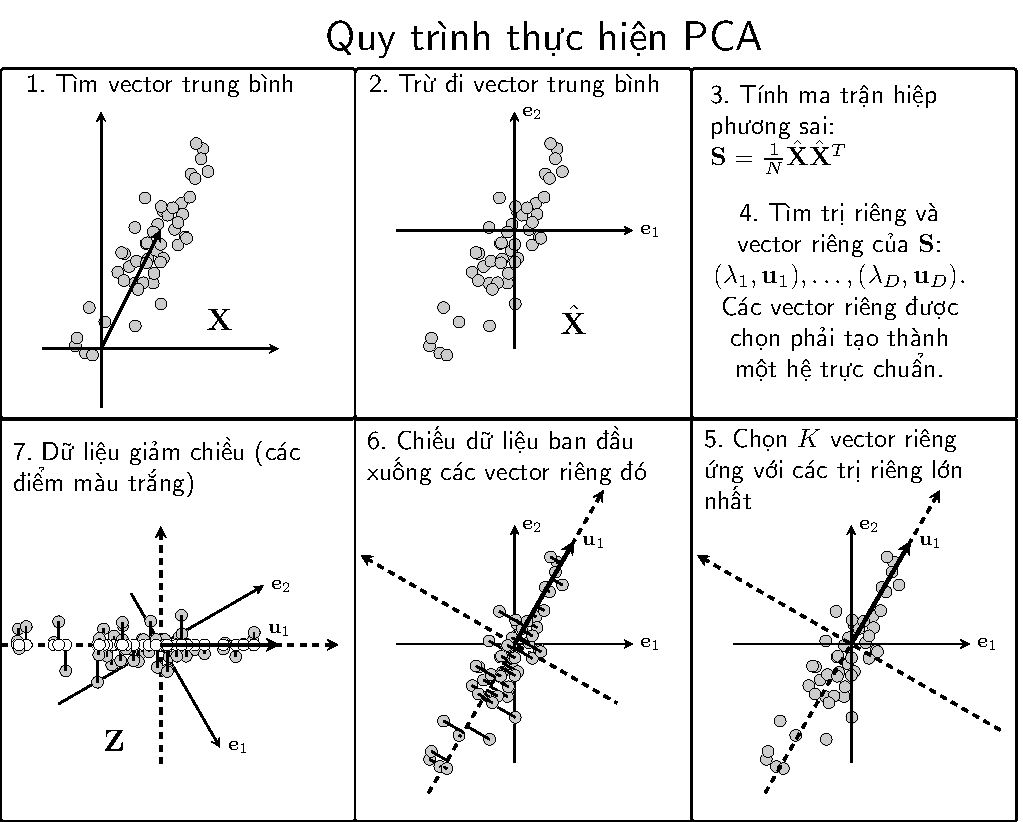
\includegraphics[width = \textwidth]{Chapters/content/27_pca/latex/pca_procedure.pdf}
    \caption[]{Các bước thực hiện PCA.}
    \label{fig:27_5}
\end{figure}
% ******************************************************************************

\section{Liên hệ với phân tích giá trị suy biến}
PCA và SVD có mối quan hệ đặc biệt với nhau. Xin phép nhắc lại hai điểm đã trình bày dưới đây:


\subsection{SVD cho bài toán xấp xỉ hạng thấp tốt nhất}
Nghiệm của bài toán xấp xỉ một ma trận bởi một ma trận có hạng không vượt quá $k$:
\begin{equation}
    \label{eqn:28_1}
    \begin{aligned}
        \min_{\mathbf{A}} & \|\bX - \mathbf{A}\|_F      \\\
        \text{thoả mãn:}~ & \text{rank}(\mathbf{A}) = K
    \end{aligned}
\end{equation}
chính là SVD cắt ngọn của $\mathbf{A}$.

Cụ thể, nếu SVD của $\bX
    \in\mathbb{R}^{D\times N}$ là
\begin{equation}
    \bX = \bU\mathbf{\Sigma}\mathbf{V}^T
\end{equation}
với $\bU \in \mathbb{R}^{D \times D}$ và $\mathbf{V}\in \mathbb{R}^{N\times N}$
là các ma trận trực giao và $\mathbf{\Sigma} \in \mathbb{R}^{D \times N}$ là ma
trận đường chéo (không nhất thiết vuông) với các phần tử trên đường chéo không
âm giảm dần. Nghiệm của bài toán \eqref{eqn:28_1} chính là:
\begin{equation}
    \label{eqn:28_2}
    \mathbf{A} = \bU_K \mathbf{\Sigma}_K \mathbf{V}_K^T
\end{equation}
với $\bU \in \mathbb{R}^{D \times K}$ và $\mathbf{V}\in \mathbb{R}^{N\times K}$
là các ma trận tạo bởi $K$ cột đầu tiên của $\bU$ và $\mathbf{V}$,
$\mathbf{\Sigma}_K \in \mathbb{R}^{K \times K}$ là ma trận đường chéo con ứng
với $K$ hàng đầu tiên và $K$ cột đầu tiên của $\mathbf{\Sigma}$.


\subsection{Ý tưởng của PCA}
Như đã chứng minh ở \eqref{eqn:27_10}, PCA là bài toán đi tìm ma trận
trực giao $\bU$ và ma trận mô tả dữ liệu ở không gian thấp chiều $\mathbf{Z}$
sao cho việc xấp xỉ sau đây là tốt nhất:
\begin{equation}
    \label{eqn:28_3}
    \bX \approx \tilde{\bX} = \bU_K \mathbf{Z} + \what{\bU}_K \what{\bU}_K^T\bar{\mathbf{x}}\mathbf{1}^T
\end{equation}
với $\bU_K, \what{\bU}_K$ lần lượt là các ma trận được tạo bởi $K$ cột đầu tiên
và $D-K$ cột cuối cùng của ma trận trực giao $\bU$, và $\bar{\mathbf{x}}$ là
vector trung bình của dữ liệu.

{Giả sử rằng vector trung bình $\bar{\mathbf{x}} = \mathbf{0}$}. Khi đó, \eqref{eqn:28_3} tương đương với
\begin{equation}
    \label{eqn:28_4}
    \bX \approx \tilde{\bX} = \bU_K \mathbf{Z}
\end{equation}
Bài toán tối ưu của PCA sẽ trở thành:
\begin{equation}
    \label{eqn:28_5}
    \begin{aligned}
        \bU_K, \mathbf{Z} & = & \arg \min_{\bU_K, \mathbf{Z} } \|\bX - \bU_K
        \mathbf{Z}\|_F                                                         \\\
        \text{thoả mãn:}  &   & \bU_K^T \bU_K = \mathbf{I}_K                 &
    \end{aligned}
\end{equation}
với $\mathbf{I}_K \in \mathbb{R}^{K\times K}$ là ma trận đơn vị trong không gian $K$ chiều và điều kiện ràng buộc để đảm bảo các cột của $\bU_K$ tạo thành một hệ trực chuẩn.


\subsection{Quan hệ giữa hai phương pháp}
Có thể nhận ra nghiệm của bài toán \eqref{eqn:28_5} chính là
\begin{align*}
    \bU_K \quad \text{trong}\quad~\eqref{eqn:28_5}     & = \bU_K \quad\text{trong} \quad
    \eqref{eqn:28_2}                                                                                                                 \\\
    \mathbf{Z} \quad\text{trong}\quad~\eqref{eqn:28_5} & = \mathbf{\Sigma}_K \mathbf{V}_K^T \quad\text{trong} \quad \eqref{eqn:28_2}
\end{align*}
Như vậy, nếu các điểm dữ liệu được biểu diễn bởi các cột của một ma trận, và
trung bình các cột của ma trận đó là vector không thì nghiệm của bài toán PCA được rút ra trực tiếp từ SVD cắt ngọn của
ma trận đó. Nói cách khác, việc đi tìm nghiệm cho PCA chính là việc giải một
bài toán phân tích ma trận thông qua SVD.


\section{Làm thế nào để chọn số chiều của dữ liệu mới}

Một câu hỏi được đặt ra là, làm thế nào để chọn giá trị $K$  --  chiều của dữ
liệu mới  --  với từng dữ liệu cụ thể?

Thông thường, $K$ được chọn dựa trên việc {lượng thông tin muốn giữ lại}. Ở đây, toàn bộ thông tin chính là tổng phương sai của toàn bộ các chiều dữ liệu. Lượng dữ liệu muốn dữ lại là tổng phương sai của dữ liệu trong hệ trục toạ độ mới.

Nhắc lại rằng trong mọi hệ trục toạ độ, tổng phương sai của dữ liệu là như nhau
và bằng tổng các trị riêng của ma trận hiệp phương sai $\sum_{i=1}^D
    \lambda_i$. Thêm nữa, PCA giúp giữ lại lượng thông tin (tổng các phương sai) là
$\sum_{i=1}^K \lambda_i$. Vậy ta có thể coi biểu thức:
\begin{equation}
    \label{eqn:28_6}
    r_K = \frac{\sum_{i=1}^K \lambda_i}{\sum_{j=1}^D \lambda_j}
\end{equation}
là tỉ lệ thông tin được giữ lại khi số chiều dữ liệu mới sau PCA là $K$. Như
vậy, giả sử ta muốn giữ lại 99\% dữ liệu, ta chỉ cần chọn $K$ là số tự nhiên
nhỏ nhất sao cho $r_K \geq 0.99$.

Khi dữ liệu phân bố quanh một không gian con, các giá trị phương sai lớn nhất
ứng với các $\lambda_i$ đầu tiên cao gấp nhiều lần các phương sai còn lại.
Khi đó, ta có thể chọn được $K$ khá nhỏ để đạt được $r_K \geq 0.99$.


\section{Lưu ý về tính toán phân tích thành phần chính}
Có hai trường hợp trong thực tế mà chúng ta cần lưu ý về PCA. Trường hợp thứ
nhất là lượng dữ liệu có được nhỏ hơn rất nhiều so với số chiều dữ liệu. Trường
hợp thứ hai là khi lượng dữ liệu trong tập huấn luyện rất lớn, việc tính toán ma trận hiệp phương sai và trị riêng đôi khi trở nên
bất khả thi. Có những hướng giải quyết hiệu quả cho các trường hợp này.

{Trong mục này, ta sẽ coi như dữ liệu đã được chuẩn hoá, tức đã được trừ đi
vector kỳ vọng. Khi đó, ma trận hiệp phương sai sẽ là $\mathbf{S} =
    \frac{1}{N}\bX\bX^T$.}

\subsection{Số chiều dữ liệu nhiều hơn số điểm dữ liệu}

Đó là trường hợp $D > N$, tức ma trận dữ liệu $\bX$ là một \textit{ma trận cao}.
Khi đó, số trị riêng khác không của ma trận hiệp phương sai $\mathbf{S}$ sẽ
không vượt quá hạng của nó, tức không vượt quá $N$. Vậy ta cần chọn $K \leq N$
vì không thể chọn ra được nhiều hơn $N$ trị riêng khác không của một ma trận có hạng
bằng $N$.

Việc tính toán các trị riêng và vector riêng cũng có thể được thực hiện một cách hiệu quả dựa trên các tính chất sau đây:
\begin{enumerate}
    \item  Trị riêng của $\mathbf{A}$ cũng là trị riêng của $k\mathbf{A}$ với $k \neq 0$ bất kỳ. Điều này có thể được suy ra trực tiếp từ định nghĩa của trị riêng và vector riêng.


    \item Trị riêng của $\mathbf{AB}$ cũng là trị riêng của
          $\mathbf{BA}$ với $\mathbf{A} \in \mathbb{R}^{d_1 \times d_2}, \mathbf{B} \in \mathbb{R} ^{d_2 \times d_1}$ là các ma trận bất kỳ và $d_1, d_2$ là các số tự nhiên khác không bất kỳ.

          Như vậy, thay vì tìm trị riêng của ma trận hiệp phương sai $\mathbf{S} \in \mathbb{R}^{D\times D}$, ta đi tìm trị riêng của ma trận $\mathbf{T} = \bX^T \bX \in \mathbb{R}^{N \times N}$ có số chiều nhỏ hơn (vì $N < D$).

    \item Nếu $(\lambda, \mathbf{u})$ là một cặp trị riêng,
          vector riêng của $\mathbf{T}$ thì $(\lambda, \mathbf{Xu})$ là một cặp trị
          riêng, vector riêng của $\mathbf{S}$. Thật vậy:
          \begin{eqnarray}
              \label{eqn:28_8}
              \bX^T \mathbf{Xu} = \bT\bu = \lambda \mathbf{u}
              \Rightarrow (\bX\bX^T)(\mathbf{Xu}) = \lambda (\mathbf{Xu} )
          \end{eqnarray}
          Dấu bằng thứ nhất xảy ra theo định nghĩa của trị riêng và vector riêng.
\end{enumerate}

Như vậy, ta có thể hoàn toàn tính được trị riêng và vector riêng của ma trận
hiệp phương sai $\bS$ dựa trên một ma trận $\bT$ có kích thước nhỏ hơn. Việc
này trong nhiều trường hợp khiến thời gian tính toán giảm đi đáng kể.

% \subsubsection{Chuẩn hoá các vector riêng}

% \textit{Nhắc lại định nghĩa không gian riêng: Không gian riêng ứng với trị riêng của một ma trận là không gian sinh (span subspace) tạo bởi toàn bộ các vector riêng ứng với trị riêng đó.}

% Việc cuối cùng phải làm là chuẩn hoá các vector riêng tìm được sao cho chúng tạo thành một hệ trực chuẩn. Việc này có thể dựa trên hai điểm sau đây:

% \textbf{Thứ nhất}, nếu $\mathbf{A}$ là một ma trận đối xứng, $(\lambda_1,
% \mathbf{x}_1), (\lambda_2, \mathbf{x}_2)$ là các cặp (trị riêng, vector riêng)
% của $\mathbf{A}$ với $\lambda_1 \neq \lambda_2$, thì
% $\mathbf{x}_1^T\mathbf{x}_2 = 0$. Nói cách khác, hai vector bất kỳ trong hai
% không gian riêng khác nhau của một ma trận đối xứng trực giao với nhau.
% Chứng mình:
% \begin{eqnarray}
%   \mathbf{x}_2^T \mathbf{Ax}_1 = \mathbf{x}_1^T \mathbf{Ax}_2 = \lambda_1 \mathbf{x}_2^T \mathbf{x}_1 = \lambda_2 \mathbf{x}_1^T \mathbf{x}_2 \Rightarrow \mathbf{x}_1^T \mathbf{x}_2 = 0
% \end{eqnarray}
% Dấu bằng cuối cùng xảy ra vì $\lambda_1 \neq \lambda_2$.

% \textbf{Thứ hai}, với các trị riêng độc lập tìm được trong một không gian riêng,
% ta có thể dùng quá trình trực giao hoá Gram-Schmit để chuẩn hoá chúng về một hệ
% trực
% chuẩn.

% Kết hợp hai điểm trên, ta có thể thu được các vector riêng tạo thành một hệ trực chuẩn, chính là ma trận $\bU_K$ trong PCA.


\subsection{Với các bài toán quy mô lớn}
Trong rất nhiều bài toán quy mô lớn, ma trận hiệp phương sai là một ma trận rất lớn. Ví dụ, có một triệu bức ảnh
1000 $\times$ 1000 pixel, như vậy $D = N = 10^6$ là các số rất lớn, việc trực
tiếp tính toán trị riêng và vector riêng cho ma trận hiệp phương sai là không
khả thi. Lúc này, các trị riêng và vector riêng của ma trận hiệp phương sai thường được tính thông qua \textit{power method}
(\url{https://goo.gl/eBRPxH}).

\section{Ứng dụng trong nén dữ liệu đa phương tiện dạng ảnh}

\subsection{Triển khai thuật toán PCA bằng ngôn ngữ python}

Để thực hiện triển khai thuật toán chúng ta sẽ thực hiện bằng 6 bước sau :

\begin{itemize}
    \item Tính hiệu giá trị của giá trị mỗi cột và giá trị trung bình của cột đó
    \item Tính ma trận hiệp phương sai dữ liệu
    \item Tính toán giá trị riêng và vector riêng của ma trận hiệp phương sai
    \item Sắp xêp các giá trị riêng theo chiều tăng dần
    \item Chọn tập con trong tập giá trị riêng đã sắp xếp
    \item Chuyển đổi dữ liệu
\end{itemize}

\newpage
Đây là đoạn code thực hiện các bước trên sử dụng ngôn ngữ python và thư viện numpy (1 thư viện hỗ trợ tính toán)
\begin{lstlisting}[language=Python]
    import numpy as np
 
    def PCA(X , num_components):
        
        #Step-1
        X_meaned = X - np.mean(X , axis = 0)
        
        #Step-2
        cov_mat = np.cov(X_meaned , rowvar = False)
        
        #Step-3
        eigen_values , eigen_vectors = np.linalg.eigh(cov_mat)
        
        #Step-4
        sorted_index = np.argsort(eigen_values)[::-1]
        sorted_eigenvalue = eigen_values[sorted_index]
        sorted_eigenvectors = eigen_vectors[:,sorted_index]
        
        #Step-5
        eigenvector_subset = sorted_eigenvectors[:,0:num_components]
        
        #Step-6
        X_reduced = np.dot(eigenvector_subset.transpose() , X_meaned.transpose() ).transpose()
        
        return X_reduced
    
\end{lstlisting}

\
\newpage
\subsection{Chương trình nén sử dụng PCA bằng ngôn ngữ python}
\subsubsection{Mô hình tổng quan của chương trình}

Mô hình tập trung vào chứng minh tính giảm chiều dữ liệu của thuật toán PCA

\begin{center}
    \begin{figure}[htp]
        \begin{center}
            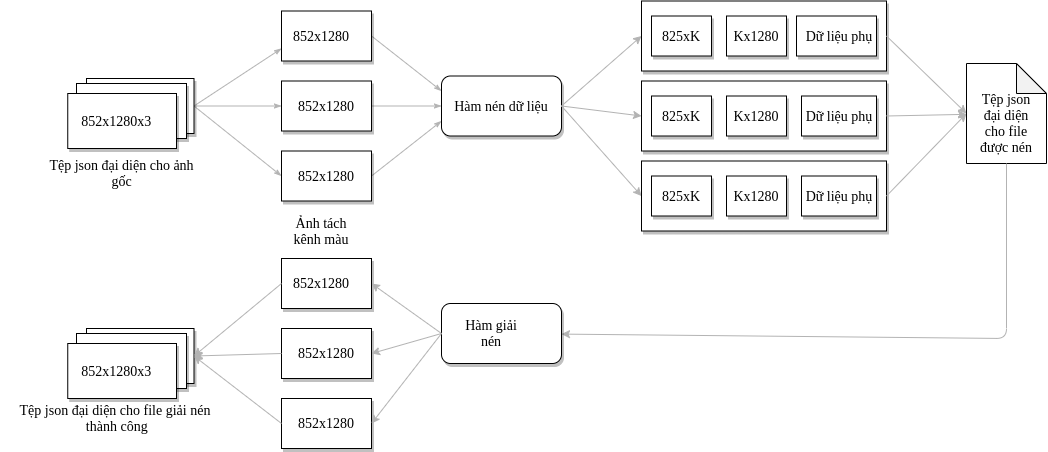
\includegraphics[width=\textwidth,height=\textheight,keepaspectratio]{Chapters/content/27_pca/model.png}
        \end{center}
        \caption{Mô tả chương trình}
        \label{fig:27_6}
    \end{figure}
\end{center}

\subsubsection{Nén và lưu trữ dữ liệu nén}

Hàm sử dụng để nén các ma trận ảnh riêng biệt kích thước mxn:


Hàm này đươc thực thi với các tham số  là ma trận các điểm ảnh và phần trăm nén ảnh.
\newpage
\begin{lstlisting}[language=Python]
    def compress_img(img, percen):
        '''compress image with percent'''

        pca = PCA().fit(img)
        var_cumu = np.cumsum(pca.explained_variance_ratio_)*100
        k = np.argmax(var_cumu > percen)

        ipca = IncrementalPCA(n_components=k)
        img_compressed = ipca.fit_transform(img)
        list_att = ['components_', 'mean_', 'explained_variance_', 'whiten']
        ipca_att = {}
        for att in list_att:
            ipca_att[att] = ipca.__getattribute__(att)
        return k, img_compressed, ipca_att
    
\end{lstlisting}

Kết quả các giá trị mà hàm này trả về :
\begin{itemize}
    \item Số lượng thành phần chính cần thiết để có phần trăm nén tương ứng
    \item Ma trận rút gọn theo các thành phần ở trên
    \item Các tham số cần thiết cho việc phục hồi lại ma trận ban đầu (đương nhiều là ma trận phục hội sẽ bị mất mát dữ liệu)
\end{itemize}

\begin{center}
    \begin{figure}[htp]
        \begin{center}
            
\includegraphics[width=\textwidth,height=\textheight,keepaspectratio]{Chapters/content/27_pca/imgg_origin.jpg}
        \end{center}
        \caption{Ảnh đưa vào bộ nén}
        \label{fig:27_7}
    \end{figure}
\end{center}

\subsubsection{Giải nén từ dữ liệu nén}

Hàm giải nén được thực thi với các tham số truyền vào là các giá trị kết quả của hàm nén

Hàm này chịu trách nghiệm phục hồi lại ảnh với kích thước ban đầu

\begin{lstlisting}[language=Python]
    def extract_img(result_compressed):
        k = result_compressed[0]
        ipca = IncrementalPCA(n_components=k)
        img_compressed = result_compressed[1]
        dict_att = result_compressed[2]
        for key in dict_att.keys():
            ipca.__setattr__(key, dict_att[key])
        # print((dict_att['mean_']))
        img_extracted = ipca.inverse_transform(img_compressed)
        return img_extracted
    
\end{lstlisting}

\subsubsection{Phục hồi ảnh từ các ma trận được giải nén}

Đoạn mã sau thể hiện sự gộp các ma trận của 3 kênh màu RGB từ ảnh ban đầu sau 1 chuỗi xử lý nén và giải nén

\begin{lstlisting}[language=Python]
    # read json file
    img_compressed1 = {}
    with open(path+'imgj_compressed.json', 'r') as f:
        img_compressed1 = json.load(f)

    # extract image
    img_extracted = [extract_img(img_tmp)for img_tmp in img_compressed1]
    img_extracted = concat_img(*img_extracted)
    
\end{lstlisting}

Biến \pythoninline{img_extracted} lưu ảnh hoàn thiện sau khi đã gộp lại từ các ma trận của 3 kênh màu RGB

\begin{center}
    \begin{figure}[htp]
        \begin{center}
            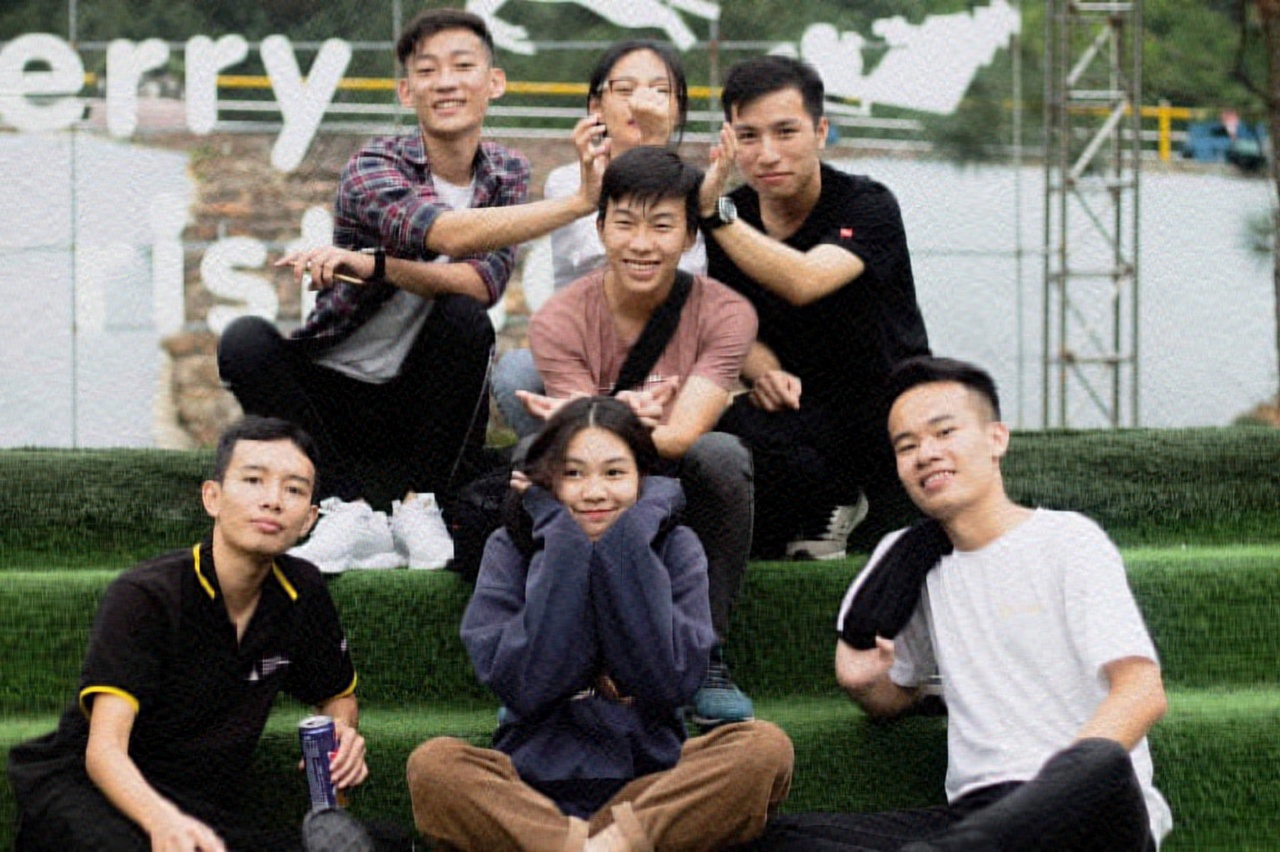
\includegraphics[width=\textwidth,height=\textheight,keepaspectratio]{Chapters/content/27_pca/imgg_extracted.jpg}
        \end{center}
        \caption{Ảnh giải nén sau khi đã được gộp từ các ma trận của 3 kênh màu}
        \label{fig:27_8}
    \end{figure}
\end{center}



\newpage
\subsubsection{Biểu diễn hiệu quả nén}

\begin{center}
    \begin{figure}[htp]
        \begin{center}
            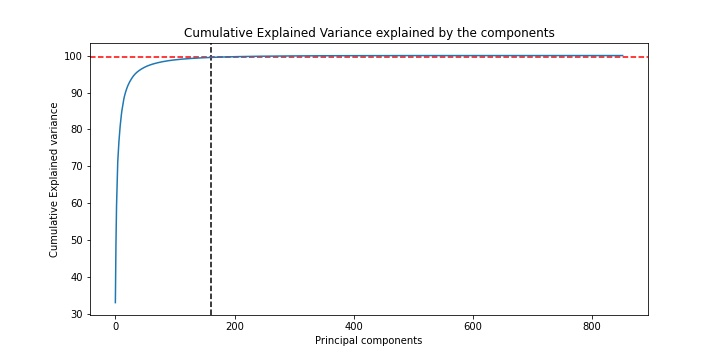
\includegraphics[scale=.5]{Chapters/content/27_pca/cumsum.jpg}
        \end{center}
        \caption{Đường thể hiện tổng cộng dồn của các giá trị riêng thành phần chính}
        \label{fig:27_9}
    \end{figure}
\end{center}

Biểu đồ trên cho thấy khi ta lựa chọn số phần trăm nén là 99$\%$ thì số lượng thành phần được chọn cũng chỉ bằng $1/4$ tổng số thành phần.


Nên khi gặp những ảnh có đường biểu diễn như thế thì hiệu quả nén được sẽ lớn nhưng mất mát thì nhỏ.

\begin{center}
    \begin{figure}[htp]
        \begin{center}
            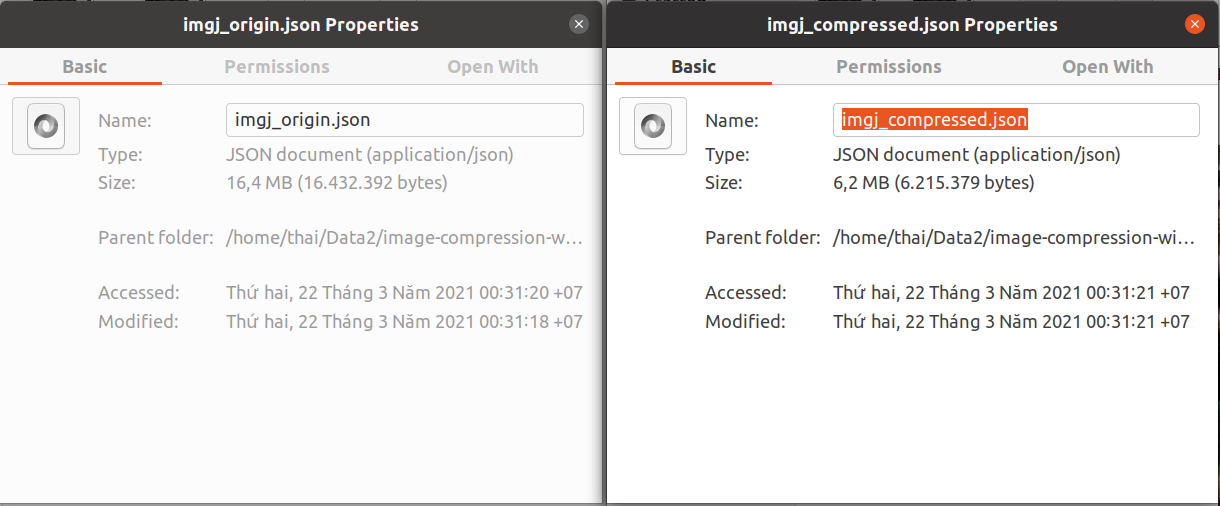
\includegraphics[width=\textwidth,height=\textheight,keepaspectratio]{Chapters/content/27_pca/compare.png}
        \end{center}
        \caption{So sánh tệp trước và sau khi nén}
        \label{fig:27_10}
    \end{figure}
\end{center}

Kết quả chúng ta đã thu được tệp nén có kích thước 6.4 MB so với 16.4 MB của tệp gốc, tức là chỉ bằng $40\%$ so với tệp gốc.
\newpage
\subsubsection{So sánh hiệu quả nén với các định dạng ảnh khác nhau}
\begin{center}
    \begin{figure}[htp]
        \begin{center}
            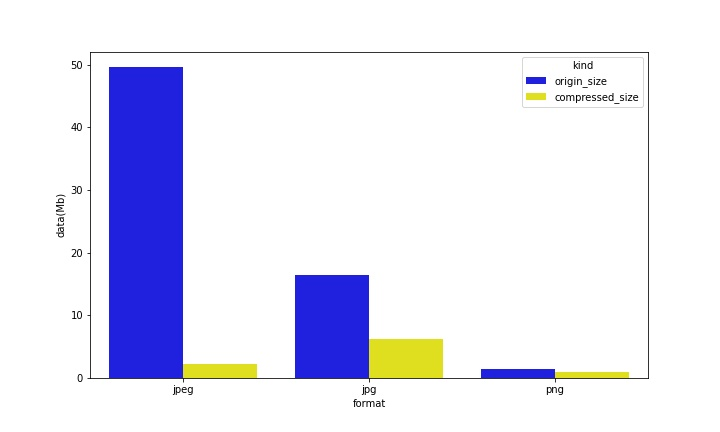
\includegraphics[width=\textwidth,height=\textheight,keepaspectratio]{Chapters/content/27_pca/barplot.jpg}
        \end{center}
        \caption{Đối chiếu kích thước tệp nén và tệp gốc của các định dạng ảnh khác nhau}
        \label{fig:27_11}
    \end{figure}
\end{center}

Chú thích :
\begin{itemize}
    \item Cột màu xanh : dung lượng của file gốc
    \item Cột màu vàng : dung lượng của file nén
\end{itemize}

Kết luận :
\begin{itemize}
    \item Đối với ảnh định dạng jpeg thì hiệu quả nén cao hơn so với các định dạng khác
    \item Đối với ảnh định dạng png thì hiệu quả nén rất thấp do ảnh png là ảnh được tạo thành từ các vector chứ không phải từ những điểm ảnh cố định
\end{itemize}


% \begin{document}
% \centering
% 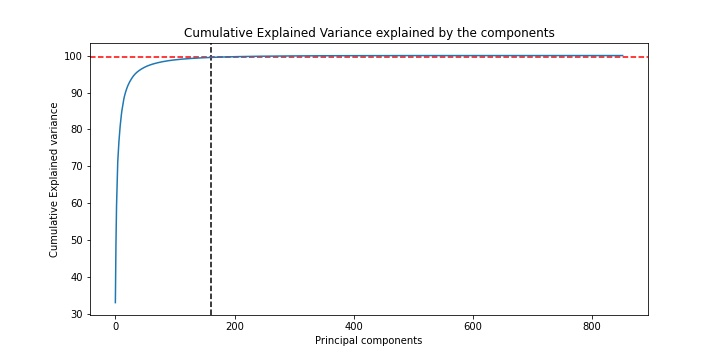
\includegraphics[width = \textwidth]{Chapters/content/27_pca/cumsum.jpg}
% \caption{Ví dụ về ảnh của một người trong Yale Face Database.}
% \end{document}



\section{Một số ứng dụng khác}
Ứng dụng đầu tiên của PCA chính là việc giảm chiều dữ liệu, giúp
việc lưu trữ và tính toán được thuận tiện hơn. Thực tế cho thấy, nhiều khi làm
việc trên dữ liệu đã được giảm chiều mang lại kết quả tốt hơn so với dữ liệu
gốc. Thứ nhất, có thể phần dữ liệu mang thông tin nhỏ bị lược đi chính là phần
gây nhiễu, những thông tin quan trọng hơn đã được giữ lại. Thứ hai, số điểm dữ
liệu nhiều khi ít hơn số chiều dữ liệu. Khi có quá ít dữ liệu và số chiều dữ
liệu quá lớn, quá khớp rất dễ xảy ra. Việc giảm chiều dữ liệu phần nào giúp
khắc phục hiện tượng này.

Dưới đây là hai ví dụ về ứng dụng của PCA trong bài toán phân loại khuôn mặt và dò điểm bất thường.

\subsection{Khuôn mặt riêng}
\index{khuôn mặt riêng -- eigenface}
\index{eigenface -- khuôn mặt riêng}
\textit{Khuôn mặt riêng} (eigenface) từng là một trong những kỹ thuật phổ biến
trong bài toán nhận dạng khuôn mặt. Ý tưởng của khuôn mặt riêng là đi tìm một
không gian có số chiều nhỏ hơn để mô tả mỗi khuôn mặt, từ đó sử dụng vector
trong không gian thấp chiều này như vector đặc trưng cho bộ phân loại. Điều đáng
nói là một bức ảnh khuôn mặt có kích thước khoảng 200 $\times$ 200 sẽ có số
chiều là 40k -- một số rất lớn, trong khi đó, vector đặc trưng thường chỉ có số
chiều bằng vài trăm hoặc vài nghìn. Khuôn mặt riêng thực ra chính là PCA. Các
khuôn mặt riêng chính là các vector riêng ứng với những trị riêng lớn nhất của
ma trận hiệp phương sai.

\index{cơ sở dữ liệu khuôn mặt Yale -- Yale face database}
\index{Yale face database -- cơ sở dữ liệu khuôn mặt Yale}
Trong phần này, chúng ta làm một thí nghiệm nhỏ trên \textit{cơ sở dữ liệu
    khuôn mặt Yale} (\url{https://goo.gl/LNg8LS}). Các bức ảnh trong thí nghiệm
này đã được căn chỉnh cho cùng với kích thước và khuôn mặt nằm trọn vẹn trong
một hình chữ nhật có kích thước $116 \times  98$ điểm ảnh. Có tất cả 15 người khác
nhau, mỗi người có 11 bức ảnh được chụp ở các điều kiện ánh sáng và cảm xúc khác
nhau, bao gồm \pythoninline{'centerlight', 'glasses', 'happy', 'leftlight',
    'noglasses', 'normal', 'rightlight','sad', 'sleepy', 'surprised'}, và
\pythoninline{'wink'}. Hình \ref{fig:28_1} minh hoạ các bức ảnh của
người có id là 10.
% <hr>
% <div class="imgcap">
% <img src ="/assets/28_pca2/yaleb_exs.png" align = "center" width = "800">
% </div>
% <div class = "thecap" align = "left">Hình 1: Ví dụ về ảnh của một người trong Yale Face Database. </div>
% <hr>

\begin{figure}[t]
    \centering
    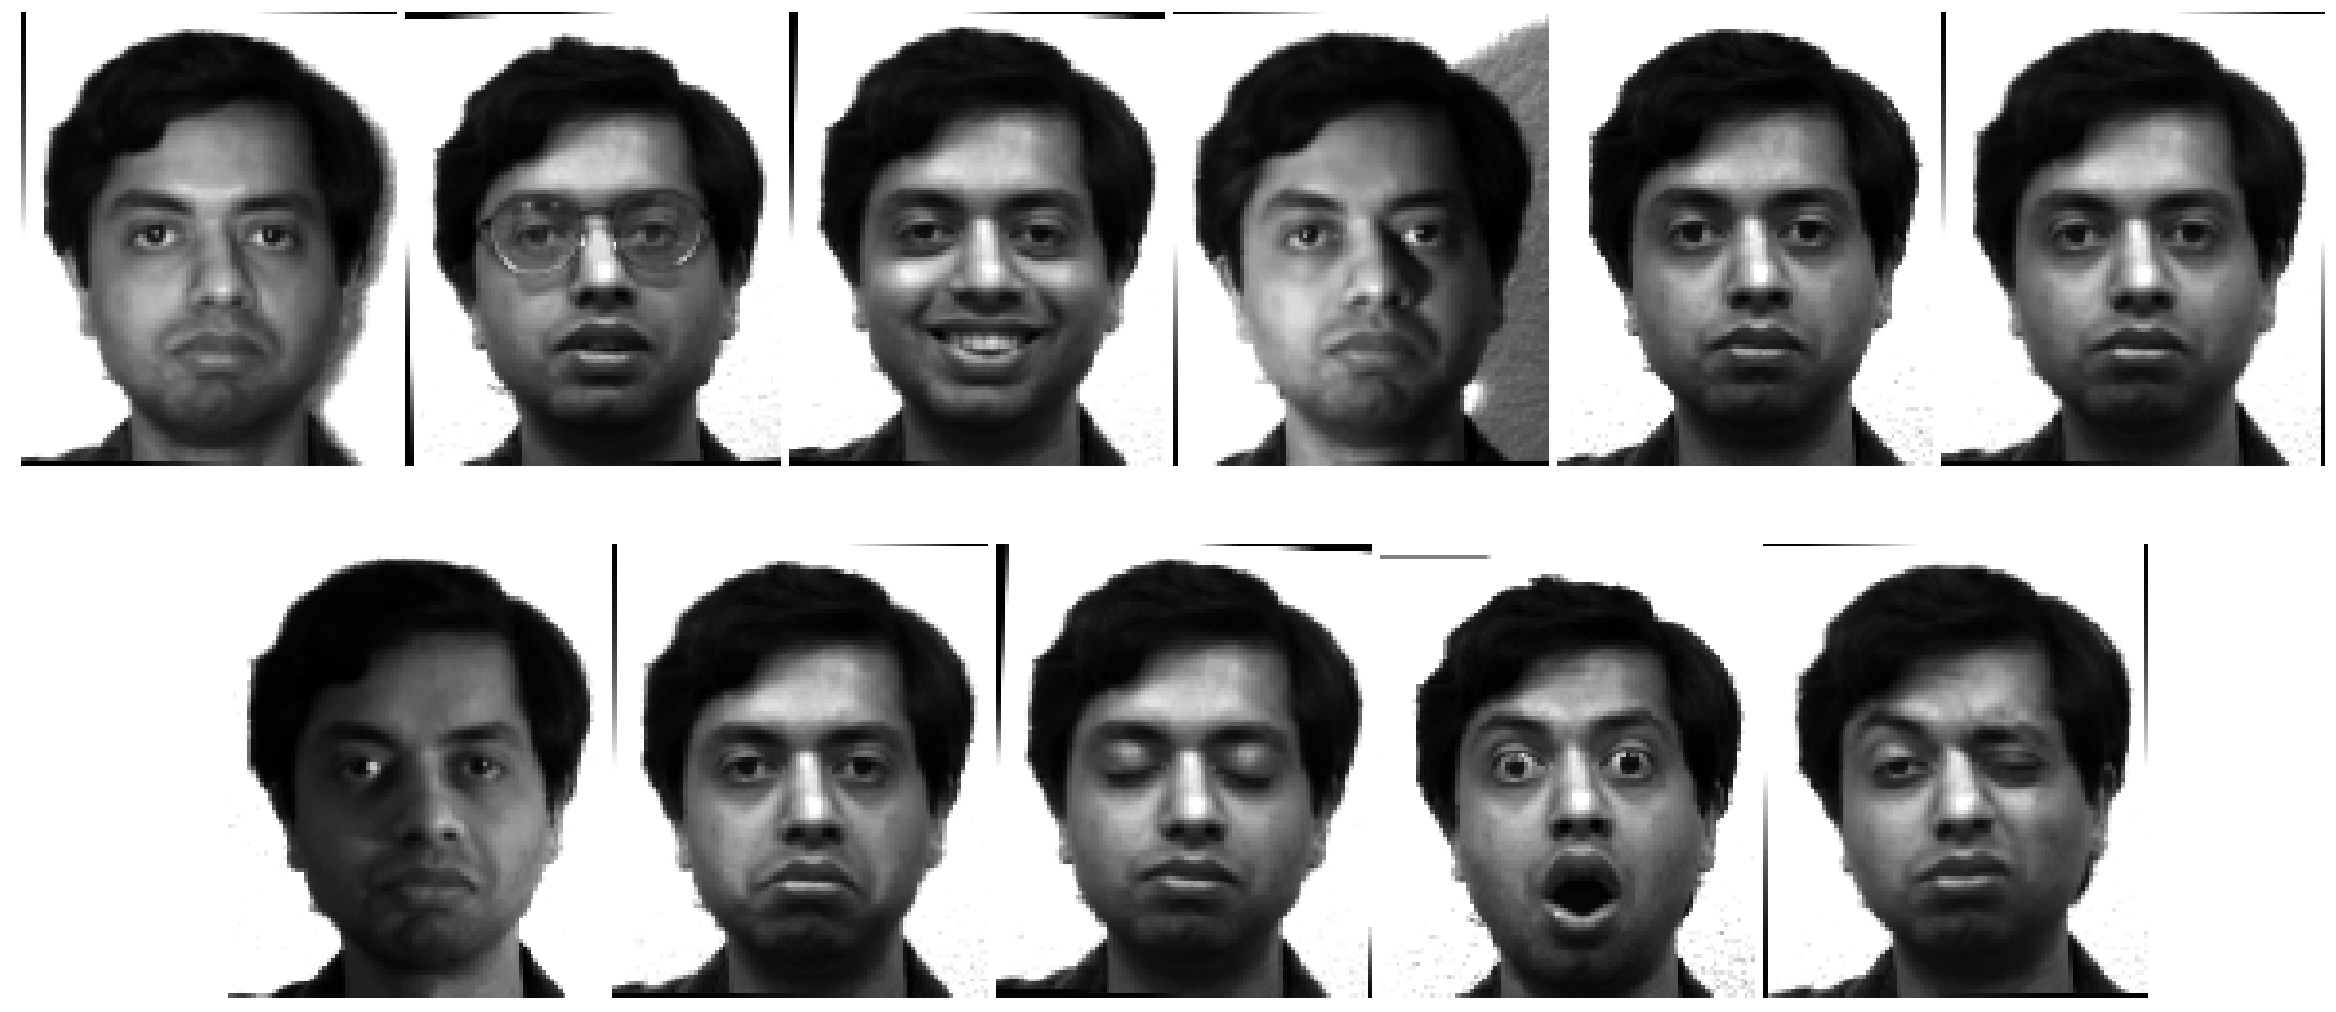
\includegraphics[width = \textwidth]{Chapters/content/28_pca2/latex/yaleb_exs.pdf}
    \caption[]{Ví dụ về ảnh của một người trong Yale Face Database.}
    \label{fig:28_1}
\end{figure}

Ta thấy rằng số chiều dữ liệu $116 \times 98 = 11368$ là một số khá
lớn. Tuy nhiên, vì chỉ có tổng cộng $15 \times 11 = 165$ bức ảnh nên ta có thể
nén các bức ảnh này về dữ liệu mới có chiều nhỏ hơn 165. Trong ví dụ này, chúng
ta chọn $K = 100$.

Dưới đây là đoạn code thực hiện PCA cho toàn bộ dữ liệu. Ở đây, PCA trong \pythoninline{sklearn} được sử dụng:
\newpage
\begin{lstlisting}[language=Python]
    from sklearn.decomposition import PCA
    import numpy as np
    import scipy.misc                  # for loading image
    from matplotlib.pyplot import imread
    np.random.seed(1)
    
    # filename structure
    path = 'YALE/unpadded/'  # path to the database
    ids = range(1, 16)  # 15 persons
    states = ['centerlight', 'glasses', 'happy', 'leftlight',
              'noglasses', 'normal', 'rightlight', 'sad',
              'sleepy', 'surprised', 'wink']
    prefix = 'subject'
    surfix = '.pgm'
    # data dimension
    h, w, K = 116, 98, 100  # hight, weight, new dim
    D = h * w
    N = len(states)*15
    # collect all data
    X = np.zeros((D, N))
    cnt = 0
    for person_id in range(1, 16):
        for state in states:
            fn = path + prefix + str(person_id).zfill(2) + '.' + state + surfix
            print(fn)
            X[:, cnt] = imread(fn).reshape(D)
            # misc.imread
            cnt += 1
    
    # Doing PCA, note that each row is a datapoint
    pca = PCA(n_components=K)  # K = 100
    pca.fit(X.T)
    # projection matrix
    U = pca.components_.T
    
\end{lstlisting}

Trong dòng \pythoninline{pca = PCA(n_components=K)}, nếu
\pythoninline{n_components} là một số thực trong khoảng $(0, 1)$, PCA sẽ thực
hiện việc tìm $K$ dựa trên biểu thức~\eqref{eqn:28_6}.

% ******************************************************************************
\begin{figure}[t]
    \centering
    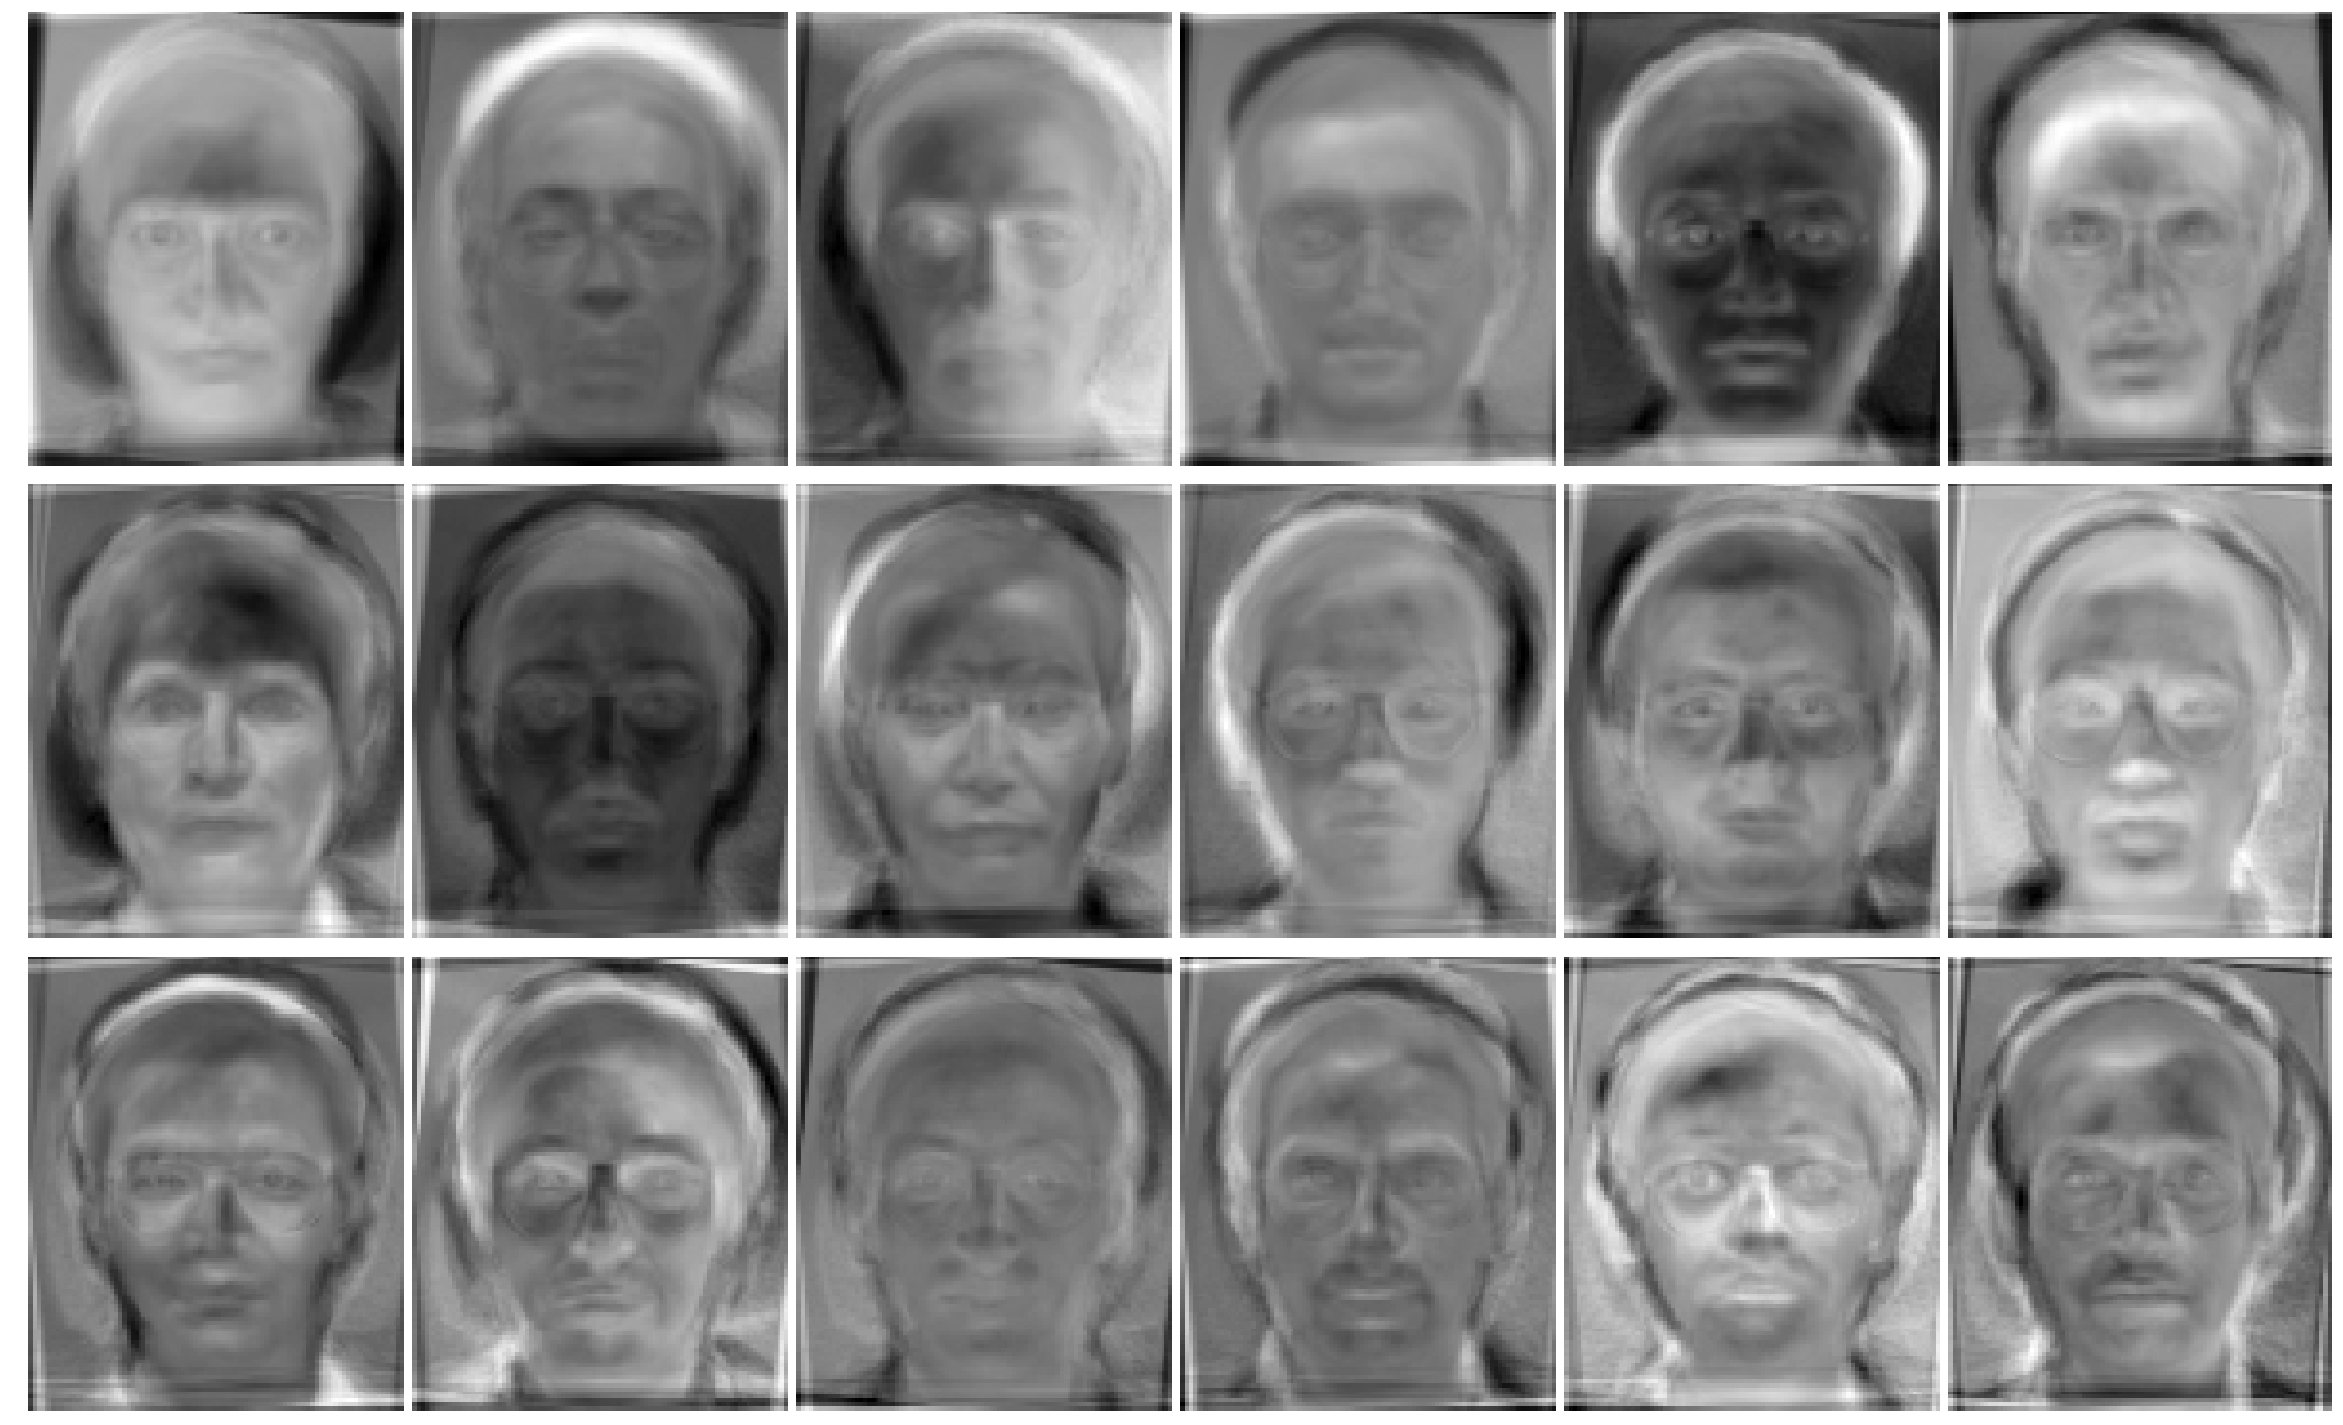
\includegraphics[width = \textwidth]{Chapters/content/28_pca2/latex/yaleb_eig.pdf}
    \caption[]{Các eigenfaces tìm được bằng PCA.}
    \label{fig:28_2}
\end{figure}
% ******************************************************************************

Hình \ref{fig:28_2} biểu diễn 18 vector riêng đầu tiên (18 cột đầu tiên của
$\bU_k$) tìm được bằng PCA. Các vector đã được \pythoninline{reshape} về cùng
kích thước như các bức ảnh gốc. Nhận thấy các
vector thu được ít nhiều mang thông tin của mặt người. Thực tế, một khuôn mặt
gốc sẽ được xấp xỉ như tổng có trọng số của các {khuôn mặt} này. Vì các
vector riêng này đóng vai trò như cơ sở của không gian mới với ít chiều hơn,
chúng còn được gọi là \textit{khuôn mặt riêng} hoặc \textit{khuôn mặt chính}. Từ \textit{chính} được dùng vì nó đi kèm với văn cảnh
của \textit{phân tích thành phần chính}.
% ******************************************************************************
\begin{figure}[t]
    \centering
    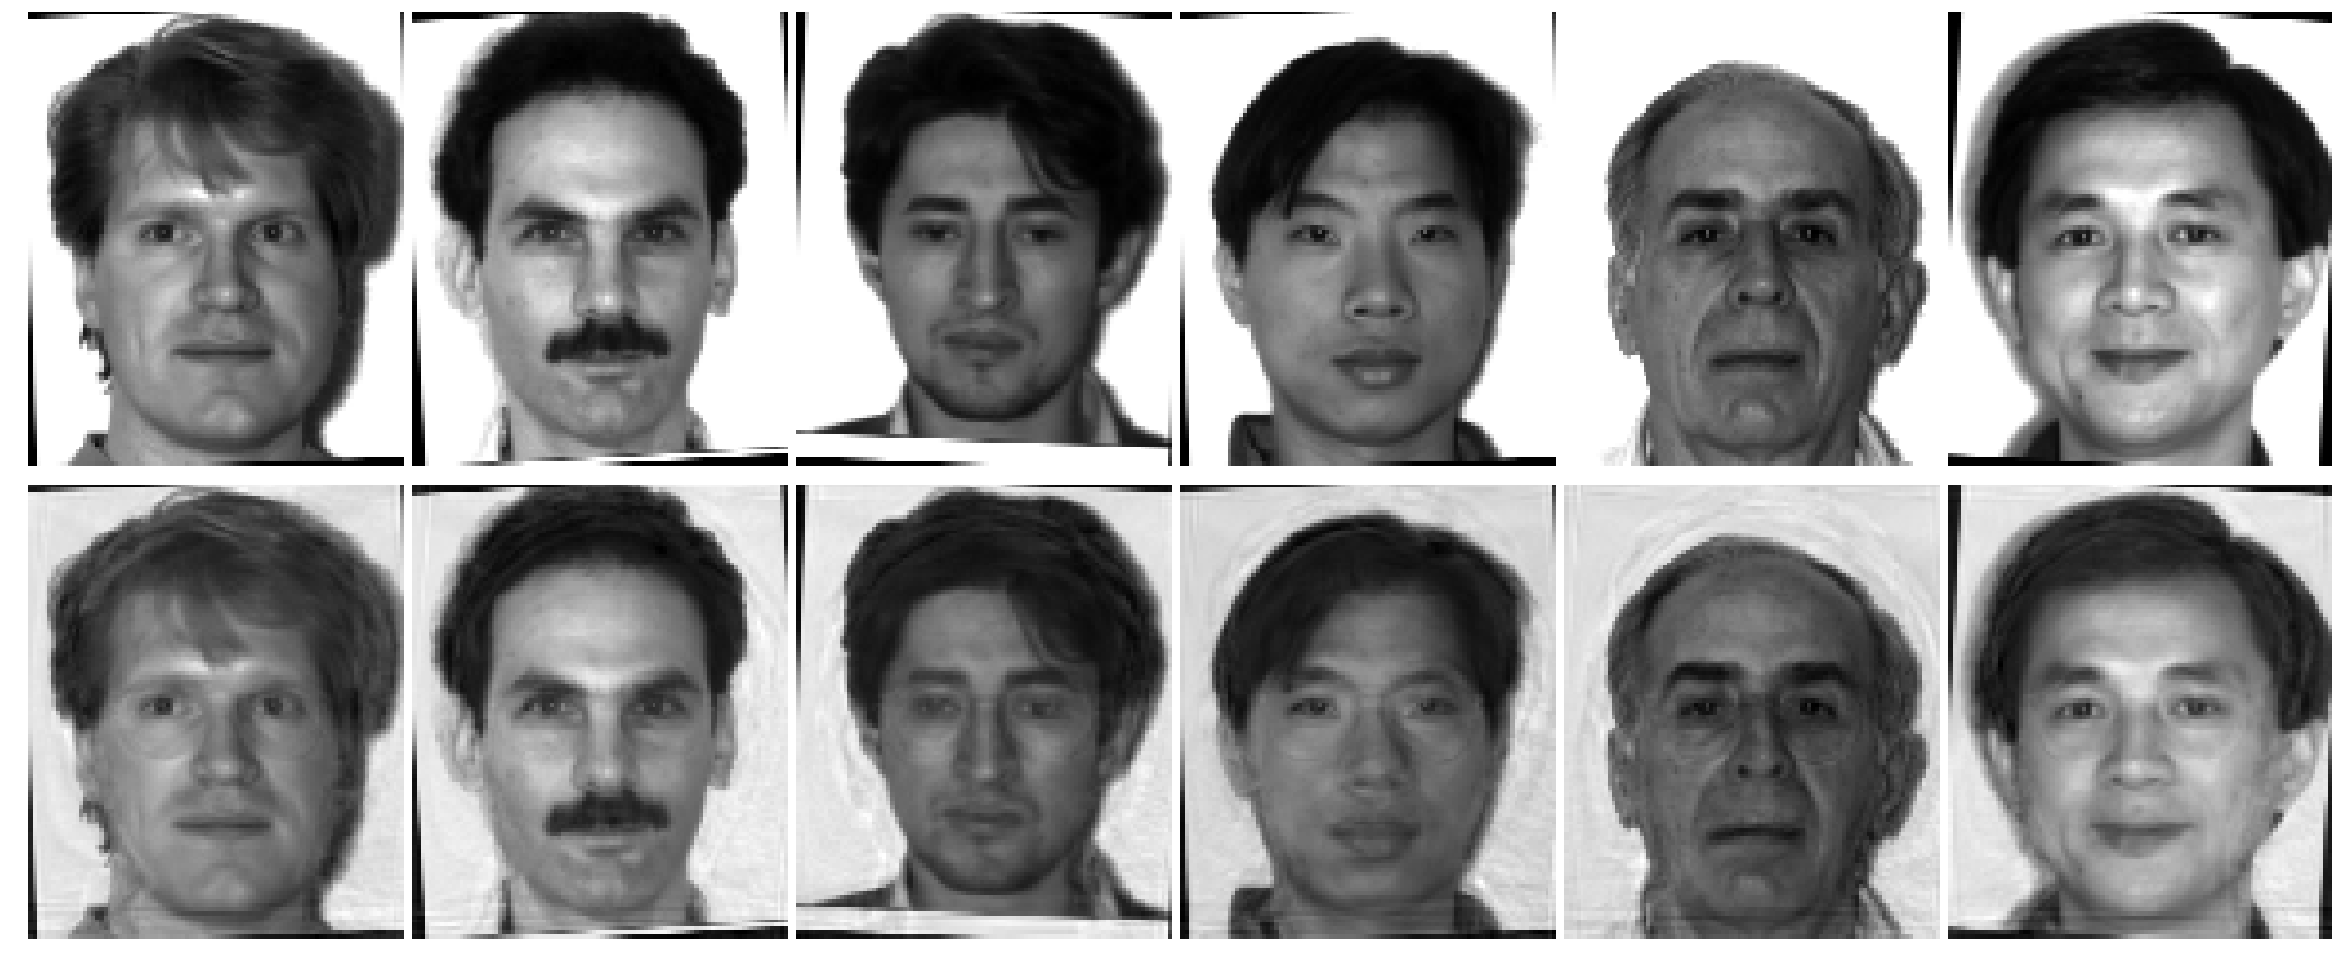
\includegraphics[width = \textwidth]{Chapters/content/28_pca2/latex/yaleb_ori_res.pdf}
    \caption[]{Hàng trên: các ảnh gốc. Hàng dưới: các ảnh được tái tạo dùng khuôn mặt riêng. Ảnh ở hàng dưới có nhiễu nhưng vẫn mang những đặc điểm riêng mà mắt người có thể phân biệt được.}
    \label{fig:28_3}
\end{figure}
% ******************************************************************************

Để xem mức độ hiệu quả của phương pháp này, chúng ta  minh hoạ các bức ảnh gốc và các bức ảnh được xấp xỉ bằng PCA như trên
Hình~\ref{fig:28_3}. Các khuôn mặt nhận được vẫn mang khá đầy đủ thông tin của
các khuôn mặt gốc. Đáng chú ý hơn, các khuôn mặt trong hàng dưới được suy ra
từ một vector 100 chiều, so với 11368 chiều như ở hàng trên.




% Phần còn lại của source code có thể được tìm thấy \href{https://github.com/tiepvupsu/tiepvupsu.github.io/blob/master/assets/28_pca2/python/EigenFaces.ipynb}{tại đây}.

\subsection{Dò tìm điểm bất thường}
Ngoài các ứng dụng về nén và phân loại, PCA còn được sử dụng trong nhiều lĩnh
vực khác. \textit{Dò tìm điểm bất thường} (abnormal detection hoặc {outlier
    detection}) là một trong số đó~\cite{shyu2003novel,lakhina2004diagnosing}.

Ý tưởng cơ bản là giả sử tồn tại một không gian con mà các sự kiện bình thường
nằm gần trong khi các sự kiện bất thường nằm xa không gian con đó. Hơn nữa, số
sự kiện bất thường có một tỉ lệ nhỏ. Như vậy, PCA có thể được sử dụng trên toàn
bộ dữ liệu để tìm ra các thành phần chính, từ đó suy ra không gian con mà các điểm bình thường nằm gần.
Việc xác định một điểm là bình thường hay bất thường được xác định bằng cách đo
khoảng cách từ điểm đó tới không gian con tìm được. Hình~\ref{fig:28_4} minh hoạ
cho việc xác định các sự kiện bất thường bằng PCA.

\begin{figure}[t]
    % caption on side

    \floatbox[{\capbeside\thisfloatsetup{capbesideposition={right,top},capbesidewidth=6.5cm}}]{figure}[\FBwidth]
    {\caption{ PCA cho bài toán dò tìm điểm bất thường. Giả sử
    các sự kiện {bình thường} chiếm đa số và nằm gần  một không
    gian con nào đó. Khi đó, nếu làm PCA trên toàn bộ dữ liệu, không gian con
    thu được gần với không gian con của tập các sự kiện {bình thường}.
    Lúc này, các
    điểm hình tròn to đậm hơn có thể được coi là các sự kiện {bất thường} vì chúng nằm xa không gian con chính.}
    \label{fig:28_4}}
    { % figure here
    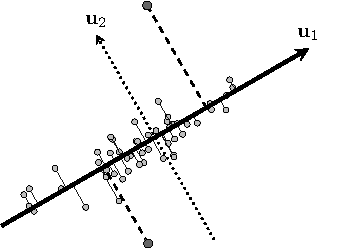
\includegraphics[width=.45\textwidth]{Chapters/content/28_pca2/latex/abnormal.pdf}
    }
\end{figure}


\section{Kết luận}
\begin{itemize}
    \item PCA là phương pháp giảm chiều dữ liệu dựa trên việc tối đa lượng
          thông tin được giữ lại. Lượng thông tin được giữ lại được đo bằng tổng các
          phương sai trên mỗi thành phần của dữ liệu. Lượng dữ liệu sẽ được giữ lại nhiều
          nhất khi các chiều dữ liệu còn lại tương ứng với các vector riêng của trị riêng
          lớn nhất của ma trận hiệp phương sai.

    \item Với các bài toán quy mô lớn, đôi khi việc tính toán trên toàn bộ dữ liệu
          là không khả thi vì vấn đề bộ nhớ. Giải pháp là thực hiện PCA lần đầu
          trên một tập con dữ liệu vừa với bộ nhớ, sau đó lấy một tập con khác để {từ từ} (\textit{incrementally}) cập nhật nghiệm của PCA tới khi hội
          tụ. Ý tưởng này khá giống với mini-batch gradient descent, và được gọi là
          incremental PCA~\cite{zhao2006novel}.


\end{itemize}



\backmatter%%%%%%%%%%%%%%%%%%%%%%%%%%%%%%%%%%%%%%%%%%%%%%%%%%%%%%%
\medskip
\bibliographystyle{abbrv}
\bibliography{refs}

% \printindex
\end{document}
